% !TeX program = xelatex
% Archivo principal: compilar con XeLaTeX + BibTeX.
\documentclass[12pt,letterpaper,oneside]{report}
% DATOS EDITABLES. Título propuesto, ampliado para representar los dos casos.
\newcommand{\TituloMemoria}{Implementación y Evaluación de redes neuronales en un microcontrolador}
\newcommand{\AutorMemoria}{Alonso Castillo Pinto}
\newcommand{\ProfesorGuia}{Alejandro Weinstein}
\newcommand{\ProfesorCorreferente}{Gonzalo Carvajal}
\newcommand{\TituloProfesional}{INGENIERO CIVIL ELECTRÓNICO} % Confirmar denominación oficial.
\newcommand{\CiudadMemoria}{VALPARAÍSO}
\newcommand{\MesMemoria}{MES DEL EXAMEN} % Completar al cerrar la memoria.
\newcommand{\AnioMemoria}{2026}
\newif\ifnotaseditoriales
\notaseditorialesfalse % Cambiar a false para ocultar notas y anexo editorial.
% Modo estricto: falla la compilación si no está Times New Roman.
\newif\iffuenteestricta
\fuenteestrictafalse % Activar en la entrega formal después de instalar la fuente.

\usepackage{fontspec}
% La norma exige Times New Roman. No se distribuye una fuente propietaria.
% Opción 1: cuatro archivos propios en fuentes/ (ver README).
\IfFileExists{fuentes/times.ttf}{
 \setmainfont{times.ttf}[Path=fuentes/,BoldFont=timesbd.ttf,ItalicFont=timesi.ttf,BoldItalicFont=timesbi.ttf]
}{\IfFontExistsTF{Times New Roman}{\setmainfont{Times New Roman}}{
 \iffuenteestricta
  \PackageError{memoria}{Falta Times New Roman}{Suba los cuatro TTF propios a fuentes/.}
 \fi
 \IfFontExistsTF{TeX Gyre Termes}{\setmainfont{TeX Gyre Termes}}{\setmainfont{NimbusRoman-Regular.otf}[BoldFont=NimbusRoman-Bold.otf,ItalicFont=NimbusRoman-Italic.otf,BoldItalicFont=NimbusRoman-BoldItalic.otf]}
 \PackageWarningNoLine{memoria}{Fuente alternativa de previsualizacion. Instale Times New Roman antes de la entrega}
}}
\usepackage[english]{babel}
\babelprovide[main,import]{spanish}
\addto\captionsspanish{\renewcommand{\tablename}{Tabla}\renewcommand{\appendixname}{Anexo}}
\usepackage[left=4cm,right=3cm,top=3cm,bottom=3cm,footskip=1.2cm]{geometry}
\usepackage{setspace}
\onehalfspacing
% 12 pt: espacio natural 14.5 pt; 1.5 interlineado = 18.125 pt.
% Añadir 6.042 pt entre párrafos da 24.167 pt: doble interlineado.
\setlength{\parskip}{6.042pt plus 1pt minus 1pt}
\setlength{\parindent}{1.25cm}
\usepackage{amsmath,amssymb}
\usepackage{graphicx,xcolor,booktabs,array,tabularx,longtable}
\usepackage{caption}
\captionsetup{font=small,labelfont=bf}
\captionsetup[table]{position=top}
\usepackage{float,enumitem,titlesec,fancyhdr,etoolbox}
\usepackage{tikz}
\usetikzlibrary{positioning,arrows.meta}
\usepackage{xurl}
\usepackage[hidelinks,unicode]{hyperref}
\hypersetup{pdftitle={\TituloMemoria},pdfauthor={\AutorMemoria},pdfsubject={Memoria de titulación: evaluación de cuantización en microcontroladores}}
\pagestyle{fancy}\fancyhf{}\fancyfoot[R]{\thepage}
\renewcommand{\headrulewidth}{0pt}
\fancypagestyle{plain}{\fancyhf{}\fancyfoot[R]{\thepage}\renewcommand{\headrulewidth}{0pt}}
\titleformat{\chapter}[block]{\normalfont\bfseries\Large}{\thechapter}{.7em}{}
\titleformat{name=\chapter,numberless}[block]{\normalfont\bfseries\Large\filcenter}{}{0pt}{}
\titlespacing*{\chapter}{0pt}{0pt}{20pt}
\titleformat{\section}{\normalfont\bfseries\large}{\thesection}{.7em}{}
\titleformat{\subsection}{\normalfont\bfseries}{\thesubsection}{.7em}{}
% Un nivel adicional para conservar la jerarquía de los antiguos capítulos.
\setcounter{secnumdepth}{3}\setcounter{tocdepth}{3}
\titleformat{\subsubsection}{\normalfont\bfseries}{\thesubsubsection}{.7em}{}
\addto\captionsspanish{\renewcommand{\contentsname}{ÍNDICE}\renewcommand{\listfigurename}{ÍNDICE DE FIGURAS}\renewcommand{\listtablename}{ÍNDICE DE TABLAS}\renewcommand{\bibname}{REFERENCIAS}}
\setlist{itemsep=2pt,topsep=4pt}
\renewcommand{\arraystretch}{1.16}
\newcolumntype{Y}{>{\raggedright\arraybackslash}X}
\newcommand{\preliminar}[1]{\chapter*{\centering #1}\phantomsection\addcontentsline{toc}{chapter}{#1}}
\newcommand{\pendiente}[1]{\ifnotaseditoriales\par\noindent{\small\color{brown}\textbf{POR COMPLETAR:} #1}\par\fi}
\newcommand{\notaeditorial}[1]{\ifnotaseditoriales\par\noindent{\small\color{blue!55!black}\textbf{NOTA DE EDICIÓN:} #1}\par\fi}
\newcommand{\ND}{\textemdash}
\newcommand{\termino}[1]{\textquotedblleft#1\textquotedblright}
\newcommand{\fuente}[1]{\par\vspace{1pt}{\footnotesize Fuente: #1.}\par}
\newcommand{\figurapendiente}[3]{\begin{figure}[H]\centering
\fbox{\parbox[c][3.2cm][c]{.90\linewidth}{\centering\small Figura por incorporar\\[5pt]#1}}
\caption{#2}\label{#3}\end{figure}}
% Bibliografía sencilla, numérica y en orden de citación. Revisar campos según anexo C.
\AtBeginEnvironment{quote}{\singlespacing} % etoolbox se carga explícitamente abajo.
\raggedbottom
\emergencystretch=2em

% Figuras del capítulo Resultados: tamaño legible y altura limitada.
\newcommand{\resfig}[5]{\begin{figure}[htbp]\centering
\includegraphics[width=#5\linewidth,height=.74\textheight,keepaspectratio]{figuras/resultados/#1}
\caption{#2}\label{#3}\fuente{#4}\end{figure}}

\usepackage{placeins}

\usepackage{xcolor,listings}
% Estilo de los listados: marco, fondo gris y fuente monoespaciada.
\lstset{
 basicstyle=\ttfamily\footnotesize,
 breaklines=true,
 columns=fullflexible,
 keepspaces=true,
 frame=single,
 rulecolor=\color{gray},
 backgroundcolor=\color{gray!4},
 captionpos=b,
 aboveskip=10pt,
 belowskip=10pt
}
\renewcommand{\lstlistingname}{Listado}
\setlength{\parindent}{0pt}
\begin{document}
\hypersetup{pageanchor=false}
%\begin{titlepage}
\thispagestyle{empty}
\begin{center}
\singlespacing

{\fontsize{18}{20}\selectfont UNIVERSIDAD TÉCNICA\\FEDERICO SANTA MARÍA\par}
\vspace{3mm}
{\fontsize{16}{18}\selectfont DEPARTAMENTO DE ELECTRÓNICA\par}
\vspace{2mm}
{\fontsize{14}{16}\selectfont \CiudadMemoria\ -- CHILE\par}
\vspace{5mm}
\includegraphics[height=33mm]{figuras/escudo_usm.jpg}\par
\vfill
{\fontsize{20}{22}\selectfont \MakeUppercase{\TituloMemoria}\par}
\vfill
{\fontsize{14}{16}\selectfont \MakeUppercase{\AutorMemoria}\par}
\vspace{5mm}
{\fontsize{12}{14}\selectfont MEMORIA DE TITULACIÓN PARA OPTAR AL TÍTULO DE \TituloProfesional\par}
\vspace{5mm}
{\fontsize{12}{14}\selectfont PROFESOR GUÍA: \MakeUppercase{\ProfesorGuia}\par}

\vspace{5mm}
{\fontsize{14}{16}\selectfont \MesMemoria\ -- \AnioMemoria\par}

\end{center}
\end{titlepage}

\begin{titlepage}
\thispagestyle{empty}
\begin{center}
\singlespacing
\bfseries
{\fontsize{18}{20}\selectfont UNIVERSIDAD TÉCNICA\\FEDERICO SANTA MARÍA\par}
\vspace{3mm}
{\fontsize{16}{18}\selectfont DEPARTAMENTO DE ELECTRÓNICA\par}
\vspace{2mm}
{\fontsize{14}{16}\selectfont \CiudadMemoria\ -- CHILE\par}
\vspace{5mm}

\includegraphics[height=65mm]{figuras/escudo_usm.png}\par
\vfill
{\fontsize{20}{22}\selectfont \MakeUppercase{\TituloMemoria}\par}
\vfill
{\fontsize{14}{16}\selectfont \MakeUppercase{\AutorMemoria}\par}
\vspace{5mm}
{\fontsize{12}{14}\selectfont MEMORIA DE TITULACIÓN PARA OPTAR AL TÍTULO DE \TituloProfesional\par}
\vspace{5mm}
{\fontsize{12}{14}\selectfont PROFESOR GUÍA: \MakeUppercase{\ProfesorGuia}\par}
{\fontsize{12}{14}\selectfont PROFESOR CORREFERENTE: \MakeUppercase{\ProfesorCorreferente}\par}
\vspace{5mm}
{\fontsize{14}{16}\selectfont \MesMemoria\ -- \AnioMemoria\par}

\end{center}
\end{titlepage}

\clearpage\hypersetup{pageanchor=true}
\pagenumbering{roman}
% Descomentar si se desea incluir estas páginas optativas:
\preliminar{AGRADECIMIENTOS}
\clearpage\thispagestyle{plain}\null\vfill\begin{flushright}\begin{minipage}{.55\textwidth}\raggedleft\itshape Dedicatoria personal por completar.\end{minipage}\end{flushright}\clearpage
\preliminar{RESUMEN}
Esta memoria tiene por objetivo evaluar estrategias de cuantización de redes neuronales para seleccionar alternativas de despliegue que equilibren desempeño funcional, latencia y memoria en la plataforma STM32N6570-DK. Se consideran dos aplicaciones de inteligencia artificial en el borde: clasificación de radiografías de tórax en las categorías NORMAL y PNEUMONIA, y aproximación neuronal de un controlador predictivo basado en modelo (MPC) para un péndulo invertido sobre carro.

La metodología compara una referencia Float32 con cuantización posterior al entrenamiento INT8, entrenamiento consciente de cuantización INT8, activaciones INT16 con pesos INT8 y precisión mixta selectiva. La evaluación comprende pruebas en computador, análisis de compilación y validación en placa mediante UART, incluyendo simulación de la planta con el controlador ejecutado en el microcontrolador. Se distingue la ejecución en Cortex-M55, con soporte vectorial Helium, de la aceleración mediante la NPU Neural-ART, considerando las operaciones derivadas a CPU mediante mecanismos de fallback.

En radiografías, la cuantización posterior al entrenamiento INT8 alcanzó una exactitud de 80,93\%, frente al 79,81\% de Float32, y redujo un 59,41\% el tamaño de los archivos comparados. En MPC, las variantes INT8 disminuyeron la latencia de aproximadamente 0,303 a 0,067 ms, pero obtuvieron tasas de éxito en lazo cerrado de entre 25\% y 37\%, frente al 99,5\% de la referencia. INT16×8 conservó un 99\% de éxito en simulación; sin embargo, su despliegue requirió una conversión completa a Float32 sobre CPU, sin conservar la ejecución cuantizada nativa. La precisión mixta selectiva alcanzó un 78\% de éxito y tiempos de inferencia de entre 326 y 347 µs en las pruebas con controlador físico.

Se concluye que la estrategia de cuantización debe seleccionarse según los requisitos de cada aplicación y la representación numérica efectivamente ejecutada. PTQ INT8 permitió reducir el almacenamiento del clasificador sin deteriorar la exactitud observada. Para MPC, cuando se exige conservar operaciones cuantizadas, la precisión mixta selectiva constituye una alternativa viable entre las evaluadas, aunque su menor tasa de éxito debe contrastarse con las exigencias de control.


\textbf{Palabras clave:} inteligencia artificial en el borde; cuantización; STM32N6; Helium; Neural-ART; clasificación de radiografías; control predictivo.

\preliminar{ABSTRACT}
\begin{otherlanguage}{english}
Deploying neural networks on microcontrollers requires balancing application performance, latency, and memory. This thesis evaluates quantization strategies on the STM32N6570-DK through two case studies: chest X-ray classification and neural approximation of model predictive control (MPC) for a cart-pole system. Float32 models are compared with INT8 post-training quantization, INT8 quantization-aware training, INT16×8, and selective mixed precision. Evaluation includes simulation, compilation analysis, and on-board testing, distinguishing Cortex-M55 execution with Helium support from Neural-ART NPU acceleration and CPU fallback operations.

For X-ray classification, INT8 post-training quantization achieved 80.93\% accuracy versus 79.81\% for Float32, while reducing the compared model file size by 59.41\%. For MPC, INT8 variants reduced inference latency from approximately 0.303 ms to 0.067 ms but achieved only 25–37\% closed-loop success, compared with 99.5\% for Float32. INT16×8 retained 99\% success in simulation; however, deployment required complete conversion to Float32 on the CPU, eliminating native quantized execution. Selective mixed precision achieved 78\% success and inference times of 326–347 µs in hardware-in-the-loop experiments.

The results show that faster inference does not necessarily preserve application performance. When quantized computation must be retained, selective mixed precision provides a viable deployment alternative among the evaluated MPC models, subject to the application's tolerance for reduced control success. Strategy selection must therefore consider functional requirements and the numerical representation actually executed on the hardware.


\textbf{Keywords:} edge artificial intelligence; quantization; STM32N6; Helium; Neural-ART; chest X-ray classification; predictive control.
\end{otherlanguage}

\preliminar{GLOSARIO}
\begingroup\small
\begin{longtable}{p{.23\textwidth}p{.69\textwidth}}
\toprule\textbf{Sigla o símbolo}&\textbf{Descripción}\\\midrule\endhead
AMPC & MPC aproximado mediante una función de evaluación rápida.\\
CNN / MLP & Red neuronal convolucional / perceptrón multicapa.\\
CPU / MCU & Unidad central de procesamiento / microcontrolador.\\
Edge AI & Inteligencia artificial ejecutada cerca de la fuente de datos.\\
Float32 & Representación de punto flotante de 32 bits.\\
PTQ & Cuantización posterior al entrenamiento.\\
QAT & Entrenamiento consciente de cuantización.\\
INT8 & Entero con signo de 8 bits.\\
INT16x8 & Activaciones de 16 bits y pesos de 8 bits; no especifica por sí solo el acumulador.\\
Mixta selectiva & Coexistencia de regiones INT8 y Float32 seleccionadas en el grafo.\\
Helium / MVE & Extensión vectorial del perfil M de Arm, ejecutada por la CPU.\\
Neural-ART / NPU & Acelerador neuronal de ST / unidad de procesamiento neuronal.\\
MAC / MACC & Operación de multiplicación y acumulación; declarar la convención del contador.\\
MPC & Control predictivo basado en modelo.\\
HIL & Simulación con un componente físico dentro del lazo.\\
UART / RTT & Comunicación serial asíncrona / tiempo de ida y vuelta.\\
SRAM / Flash & Memoria volátil de trabajo / memoria no volátil.\\
RMSE & Raíz del error cuadrático medio.\\
$s,z$ & Escala positiva y punto cero de cuantización afín.\\
$x_k,u_k,T_s$ & Vector de estado, acción de control y período de muestreo.\\
$y,\alpha$ & Posición del carro y ángulo del péndulo.\\
$e_\alpha$ & Error angular envuelto respecto de la posición vertical.\\
\bottomrule
\end{longtable}
\endgroup

\tableofcontents
\listoffigures
\listoftables
% Estructura solicitada por el profesor guía: seis bloques principales.
\clearpage\pagenumbering{arabic}
\chapter{Introducción}\label{cap:introduccion}
El procesamiento de datos en el borde de una red, denominado \termino{edge computing}, acerca el cálculo al dispositivo que observa o actúa sobre el entorno. En aplicaciones con restricciones temporales o conectividad limitada, ejecutar la inferencia localmente evita que cada decisión dependa de una comunicación remota. En esta memoria se abordan dos necesidades: clasificar una imagen con recursos limitados y producir una acción de control dentro de un período de muestreo.

La disminución de la precisión numérica permite reducir la representación de pesos y activaciones de una red neuronal. No obstante, la reducción de bits puede introducir diferencias numéricas respecto de la función de referencia y no asegura por sí sola una menor latencia. El resultado depende del modelo, de sus datos, de la plataforma y de la asignación de operadores realizada por las herramientas de compilación.

Esta memoria estudia esa interacción mediante una metodología común aplicada a una CNN de radiografías y una MLP aproximadora de MPC. La plataforma STM32N6570-DK permite analizar ejecución en Cortex-M55 con Helium y ejecución acelerada mediante Neural-ART. El estudio separa explícitamente calidad algorítmica, representación compilada y comportamiento medido en la placa.

\section{Planteamiento del problema}
Una clasificación correcta depende de preservar la separación entre categorías. En un sistema realimentado, en cambio, el error de una acción modifica el estado siguiente y puede acumularse a lo largo de la trayectoria. Por ello, el formato que ofrece una relación favorable entre exactitud y memoria para imágenes no necesariamente preserva el comportamiento del controlador. Se requiere un criterio de selección específico para cada aplicación.

\section{Objetivo general}
Desarrollar y aplicar una metodología de evaluación de estrategias de cuantización de redes neuronales en STM32N6570-DK, que permita seleccionar alternativas según desempeño funcional, latencia, utilización de memoria y compatibilidad de ejecución, en clasificación de radiografías y aproximación neuronal de MPC.

\section{Objetivos específicos}
\begin{enumerate}
\item Establecer modelos y conjuntos de evaluación de referencia para ambos casos.
\item Generar y auditar variantes Float32, PTQ INT8, QAT INT8, INT16x8 y de precisión mixta selectiva.
\item Evaluar los efectos numéricos mediante métricas propias de clasificación y control en lazo cerrado.
\item Caracterizar la compilación y la ejecución en CPU y NPU, junto con latencia y memoria, utilizando las instrucciones Helium como evidencia complementaria de la implementación en CPU.
\item Implementar validación UART y un banco HIL para el controlador.
\item Comparar las alternativas factibles y justificar una selección por aplicación, indicando las limitaciones de la evidencia.
\end{enumerate}

\section{Pregunta de investigación e hipótesis de trabajo}
¿Qué compromisos ofrecen las estrategias de cuantización evaluadas y qué alternativas pueden justificarse para cada aplicación según los criterios funcionales y las restricciones de ejecución documentados? Se plantea como hipótesis que la selección depende conjuntamente de la sensibilidad de la tarea, la compatibilidad del grafo y la representación numérica, por lo que no puede determinarse únicamente por el número de bits.

\section{Alcances y contribuciones}
Se estudian dos aplicaciones sobre una plataforma común. El clasificador se evalúa como caso técnico de inferencia; su exactitud experimental no constituye validación para uso clínico. En el banco HIL la planta se simula en el computador y el controlador se ejecuta en la placa; no se presenta como ensayo sobre un péndulo mecánico físico. Los prototipos de control simple y de péndulo con experto LQR se conservan como antecedentes, sin confundirlos con el caso MPC final.

Las contribuciones se centran en la evaluación comparativa, la adaptación del modelo al flujo de despliegue, la auditoría de precisiones y el análisis de la ejecución real. No se atribuyen garantías formales de estabilidad a partir de un conjunto finito de simulaciones.

La selección se interpreta como un compromiso condicionado por la aplicación y por las rutas efectivamente evaluadas, sin establecer una puntuación única ni una superioridad universal. En MPC se distingue el estudio de una alternativa parcialmente cuantizada de la conservación del desempeño de la referencia Float32. En radiografías, la comparación de implementaciones considera las diferencias de topología identificadas y el alcance de los conjuntos de evaluación. Estas condiciones delimitan las conclusiones que pueden extraerse de la campaña.

\section{Organización del documento}

El capítulo~\ref{cap:marco_teorico} reúne los fundamentos del trabajo y el capítulo~\ref{cap:estado} presenta los antecedentes y la brecha abordada. El capítulo~\ref{cap:metodologia} describe el procedimiento experimental. Los resultados se presentan en el capítulo~\ref{cap:resultados} y se discuten en el capítulo~\ref{cap:discusion}.

\chapter{Marco teórico}\label{cap:marco_teorico}
\section{Computación en el borde}\label{sec:contexto_borde}
\subsection{De la computación centralizada a la inferencia local}
La computación en el borde distribuye parte del procesamiento hacia el entorno donde se originan los datos. El objetivo no es eliminar todo servicio centralizado, sino decidir qué tareas requieren proximidad. El entrenamiento puede realizarse en una estación de trabajo y la inferencia ejecutarse en un dispositivo local. Esta separación permite actualizar modelos sin exigir que el dispositivo final disponga de los recursos necesarios para entrenarlos.

Shi y colaboradores presentan el borde como un paradigma motivado por el crecimiento de dispositivos conectados y el costo de transportar todos sus datos a servicios remotos \cite{shi2016}. En esta memoria, la motivación se traduce en autonomía de operación, menor dependencia de la red y optimización de recursos locales. La privacidad puede beneficiarse de procesar datos localmente, aunque depende también de cómo se almacenan y transmiten.

\subsection{Edge AI, TinyML y relevancia tecnológica}
La inteligencia artificial en el borde aplica modelos de aprendizaje automático cerca de la adquisición de datos. El término \termino{TinyML} enfatiza dispositivos con restricciones de memoria, potencia y capacidad de cómputo. La disponibilidad de microcontroladores con extensiones vectoriales y aceleradores neuronales amplía las opciones de implementación; no elimina la necesidad de medir el sistema completo.

El STM32N6 combina Cortex-M55 y Neural-ART \cite{stm32n6}. Esto vuelve pertinente estudiar qué partes del grafo se aceleran y cuáles permanecen en software. La contribución de una plataforma heterogénea depende de sus transferencias de datos, conversiones y sincronización, además de la cantidad de operaciones aritméticas.


\section{Fundamentos de redes neuronales y evaluación}\label{cap:fundamentos}
Esta sección presenta los fundamentos de los modelos de referencia. La preparación de los modelos se describe en la sección~\ref{sec:preparacion_casos} y su evaluación experimental, en el capítulo~\ref{cap:resultados}.

\subsection{Aprendizaje supervisado y modelos de referencia}
Una red neuronal parametrizada por $\theta$ aproxima una relación entrada--salida a partir de ejemplos. En aprendizaje supervisado se dispone de pares $(x_i,y_i)$ y se ajustan los parámetros para reducir una función de pérdida:
\begin{equation}
\theta^*\approx\operatorname*{arg\,min}_{\theta}\frac{1}{n}\sum_{i=1}^{n}\mathcal L\big(y_i,f_\theta(x_i)\big).
\end{equation}
El entrenamiento modifica los parámetros, mientras que la inferencia evalúa el modelo con parámetros fijos. En clasificación, $y_i$ identifica una categoría; en regresión, representa una magnitud continua. En esta memoria, las categorías son NORMAL y PNEUMONIA, y la magnitud de control es el voltaje aplicado al motor del carro.

La separación entre entrenamiento, validación y prueba permite distinguir el ajuste del modelo de su evaluación. La validación orienta decisiones como la selección de época o hiperparámetros; un conjunto de prueba independiente permite evaluar la alternativa seleccionada. Los datos de calibración de PTQ cumplen otra función: caracterizar rangos numéricos antes del despliegue. Estas funciones se distinguen en la comparación de las estrategias de cuantización.

\subsection{Perceptrón multicapa y redes convolucionales}
\subsubsection{Capas densas y funciones de activación}
Una red neuronal artificial está formada por unidades de cálculo denominadas \emph{neuronas}, organizadas en capas. Cada neurona recibe valores numéricos, los combina y produce una salida que puede utilizarse como entrada de otras neuronas. La denominación proviene de una analogía con los sistemas biológicos; en esta aplicación, su funcionamiento corresponde a una secuencia de operaciones matemáticas implementadas en software y hardware.

Para una neurona $j$ que recibe $n$ entradas, el cálculo se expresa como
\begin{equation}
z_j=\sum_{i=1}^{n}w_{ji}a_i+b_j,\qquad h_j=\phi(z_j),\label{eq:neurona}
\end{equation}
donde $a_i$ es la entrada $i$, $w_{ji}$ es el peso asociado a esa entrada y $b_j$ es el sesgo de la neurona. Los pesos determinan cómo contribuye cada entrada a la combinación: su signo puede aumentar o disminuir el resultado, mientras que su magnitud regula la intensidad de esa contribución. El sesgo añade un desplazamiento independiente de las entradas y permite ajustar la respuesta sin exigir que la transformación pase por el origen. Los pesos y sesgos constituyen los parámetros que se ajustan durante el entrenamiento.

El valor $z_j$ se denomina preactivación porque corresponde al resultado anterior a la aplicación de $\phi$. La función $\phi$, denominada \emph{función de activación}, transforma ese valor y determina la salida $h_j$. Esta salida también se conoce como activación de la neurona. Para la cuantización se distinguen los parámetros de las activaciones: los primeros permanecen fijos durante una inferencia, mientras que las segundas cambian con cada imagen o estado del sistema.

Una capa es \emph{densa}, o completamente conectada, cuando cada una de sus neuronas recibe todas las salidas de la capa anterior. El cálculo conjunto de sus neuronas puede escribirse en forma matricial como
\begin{equation}
\mathbf h^{(l)}=\phi_l\!\left(W^{(l)}\mathbf h^{(l-1)}+\mathbf b^{(l)}\right),\label{eq:densa}
\end{equation}
donde $l$ identifica la capa, $\mathbf h^{(l-1)}$ contiene sus entradas, $W^{(l)}$ agrupa los pesos y $\mathbf b^{(l)}$ reúne los sesgos. La activación se aplica a cada componente del vector resultante. En esta convención, la matriz tiene una fila por neurona de salida y una columna por entrada.

La capa de entrada representa las variables que recibe el modelo; las capas ocultas construyen representaciones intermedias, y la capa de salida produce la predicción. Se denominan ocultas porque sus salidas son representaciones intermedias, distintas de las variables objetivo del aprendizaje. Un \emph{perceptrón multicapa}, abreviado MLP, encadena varias capas densas. El procesamiento avanza desde la entrada hasta la salida, de modo que cada capa transforma la representación obtenida por la anterior.

En el controlador estudiado, la primera capa recibe cuatro valores: posición del carro, ángulo del péndulo y sus respectivas velocidades. Cada una de sus 50 neuronas forma una combinación distinta de esos cuatro valores y aplica una activación. Sus salidas constituyen 50 características internas que las capas siguientes vuelven a combinar para calcular la acción de control. Estas características se aprenden conjuntamente y no tienen que corresponder, individualmente, a una variable física identificable.

Una capa con $n_{\mathrm{in}}$ entradas y $n_{\mathrm{out}}$ neuronas contiene $n_{\mathrm{in}}n_{\mathrm{out}}$ pesos y $n_{\mathrm{out}}$ sesgos. Su número total de parámetros es, por tanto,
\begin{equation}
N_{\mathrm{par}}=(n_{\mathrm{in}}+1)n_{\mathrm{out}}.
\end{equation}
La primera capa del controlador tiene $(4+1)50=250$ parámetros. Este conteo permite relacionar la arquitectura con el almacenamiento necesario y con las multiplicaciones y acumulaciones ejecutadas durante la inferencia.

Las funciones de activación permiten representar relaciones no lineales entre entradas y salidas. Si todas las capas aplicaran únicamente combinaciones afines, su composición podría reducirse a una sola transformación de la forma $W\mathbf x+\mathbf b$. En ese caso, añadir capas no permitiría representar una relación más compleja. La introducción de no linealidades amplía la capacidad de aproximación de la red, necesaria tanto para reconocer patrones en imágenes como para aproximar una política de control no lineal.

La unidad lineal rectificada, conocida como ReLU, se define mediante
\begin{equation}
\operatorname{ReLU}(z)=\max(0,z).
\end{equation}
Esta función anula los valores negativos y conserva los positivos. Su cálculo es sencillo y permite que la respuesta de una neurona sea nula para determinadas entradas. En la CNN de radiografías se utiliza después de las convoluciones y en la capa densa intermedia. Así se transforman las respuestas de los filtros antes de combinarlas en las etapas siguientes.

La tangente hiperbólica se expresa como
\begin{equation}
\tanh(z)=\frac{e^z-e^{-z}}{e^z+e^{-z}}.
\end{equation}
Su salida pertenece al intervalo $(-1,1)$ y conserva el signo de la entrada. Cerca del origen varía de forma aproximadamente lineal; para magnitudes grandes se aproxima a sus límites y cambia con menor intensidad. Este último comportamiento se denomina saturación de la activación. La función es suave y se emplea en las siete capas ocultas de la MLP del controlador. Que sus activaciones estén acotadas no implica que los estados de la planta también lo estén ni garantiza la estabilidad del lazo de control.

La función sigmoide se define como
\begin{equation}
\sigma(z)=\frac{1}{1+e^{-z}}.
\end{equation}
Transforma la entrada al intervalo $(0,1)$: los valores muy negativos producen salidas próximas a cero, y los muy positivos, salidas próximas a uno. En el clasificador se utiliza en las dos neuronas finales para generar puntuaciones asociadas a NORMAL y PNEUMONIA. La interpretación de esas puntuaciones depende de la función de pérdida y de la regla de decisión utilizada; la activación, por sí sola, no garantiza probabilidades calibradas.

Finalmente, una activación lineal o identidad cumple $\phi(z)=z$. La neurona de salida del controlador utiliza esta función para representar una acción normalizada que puede tomar valores positivos y negativos sin imponer una cota adicional. Posteriormente se recupera el voltaje mediante la desnormalización y se aplica el límite del actuador. De este modo, la transformación aprendida por la red y la restricción física sobre la acción corresponden a etapas diferenciadas.

\subsubsection{Convolución, reducción espacial y clasificación}
Una red neuronal convolucional, abreviada CNN, procesa la organización espacial de una imagen mediante filtros. Un filtro es un conjunto pequeño de pesos que se desplaza sobre la entrada y calcula una combinación de los valores de cada vecindad. El mismo conjunto de pesos se reutiliza en distintas posiciones, lo que permite detectar un patrón sin asignar parámetros independientes a cada ubicación. La matriz de respuestas producida por un filtro se denomina \emph{mapa de características}.

Los canales representan componentes de la entrada o mapas generados por una capa. Una imagen en escala de grises tiene un canal de intensidad; una capa con seis filtros produce seis mapas de características. Durante el entrenamiento se ajustan los filtros para obtener representaciones útiles para la tarea. En las primeras etapas pueden responder a variaciones locales de intensidad, mientras que las capas sucesivas combinan sus respuestas en patrones más complejos.

Con filtros de tamaño $k_h\times k_w$, $C_{\mathrm{in}}$ canales de entrada y $C_{\mathrm{out}}$ filtros, el número de parámetros es
\begin{equation}
N_{\mathrm{par,conv}}=(k_hk_wC_{\mathrm{in}}+1)C_{\mathrm{out}},
\end{equation}
incluyendo un sesgo por filtro. El costo de cálculo también depende del número de posiciones donde se aplica cada filtro, por lo que una capa con pocos parámetros puede requerir numerosas operaciones.

La reducción por máximo local, denominada \termino{max pooling}, conserva el mayor valor de cada región de un mapa. En la red estudiada se utilizan regiones de $2\times2$, reduciendo las dimensiones espaciales y el volumen de datos que reciben las capas posteriores. Esta operación no introduce pesos entrenables. A continuación, la operación \termino{flatten} reorganiza los mapas como un vector sin cambiar sus valores, para entregarlos a las capas densas de clasificación.

La clase estimada corresponde a la mayor puntuación de salida. En el modelo utilizado, las dos salidas sigmoidales se calculan de manera independiente y no necesariamente suman uno. Esto las diferencia de una capa \termino{softmax}, que normaliza conjuntamente sus salidas para que su suma sea uno. La regla de decisión del clasificador se basa en comparar las puntuaciones, conservando la configuración con que se entrenó la referencia.

\subsection{Función de la red neuronal en el control predictivo}
El controlador se basa en una política neuronal preentrenada procedente del trabajo de MPC aproximado de Hose, Gräfe y Trimpe \cite{hose2024}. Una política de control es una función que transforma el estado del sistema en la acción que se aplicará al actuador. En este caso, la red recibe cuatro variables de estado y calcula una acción escalar. La implementación estudiada utiliza la política nominal, sin incorporar una red adicional de corrección por sensibilidades.

El control predictivo basado en modelo, denominado MPC por sus siglas en inglés, determina una secuencia de acciones mediante la predicción del comportamiento del sistema sobre un horizonte futuro. De esa secuencia se aplica la primera acción y el cálculo se repite cuando se dispone de un nuevo estado. En el caso estudiado, la red neuronal aproxima la relación entre el estado actual y la acción que proporcionaría el controlador de referencia. Así, durante su evaluación, el cálculo de la acción se realiza mediante las operaciones de la red, sin resolver en cada instante el problema de optimización del MPC.

Esta tarea corresponde a un problema de regresión: la salida es una magnitud continua asociada al accionamiento del carro. A diferencia del clasificador de radiografías, que produce puntuaciones para dos categorías, el controlador debe entregar un valor cuyo signo y magnitud permitan modificar la evolución del sistema. La acción calculada afecta al estado siguiente; por ello, los errores de aproximación pueden propagarse a lo largo de una trayectoria. La evaluación de esta red considera tanto la discrepancia numérica de sus salidas como el comportamiento del sistema en lazo cerrado.


Para interpretar esa evaluación se distinguen tres comparaciones: el error de aproximación de la política neuronal respecto del controlador que la origina, el cambio introducido por la cuantización respecto de la red de referencia y la discrepancia entre el modelo exportado y su implementación compilada. Un error pequeño en esta última comparación acredita concordancia de implementación sobre las entradas evaluadas; no demuestra por sí solo que la política conserve el comportamiento de control. Asimismo, el cumplimiento de restricciones en trayectorias finitas constituye evidencia experimental y no una prueba formal de estabilidad. Esta distinción conecta la aproximación neuronal con las evaluaciones estáticas y de lazo cerrado de la metodología.

\section{Cuantización y estrategias de precisión reducida}\label{cap:cuant}
La cuantización permite representar los parámetros y las señales internas de una red neuronal mediante un conjunto reducido de valores. Su interés para la inteligencia artificial en el borde radica en la posibilidad de disminuir el almacenamiento y el movimiento de datos, así como de utilizar operaciones de menor precisión cuando el hardware dispone de soporte adecuado. Estos beneficios introducen una aproximación numérica que puede modificar el resultado de la inferencia. En consecuencia, reducir el número de bits constituye una decisión de diseño que debe vincularse con las exigencias de la aplicación.

Esta sección desarrolla la representación de números, la transformación entre valores en punto flotante y enteros, el error de cuantización y los procedimientos de calibración y entrenamiento. A partir de estos fundamentos se presentan las estrategias estudiadas en la memoria: PTQ INT8, QAT INT8, INT16$\times$8 y precisión mixta selectiva INT8/Float32. El desarrollo distingue la calidad numérica observada en computador de la viabilidad de la implementación resultante en el dispositivo.

\subsection{Cuantización en el contexto de la compresión de modelos}
\subsubsection{Parámetros, activaciones y recursos de inferencia}
Los pesos y sesgos son parámetros aprendidos que permanecen constantes durante una inferencia. Las activaciones, en cambio, son los valores generados al procesar una entrada y cambian entre muestras. Ambos se organizan en tensores, es decir, arreglos de números de una o varias dimensiones. Una matriz de pesos de una capa densa y un conjunto de mapas de características de una convolución son ejemplos de tensores.

En un microcontrolador, los parámetros requieren almacenamiento persistente y las activaciones necesitan memoria de trabajo durante la ejecución. Que una activación sea temporal no implica que su costo sea despreciable: varias señales pueden tener que coexistir hasta que los operadores que las consumen hayan terminado. Por ello, cuantizar activaciones puede ser tan relevante para la memoria de trabajo como cuantizar pesos lo es para el almacenamiento del modelo.

Si un tensor contiene $N$ elementos de $b$ bits, su almacenamiento ideal, sin metadatos ni alineamiento, es
\begin{equation}
M_{\mathrm{tensor}}=\frac{Nb}{8}\quad\text{bytes}.
\end{equation}
Representar el mismo conjunto de valores en INT8 en lugar de Float32 reduce de cuatro a un byte el espacio por elemento. Esta relación no equivale automáticamente a una reducción de cuatro veces del archivo completo ni de la memoria total de la aplicación. También deben almacenarse escalas, puntos cero, sesgos y la descripción de las operaciones; el programa compilado incorpora además código y memoria auxiliar.

\subsubsection{Relación con otras técnicas de compresión}
La poda, o \textit{pruning}, elimina conexiones o estructuras seleccionadas de una red. La destilación de conocimiento entrena un modelo estudiante para reproducir información proporcionada por un modelo profesor. La cuantización conserva habitualmente la topología y modifica la representación de sus valores. Estas técnicas pueden combinarse, pero responden a decisiones diferentes: cambiar la estructura, transferir el comportamiento a otra red o reducir la precisión numérica.

En esta memoria se utiliza una referencia Float32 para cada caso de estudio y se examina el efecto de modificar su representación. El objetivo es determinar cuánto puede reducirse la precisión sin comprometer las funciones relevantes de la clasificación de radiografías y del control del péndulo. Las restricciones de memoria y tiempo justifican esta evaluación, pero la aceptación de cada variante depende de su comportamiento funcional \cite{nagel2021}.

\subsection{Formatos numéricos y cambio de precisión}
\subsubsection{Enteros con y sin signo}
Un número de $b$ bits dispone de $2^b$ combinaciones binarias. En una representación entera sin signo, estas combinaciones corresponden al intervalo $[0,2^b-1]$. En complemento a dos, empleado para enteros con signo, el intervalo es
\begin{equation}
-2^{b-1}\leq q\leq 2^{b-1}-1.
\end{equation}
Así, UINT8 representa los enteros entre 0 y 255, INT8 los comprendidos entre $-128$ y 127, e INT16 los comprendidos entre $-32768$ y 32767. El número de bits determina los niveles disponibles, pero no establece por sí solo qué magnitudes reales representan. Esa correspondencia se define mediante los parámetros de cuantización.

\subsubsection{Punto flotante y reducción del ancho de palabra}
Float32 corresponde al formato binario de precisión simple de IEEE 754: reserva un bit para el signo, ocho para el exponente y 23 para la fracción. La \textit{Numerical Computation Guide} de Oracle reproduce esta distribución y la interpretación de sus campos en la sección 2.2.2 y la Tabla 2-2 \cite{oracleieee}. Para un número normalizado, finito y no nulo, dicha interpretación se escribe como
\begin{equation}
r=(-1)^{\sigma}\left(1+\frac{F}{2^{23}}\right)2^{E-127},
\label{eq:cap3_float32}
\end{equation}
donde $\sigma\in\{0,1\}$ representa el signo, $F$ es el entero sin signo formado por los 23 bits de fracción y $E$ es el exponente almacenado, entre 1 y 254 en este caso. El término $F/2^{23}$ expresa la fracción binaria y el uno inicial es implícito. El desplazamiento 127 permite codificar exponentes positivos y negativos mediante un campo sin signo. Esta ecuación reescribe la representación $(-1)^{\sigma}2^{E-127}(1.f)_2$ de la fuente; las codificaciones de cero, subnormales, infinitos y valores no numéricos se interpretan por separado \cite{oracleieee}.

Por ejemplo, $3{,}5=(1{,}11)_2\,2^1$: el signo es positivo, $E=128$ y la fracción tiene valor $0{,}75$. Un entero INT8, en cambio, no contiene un campo de exponente ni de fracción y no puede representar directamente $3{,}5$. Para utilizarlo en cuantización se establece una correspondencia externa: con escala $s=0{,}1$ y punto cero $z=0$, el código $q=35$, almacenado como $00100011_2$, representa $s(q-z)=3{,}5$. La escala se comparte entre los elementos del tensor o del canal correspondiente. Este ejemplo anticipa la transformación afín de la sección siguiente y muestra que cuantizar no consiste en conservar ocho bits de la codificación Float32.

El exponente de Float32 permite cubrir magnitudes muy diferentes y su fracción determina la resolución relativa. Float16 también utiliza punto flotante, con un bit de signo, cinco de exponente y diez de fracción, por lo que reduce tanto el rango como la precisión respecto de Float32 \cite{oraclefloat16}. Se incluye como contraste conceptual; las estrategias experimentales de esta memoria se construyen con Float32, INT8 e INT16.

\begin{table}[htbp]\centering\small
\caption{Formatos numéricos considerados en la explicación del cambio de precisión.}\label{tab:cap3_formatos}
\begin{tabularx}{\linewidth}{lclY}\toprule
Formato & Bits & Representación & Interpretación\\\midrule
Float32 & 32 & Punto flotante & Referencia numérica del trabajo.\\
Float16 & 16 & Punto flotante & Menor rango y precisión; contraste conceptual.\\
INT8 & 8 & Entero con signo & 256 códigos; escala y punto cero vinculan códigos con valores reales.\\
INT16 & 16 & Entero con signo & 65\,536 códigos; mayor resolución potencial de activaciones.\\\bottomrule
\end{tabularx}
\end{table}

Para TinyML, entendido aquí como la ejecución de aprendizaje automático en dispositivos con recursos limitados, INT8 reduce el almacenamiento de los datos de cuatro bytes a uno por elemento respecto de Float32. En un tensor de 1000 pesos, esto corresponde a 4000 y 1000 bytes, respectivamente, antes de añadir metadatos. La menor cantidad de datos también puede reducir las transferencias de memoria. Cuando existen instrucciones y rutinas optimizadas para estos operandos, las multiplicaciones y acumulaciones enteras permiten aprovechar los recursos del microcontrolador; el desarrollo de CMSIS-NN documenta este enfoque para procesadores Cortex-M \cite{lai2018}. El beneficio temporal depende de las operaciones y de su implementación, de modo que la reducción de bytes no debe interpretarse como una aceleración de igual proporción.

Convertir Float32 a Float16 mantiene una representación en punto flotante. La cuantización entera establece una correspondencia entre valores reales y códigos enteros, con un rango y un paso determinados. Se distingue, además, la \emph{precisión numérica}, asociada a los valores representables, de la \emph{exactitud de clasificación}, que mide aciertos sobre un conjunto de muestras.

\subsection{Cuantización uniforme afín}
\subsubsection{Escala, punto cero y reconstrucción}
La cuantización uniforme utiliza niveles separados por una distancia constante. En su formulación afín, un valor real $r$ se aproxima mediante un entero $q$ y dos parámetros: una escala $s>0$ y un punto cero entero $z$. La transformación es
\begin{align}
q&=\operatorname{clip}\!\left(\operatorname{round}(r/s)+z,\;q_{\min},\;q_{\max}\right),\label{eq:cuant}\\
\widehat r&=s(q-z).\label{eq:decuant}
\end{align}
La función $\operatorname{round}$ aproxima al entero más cercano y $\operatorname{clip}$ limita el resultado al intervalo permitido. La escala expresa cuánto cambia el valor reconstruido al aumentar en una unidad el código entero. El punto cero es el código que representa exactamente el cero real: cuando $q=z$, se obtiene $\widehat r=0$ \cite{jacob2018}.

La segunda transformación se denomina descuantización. Devuelve una aproximación en la escala original, pero no recupera la información eliminada por el redondeo o la saturación. Varios valores originales pueden producir el mismo código entero y, por tanto, el mismo valor reconstruido.

Para un intervalo no degenerado $[r_{\min},r_{\max}]$ que incluya el cero, una elección inicial basada en sus extremos es
\begin{align}
s&=\frac{r_{\max}-r_{\min}}{q_{\max}-q_{\min}},\\
z&=\operatorname{clip}\!\left(\operatorname{round}\!\left(q_{\min}-\frac{r_{\min}}{s}\right),q_{\min},q_{\max}\right).
\end{align}
El redondeo de $z$ puede desplazar ligeramente los extremos reconstruidos. Si el tensor es constante o nulo, el procedimiento debe asignar una escala válida evitando la división por cero. La elección de rango es parte de la cuantización y no una propiedad fija del tipo INT8.

\subsubsection{Cuantización simétrica y asimétrica}
En la cuantización simétrica se elige un intervalo centrado en cero y se fija $z=0$. La especificación INT8 de LiteRT, anteriormente TensorFlow Lite, establece para los pesos cuantizados el intervalo $[-127,127]$ \cite{litertspec}. Para deducir la escala a partir de los extremos, se define $a=\max_i|r_i|$, con $a>0$, y se exige que el código 127 reconstruya $a$. Al sustituir en $\widehat r=s(q-z)$ se obtiene $a=127s$ y, por tanto,
\begin{equation}
a=\max_i|r_i|,\qquad s=\frac{a}{127},\qquad z=0.
\label{eq:cap3_simetrica}
\end{equation}
El extremo negativo cumple simultáneamente $-a=-127s$. Esta expresión procede de aplicar la transformación afín al rango elegido; no introduce una nueva regla independiente del cuantizador.

El tipo INT8 sí puede almacenar $-128$. La convención citada excluye ese código en los pesos porque no existe el código $+128$ que permitiría mantener extremos enteros opuestos. Así se emplean 255 niveles, incluidos el cero y 127 pares de valores positivos y negativos. Se trata de una decisión de la especificación de LiteRT para estos pesos, no de una limitación general del almacenamiento INT8 ni de una regla universal para cualquier cuantizador \cite{litertspec}.

La cuantización asimétrica permite desplazar el punto cero para utilizar un intervalo real que no esté centrado en cero. Por ejemplo, para una activación posterior a ReLU con rango $[0,6]$, los códigos INT8 entre $-128$ y 127 permiten elegir $s=6/255$ y $z=-128$. El código negativo $-128$ representa entonces el cero real. Un esquema simétrico sobre $[-6,6]$ dedicaría parte de sus niveles a magnitudes negativas que esa activación no utiliza.

La combinación de pesos simétricos y activaciones que admiten asimetría también responde al costo de la operación. Para observarlo, considérese el producto interno de dos vectores de $n$ elementos. Al desarrollar sus desplazamientos se obtiene
\begin{equation}
\begin{aligned}
\sum_{i=1}^{n}(q_{a,i}-z_a)(q_{w,i}-z_w)
={}&\sum_{i=1}^{n}q_{a,i}q_{w,i}-z_w\sum_{i=1}^{n}q_{a,i}\\
&-z_a\sum_{i=1}^{n}q_{w,i}+nz_az_w.
\end{aligned}
\label{eq:cap3_productoz}
\end{equation}
Este desarrollo algebraico corresponde al tratamiento de puntos cero presentado por Jacob et al. y retomado por la especificación de LiteRT \cite{jacob2018,litertspec}. Como las activaciones cambian con cada entrada, el término $z_w\sum_iq_{a,i}$ tendría que actualizarse durante la inferencia. Fijar $z_w=0$ lo elimina. En cambio, con parámetros de cuantización estáticos, $z_a\sum_iq_{w,i}$ se puede calcular previamente porque los pesos y $z_a$ son constantes.

Por ello, pesos simétricos simplifican el cálculo, mientras permitir activaciones asimétricas ayuda a aprovechar su rango sin introducir aquel término dependiente de la entrada. Permitir asimetría no obliga a que todas las activaciones tengan un punto cero distinto de cero: un tensor cuyo rango sea simétrico puede utilizar $z_a=0$. La elección final también debe respetar las condiciones del operador utilizado.

\subsubsection{Ejemplo numérico de cuantización de pesos}
Considérese el tensor $[1{,}2,-3{,}5,0{,}8,2{,}1,-1{,}9,3{,}5]$. Aplicando la convención simétrica de la Ecuación~\ref{eq:cap3_simetrica}, se obtiene $s=3{,}5/127\approx0{,}0275591$. Para el primer elemento,
\begin{equation}
q=\operatorname{round}\left(\frac{1{,}2}{3{,}5/127}\right)=44,
\qquad \widehat r=44\frac{3{,}5}{127}\approx1{,}212598.
\end{equation}
La Tabla~\ref{tab:cap3_ejemplo} presenta la transformación completa. Se conserva la escala sin redondear en los cálculos; los valores mostrados se redondean únicamente para su lectura.

\begin{table}[htbp]\centering\small
\caption{Ejemplo de cuantización simétrica INT8 con $s=3{,}5/127$ y $z=0$.}\label{tab:cap3_ejemplo}
\begin{tabular}{rrrr}\toprule
Original $r$ & Código $q$ & Reconstruido $\widehat r$ & Error $\widehat r-r$\\\midrule
$1{,}200000$ & $44$ & $1{,}212598$ & $0{,}012598$\\
$-3{,}500000$ & $-127$ & $-3{,}500000$ & $0{,}000000$\\
$0{,}800000$ & $29$ & $0{,}799213$ & $-0{,}000787$\\
$2{,}100000$ & $76$ & $2{,}094488$ & $-0{,}005512$\\
$-1{,}900000$ & $-69$ & $-1{,}901575$ & $-0{,}001575$\\
$3{,}500000$ & $127$ & $3{,}500000$ & $0{,}000000$\\\bottomrule
\end{tabular}
\end{table}

\subsection{Granularidad de la cuantización}
\subsubsection{Cuantización por tensor, por canal y por grupos}
La granularidad establece qué elementos comparten parámetros de cuantización \cite{krishnamoorthi2018}. En el esquema por tensor se utiliza un único par $(s,z)$ para todo el arreglo. Su costo de metadatos es reducido, aunque puede ser poco adecuado si distintas regiones del tensor tienen rangos muy diferentes.

En el esquema por canal se asignan escalas a canales individuales. En una convolución, un canal de salida se asocia con un filtro; en una capa densa, con una neurona de salida. La correspondencia con filas o columnas depende del orden de almacenamiento de la matriz. Por ello, una transposición de pesos puede modificar el eje asociado al canal sin modificar la transformación matemática de la capa.

Para pesos simétricos de un canal $c$, se calcula $s_c=\max_i|w_{c,i}|/127$. Un valor extremo modifica entonces la escala de su canal, sin obligar a ampliar la de los demás. Esta mayor flexibilidad puede reducir el error de representación, aunque no garantiza que mejore la métrica final de la aplicación. Tampoco elimina errores producidos en activaciones o en otras capas.

La cuantización por grupos divide los tensores en bloques más pequeños, cada uno con sus propios parámetros. Es útil para comprender estrategias de muy pocos bits, como INT4, pero no constituye una variante experimental de esta memoria. Cuanto menor es el grupo, mayor es el número de escalas que deben almacenarse y aplicarse. La granularidad y el ancho de palabra son decisiones distintas: una red INT8 puede cuantizar sus pesos por canal y sus activaciones por tensor.

\subsection{Cuantización de pesos y activaciones durante la inferencia}
Cuantizar únicamente los pesos reduce el espacio de sus datos, pero no define por sí solo cómo se ejecutará la red. Algunas implementaciones convierten esos pesos a punto flotante para operar con activaciones flotantes; otras emplean rutinas que combinan conversiones y cálculo entero. La documentación de cuantización posterior al entrenamiento de LiteRT distingue estas posibilidades de la cuantización entera de pesos y activaciones \cite{litertptq}. Por ello, el ahorro de almacenamiento y la reducción del tiempo de inferencia deben evaluarse por separado.

Al cuantizar también las activaciones, dos capas compatibles pueden intercambiar tensores enteros. Sin embargo, no basta con multiplicar sus códigos: cada tensor puede utilizar una escala diferente. Además, sumar muchos productos exige un acumulador con mayor rango que sus operandos. La formulación de inferencia entera de Jacob et al. describe cómo realizar estas operaciones y convertir el resultado a la representación de salida \cite{jacob2018}.

Para una neurona, sean $q_{a,i}$ y $q_{w,i}$ los códigos de activaciones y pesos, y $(s_a,z_a)$ y $(s_w,z_w)$ sus parámetros. Sustituir las reconstrucciones afines en la suma ponderada da
\begin{equation}
\widehat y=s_as_w\sum_i(q_{a,i}-z_a)(q_{w,i}-z_w)+b,
\end{equation}
donde $b$ es el sesgo. El producto $s_as_w$ aparece porque cada producto de códigos representa un producto de valores que han sido escalados por separado. En el caso de pesos por canal, $s_w$ corresponde al canal de salida considerado.

Para sumar el sesgo al acumulador entero debe expresarse en las mismas unidades que los productos. Por ello se emplea $q_b=\operatorname{round}(b/(s_as_w))$, con punto cero nulo, y se define
\begin{equation}
A=\sum_i(q_{a,i}-z_a)(q_{w,i}-z_w)+q_b,
\qquad \widehat y\approx s_as_wA.
\label{eq:cap3_acumulador}
\end{equation}
La aproximación incluye el redondeo del sesgo. Para las convoluciones INT8, LiteRT especifica sesgos INT32 con escala igual al producto de las escalas de entrada y pesos \cite{litertspec}.

El valor $A$ todavía no es el código que recibirá la capa siguiente. Ese código, $q_y$, utiliza una escala de salida $s_y$ y un punto cero $z_y$, de modo que debe satisfacer $s_y(q_y-z_y)\approx s_as_wA$. Dividir por $s_y$, despejar $q_y$ y aplicar redondeo y recorte conduce a
\begin{equation}
q_y=\operatorname{clip}\!\left(
\operatorname{round}\!\left(\frac{s_as_w}{s_y}A\right)+z_y,
q_{\min},q_{\max}\right).
\label{eq:cap3_recuant}
\end{equation}
Esta operación se denomina \emph{recuantización}: cambia las unidades del acumulador a las unidades del tensor de salida. La deducción sigue la relación entre escalas de la sección 2.2 de Jacob et al. \cite{jacob2018}; aquí se expresa para una salida escalar y se hace explícito el recorte al rango permitido.

La escala $s_y$ es la distancia entre dos niveles reales consecutivos de la salida. No tiene un valor universal asociado a INT8. Si se utiliza calibración por extremos, se obtiene del intervalo observado $[y_{\min},y_{\max}]$ mediante $s_y=(y_{\max}-y_{\min})/255$, junto con el correspondiente $z_y$. Los parámetros quedan registrados en el modelo y se utilizan durante la inferencia. Algunos operadores imponen una representación de salida concreta; en esos casos prevalece su especificación \cite{litertptq,litertspec}.

Como ejemplo didáctico, considérese $s_a=0{,}02$, $s_w=0{,}03$ y una salida en $[0,6]$. Entonces $s_y=6/255\approx0{,}023529$ y $z_y=-128$. Si $A=2000$, la salida reconstruida antes de recuantizar es $0{,}02\cdot0{,}03\cdot2000=1{,}2$. La Ecuación~\ref{eq:cap3_recuant} produce $q_y=\operatorname{round}(51)-128=-77$, que se reconstruye como $(6/255)(-77+128)=1{,}2$. La salida permanece en INT8, pero su código tiene un significado distinto del acumulador.

En una implementación entera, el factor conocido $s_as_w/s_y$ puede aproximarse mediante un multiplicador entero y desplazamientos de bits con redondeo, evitando una multiplicación flotante por cada salida \cite{jacob2018}. Así, una red denominada INT8 puede utilizar operandos de ocho bits y acumuladores de mayor anchura. El nombre describe la precisión principal de pesos y activaciones, no la de todos sus cálculos internos.

\subsection{Calibración de los rangos de activación}
Los rangos de pesos se obtienen de parámetros conocidos. Las activaciones dependen de las entradas y deben caracterizarse mediante muestras que reproduzcan el uso previsto. La \emph{calibración} ejecuta inferencias para observar esas señales y determinar los parámetros de cuantización. En PTQ estática no actualiza los pesos mediante gradientes y normalmente no requiere etiquetas \cite{litertptq}.

Una estrategia sencilla utiliza los mínimos y máximos observados. También pueden definirse intervalos mediante percentiles o criterios de error de reconstrucción. En todos los casos existe un compromiso entre conservar valores extremos y mejorar la resolución de la región más frecuente. Un conjunto de calibración poco representativo puede producir saturación durante el uso o dedicar demasiados niveles a regiones irrelevantes.

En radiografías, la calibración debe utilizar el mismo tamaño, canal y preprocesamiento empleados durante la inferencia, incluyendo variaciones representativas de ambas clases. En MPC, debe respetar el orden y la normalización de las cuatro variables de estado e incluir estados próximos al equilibrio y transitorios del movimiento. La normalización física de los estados y la escala de cuantización son transformaciones distintas: la primera define las entradas con que se entrenó la política; la segunda aproxima numéricamente sus tensores.

La selección de muestras de calibración se realiza con datos de desarrollo y se distingue de la evaluación final. La cobertura y la distribución son más relevantes que imponer un número universal de muestras. Asimismo, una calibración adecuada no garantiza que una trayectoria cuantizada permanezca dentro de las regiones observadas, porque las propias acciones del controlador modifican los estados futuros.

\subsection{Estrategias de cuantización utilizadas en la memoria}
\subsubsection{Referencia Float32}
La referencia mantiene pesos y activaciones en punto flotante de 32 bits y permite medir el cambio introducido por cada estrategia. En radiografías corresponde a la CNN entrenada; en MPC corresponde a la red reconstruida en Keras mediante transferencia de pesos. Float32 no es una técnica de cuantización: proporciona el punto de comparación para separar el error de aproximación original del error adicional de precisión reducida.

\subsubsection{Cuantización posterior al entrenamiento INT8}
La cuantización posterior al entrenamiento, o PTQ, transforma una red previamente entrenada. En el procedimiento convencional empleado como base de esta memoria, la conversión no incorpora un nuevo entrenamiento por retropropagación: se cuantizan los parámetros disponibles y se calibran los rangos de activación. Los estudios de Krishnamoorthi y de Nagel et al. describen este procedimiento y sus diferencias respecto de QAT \cite{krishnamoorthi2018,nagel2021}. Las escalas, los puntos cero y los tensores convertidos forman parte de la representación que utiliza el evaluador de inferencia \cite{litertptq}.

La granularidad de los pesos es una decisión adicional. La cuantización por canal permite representar por separado filtros con rangos diferentes y puede mejorar la fidelidad frente a una única escala por tensor, aunque el resultado depende de la red; Krishnamoorthi evalúa esta diferencia en redes convolucionales \cite{krishnamoorthi2018}. En esta memoria, la comparación de variantes INT8 permite examinar ese efecto sin confundirlo con un cambio del ancho de palabra.

El tipo de la interfaz también debe distinguirse del cálculo interno. LiteRT permite conservar entradas y salidas Float32 alrededor de operaciones cuantizadas, o configurar una interfaz entera que requiere transformar los datos externamente \cite{litertptq}. Por ello, identificar un modelo como PTQ INT8 no basta para describir cómo recibe sus entradas y entrega sus predicciones.

La ventaja práctica del procedimiento es que evita el costo de una etapa adicional de entrenamiento. Su limitación es que los pesos originales no se reajustan para compensar las aproximaciones introducidas. La literatura muestra que la sensibilidad a esa conversión varía entre arquitecturas y configuraciones de cuantización \cite{krishnamoorthi2018}. En los casos de esta memoria, su aceptación se determina mediante las métricas de clasificación o de control, además de la comparación numérica con Float32.

\subsubsection{Entrenamiento consciente de cuantización INT8}
El entrenamiento consciente de cuantización, o QAT, introduce durante el ajuste de la red operaciones que imitan la pérdida de resolución de la inferencia cuantizada. Una operación de \emph{cuantización simulada}, o \textit{fake quantization}, cuantiza un valor y lo reconstruye inmediatamente:
\begin{equation}
\widetilde r=s\left[\operatorname{clip}\!\left(
\operatorname{round}(r/s)+z,q_{\min},q_{\max}\right)-z\right].
\label{eq:cap3_fakequant}
\end{equation}
Esta expresión combina las Ecuaciones~\ref{eq:cuant} y \ref{eq:decuant}; reproduce el mecanismo de cuantizar y descuantizar utilizado para simular precisión reducida durante el entrenamiento \cite{tffakequant}.

La \emph{rejilla cuantizada} es el conjunto finito de valores reconstruibles, $\{s(k-z):k=q_{\min},\ldots,q_{\max}\}$. Con $s=0{,}1$ y $z=0$, algunos de esos niveles son $0{,}1$, $0{,}2$ y $0{,}3$, separados siempre por $0{,}1$. Un valor de $0{,}23$ se redondea al código 2 y se reconstruye como $0{,}2$. Aunque este resultado se almacene en Float32, representa un nivel permitido por el cuantizador, dentro de la precisión de la propia aritmética flotante. No se utiliza la resolución completa de Float32 para la señal que atraviesa esa operación.

Durante QAT se conserva además una copia flotante de los pesos que recibe las actualizaciones del optimizador \cite{krishnamoorthi2018}. En el ejemplo anterior, si el peso cambia de $0{,}23$ a $0{,}24$, la propagación hacia adelante sigue utilizando $0{,}2$; cuando llega a $0{,}26$, utiliza $0{,}3$. Las actualizaciones pequeñas se acumulan en el peso flotante hasta cambiar el nivel seleccionado. Las activaciones se someten al mismo mecanismo de aproximación al procesar cada entrada. Si el procedimiento actualiza los rangos de cuantización durante el entrenamiento, también cambian las escalas y, con ellas, los niveles disponibles.

El redondeo tiene derivada nula en el interior de cada intervalo y es discontinuo en sus fronteras. Utilizar esa derivada directamente impediría transmitir gradientes útiles para ajustar los pesos. Por ello se emplea una derivada sustituta, conocida como estimador de paso directo o \textit{straight-through estimator} (STE). Bengio et al. estudian este recurso como una estimación heurística del gradiente; no lo presentan como la derivada exacta de una función discreta \cite{bengio2013}. En QAT es habitual propagar el gradiente como si el redondeo fuera la identidad dentro del intervalo representable, y anularlo fuera de él por efecto del recorte \cite{nagel2021}. Esta elección permite entrenar pese a la discontinuidad del cuantizador.

Al finalizar el ajuste, se exportan los pesos y los parámetros de cuantización a la representación de inferencia. La presencia de operaciones de cuantización simulada durante el entrenamiento no convierte por sí sola el modelo en un archivo entero listo para despliegue \cite{tfqat}. QAT INT8 se evalúa aquí como una estrategia de adaptación al error de ocho bits, sin asumir de antemano que supere a todas las alternativas.

\subsubsection{Activaciones INT16 con pesos INT8: INT16x8}\label{sec:cap3_int16}
La estrategia INT16$\times$8, también expresada como W8A16, conserva los pesos en ocho bits y amplía a 16 bits la representación de las activaciones. Busca reducir el error sobre las señales que se propagan por la red sin retornar todos los parámetros a Float32. LiteRT contempla esta modalidad de cuantización posterior al entrenamiento, con sesgos de mayor anchura y restricciones propias de los operadores admitidos \cite{litert16}.

Su interés puede observarse comparando dos cuantizadores simétricos que representan el mismo intervalo $[-A,A]$ con punto cero nulo. Usando extremos simétricos, las escalas son
\begin{equation}
s_8=\frac{A}{127},\qquad s_{16}=\frac{A}{32767},\qquad
\frac{s_8}{s_{16}}=\frac{32767}{127}\approx258.
\end{equation}
Para ese intervalo, INT16 proporciona un paso aproximadamente 258 veces menor. Esta relación describe la rejilla numérica del ejemplo, no una mejora equivalente en la exactitud o en el error final del controlador. Los pesos siguen cuantizados en INT8 y también intervienen las no linealidades, la calibración y las operaciones de la red.

En una activación acotada entre $-1$ y 1, la escala pasa de aproximadamente $0{,}007874$ a $0{,}000030519$. Una señal de magnitud $0{,}002$ se reconstruiría como cero en el primer cuantizador y como aproximadamente $0{,}002014$ en el segundo. El ejemplo muestra por qué aumentar la resolución de activaciones puede resultar relevante para conservar pequeñas variaciones internas. Las escalas concretas de cada operador, incluidas las activaciones no lineales, dependen de la especificación del formato y no tienen que coincidir con este ejemplo idealizado.

En el aproximador MPC, estas pequeñas variaciones pueden influir en la acción calculada cerca del equilibrio. INT16$\times$8 constituye, por tanto, una alternativa de interés cuando la reducción a ocho bits en activaciones deteriora las trayectorias. Su evaluación en simulación permite determinar si conserva mejor el comportamiento de control antes de analizar el costo de ejecutarla en el dispositivo.

Para un tensor de $N$ activaciones, el almacenamiento de sus datos pasa de $N$ bytes en INT8 a $2N$ bytes en INT16. Esta comparación se limita a ese tensor. La memoria RAM requerida por la inferencia incluye también buffers temporales y estructuras del sistema de ejecución; por ejemplo, la documentación de TensorFlow Lite Micro distingue expresamente estas categorías en su organización de memoria \cite{tflmmemory}. En consecuencia, la memoria total de cada variante debe obtenerse del informe de asignación o de la medición de su implementación.

Conservar pesos INT8 tampoco permite fijar de antemano una reducción de latencia: el tiempo depende de cómo se procesan los operandos, del movimiento de datos y de las rutinas disponibles. CMSIS-NN estudia la optimización conjunta de estas operaciones y del acceso a memoria en Cortex-M \cite{lai2018}. Para INT16$\times$8, la documentación de LiteRT advierte que sus implementaciones no optimizadas pueden resultar más lentas que la referencia flotante \cite{litert16}. Esta observación se refiere a las implementaciones descritas en esa documentación; el comportamiento en la plataforma de esta memoria debe establecerse mediante el despliegue y su medición.

La viabilidad numérica en simulación y la viabilidad de despliegue son condiciones distintas. Un archivo que expresa operaciones INT16$\times$8 requiere que la cadena de compilación y las bibliotecas de ejecución puedan conservar esa representación. Por ello, un resultado favorable en computador deja abierta la cuestión de qué aritmética y qué recursos se utilizarán realmente en la placa. Esta correspondencia se analiza al estudiar Cortex-M55, Helium, Neural-ART y la implementación compilada; la etiqueta del archivo no determina el hardware utilizado.

\subsubsection{Precisión mixta selectiva INT8/Float32}\label{sec:cap3_mixta}
La precisión mixta selectiva asigna representaciones diferentes a regiones de la red según su sensibilidad. En la variante utilizada en este trabajo se mantiene una base cuantizada INT8 y se conservan determinadas operaciones o regiones en Float32. La selección busca proteger partes cuyo error afecta de forma relevante al resultado, manteniendo la reducción de precisión en el resto del modelo.

Esta estrategia se diferencia de INT16$\times$8: no aumenta de manera general el ancho de las activaciones, sino que preserva el cálculo en punto flotante en regiones concretas. También se distingue de cuantizar únicamente los pesos, puesto que la parte entera puede incluir tanto pesos como activaciones. El formato numérico indica cómo se representan los valores; la asignación a CPU o NPU indica qué unidad ejecuta cada operación. Son decisiones relacionadas, pero diferentes. Un operador INT8 sólo puede asignarse a la NPU si el compilador admite su tipo, dimensiones y configuración; de lo contrario, puede requerir ejecución en la CPU. La documentación del compilador Neural-ART describe la generación de operaciones aceleradas y de operaciones de software según su compatibilidad \cite{stcompiler}. Por ello, una región conservada en Float32 y una región INT8 deben identificarse en el modelo, y su destino de ejecución debe comprobarse por separado en el informe de compilación.

Para identificar regiones candidatas se comparan las activaciones de la referencia con los valores reconstruidos a partir del modelo cuantizado. Se utilizan la misma entrada y los tensores correspondientes en ambas redes. Si $a_{j,k}$ es un valor del tensor de referencia $j$ y $\widehat a_{j,k}$ su aproximación, se calcula
\begin{equation}
\operatorname{MSE}_j=\frac{1}{N_j}\sum_{k=1}^{N_j}(a_{j,k}-\widehat a_{j,k})^2,
\qquad \operatorname{RMSE}_j=\sqrt{\operatorname{MSE}_j}.
\label{eq:cap3_rmse}
\end{equation}
Aquí, $N_j$ cuenta los valores comparados al reunir los elementos de las muestras de evaluación, suponiendo tensores del mismo tamaño por muestra. Es el error cuadrático medio y su raíz, expresada en las unidades de las activaciones.

Para relacionar ese error con la resolución disponible, la guía oficial de \texttt{Quantization\allowbreak Debugger} calcula el cociente entre la raíz del error cuadrático medio y la escala de cuantización, denominado \texttt{rmse/scale} \cite{litertdebug}. Para un tensor cuantizado por tensor, todos sus elementos comparten la misma escala positiva $s_j$; el indicador es
\begin{equation}
\rho_j=\frac{\operatorname{RMSE}_j}{s_j}.
\label{eq:cap3_rho}
\end{equation}
Dividir por $s_j$ expresa el error en unidades del paso entre niveles. Por ejemplo, un RMSE de $0{,}02$ y una escala de $0{,}01$ dan $\rho_j=2$: el error cuadrático medio en su forma de raíz equivale a dos pasos de ese cuantizador. Esta normalización ayuda a comparar discrepancias con resoluciones distintas; no establece por sí sola la importancia funcional de cada capa.

Cada escala es un número escalar. En cuantización por canal existen varias escalas, una por canal, agrupadas normalmente en un vector de parámetros. Si se aplica el mismo criterio a ese caso, debe calcularse un indicador por canal, $\rho_{j,c}=\operatorname{RMSE}_{j,c}/s_{j,c}$, y especificar cómo se comparan o agrupan los resultados. Así se evita dividir indiscriminadamente los errores de todos los canales por una sola escala que no les corresponde.

El procedimiento utiliza \texttt{Quantization\allowbreak Debugger} para inspeccionar discrepancias y \texttt{denylisted\_nodes} para excluir regiones seleccionadas de la conversión entera, conforme al mecanismo de cuantización selectiva documentado por la herramienta \cite{litertdebug}. El diagnóstico local se complementa con la evaluación funcional del modelo resultante; los umbrales y las regiones preservadas son decisiones experimentales, no valores universales del método.

En la frontera de una región entera y una flotante se aplican transformaciones de cuantización o descuantización. Estas conversiones pueden añadir tiempo de ejecución, almacenamiento temporal y movimiento de datos. Mantener más regiones en Float32 puede reducir ciertas perturbaciones, pero también disminuir el ahorro de recursos; además, las interacciones entre capas impiden garantizar una mejora monótona del desempeño.

En MPC, la selección se valida mediante trayectorias completas y cumplimiento de restricciones, además del error de salida sobre estados idénticos. En radiografías, se examina si las regiones preservadas permiten mantener la clasificación. En ambos casos, la precisión mixta selectiva ofrece una forma de ajustar el compromiso entre fidelidad y representación reducida. La denominación INT8/Float32 evita confundirla con una red INT8 convencional que utiliza acumuladores INT32.

\subsection{Comparación conceptual de las alternativas}
La Tabla~\ref{tab:variantes} resume las estrategias estudiadas. El formato indica cómo se busca representar la red convertida; la asignación de operadores y los tipos efectivos de la implementación pertenecen a la evaluación de hardware.



La comparación considera tres decisiones complementarias: cuántos bits se emplean, qué elementos comparten parámetros de cuantización y en qué etapa se adapta el modelo. PTQ y QAT describen procedimientos; INT8 e INT16 describen representaciones; por tensor y por canal describen granularidad. Mantener estas categorías separadas permite interpretar correctamente diferencias entre variantes.

\begin{table}[H]\centering\small
\caption{Características de las estrategias evaluadas en la memoria.}\label{tab:variantes}
\begin{tabularx}{\linewidth}{p{2.0cm}YYY}\toprule
Variante & Representación objetivo & Preparación & Compromiso principal\\\midrule
Float32 & Pesos y activaciones Float32 & Modelo de referencia & Fidelidad de comparación y costo de recursos.\\
PTQ INT8 & Pesos y activaciones INT8 en regiones compatibles & Calibración y conversión & Menor precisión sin adaptar pesos por entrenamiento.\\
QAT INT8 & Representación INT8 tras exportar & Ajuste con cuantización simulada & Mayor costo de preparación para adaptar la red.\\
INT16$\times$8 & Pesos INT8 y activaciones INT16 & Calibración y conversión & Mayor resolución de activaciones y exigencias de soporte.\\
Mixta selectiva & Regiones INT8 y Float32 & Diagnóstico y exclusión selectiva & Preservación de regiones sensibles y costo de conversiones.\\\bottomrule
\end{tabularx}
\end{table}

\subsection{Implicancias para clasificación y control}
En clasificación, el efecto funcional del error numérico depende de si modifica la categoría seleccionada. Los estudios de cuantización de redes convolucionales evalúan precisamente la variación de la exactitud tras convertir pesos y activaciones, y muestran que el resultado depende de la configuración utilizada \cite{krishnamoorthi2018}. Para el clasificador de radiografías interesa, por tanto, comparar las decisiones y las métricas por clase sobre las mismas muestras, además de la discrepancia entre salidas.

La influencia de la separación entre puntuaciones puede explicarse con un caso elemental. Si las puntuaciones de dos clases son $p_1>p_2$, su margen es $m=p_1-p_2$. Si cada puntuación cambia como máximo $\varepsilon$ en valor absoluto, la nueva diferencia es, como mínimo, $m-2\varepsilon$. De esta desigualdad se deduce que $m>2\varepsilon$ es suficiente para conservar la decisión. Un margen menor no implica necesariamente un cambio, pero deja de ofrecer esa garantía. Esta deducción muestra por qué el mismo error puede ser inocuo para una muestra y decisivo para otra próxima a la frontera de clasificación.

En control, la acción calculada modifica el estado que se observará después. Si la política de referencia es $\pi(x)$ y la cuantizada se escribe como $\widehat\pi(x)=\pi(x)+\delta u(x)$, sustituirla en un modelo discreto de la planta conduce a
\begin{equation}
x_{k+1}=f\bigl(x_k,\pi(x_k)+\delta u(x_k)\bigr),
\label{eq:cap3_lazocerrado}
\end{equation}
donde $x_k$ es el estado y $f$ describe su evolución entre instantes de muestreo. La perturbación $\delta u(x)$ depende del estado y puede alterar tanto la acción inmediata como las futuras entradas del controlador. La literatura sobre control con información limitada analiza cómo la cuantización y los retardos condicionan la estabilización; una precisión finita puede conducir a una vecindad del equilibrio en lugar de garantizar convergencia exacta \cite{liberzon2009}.

Si la salida del controlador utiliza un cuantizador uniforme de paso $s_u$, distintos valores de acción dentro de un mismo intervalo pueden producir el mismo código. El estado puede variar mientras la acción representable permanece constante; al cruzar un umbral, ésta cambia al nivel vecino. Esto describe una pérdida de resolución de la acción, no una oscilación inevitable. Papadopoulos et al. demuestran, para un integrador discreto con retardo y cuantización en la entrada y en la variable controlada, condiciones de aparición de soluciones periódicas \cite{papadopoulos2018}. Su resultado proporciona un ejemplo formal de la interacción entre cuantización y dinámica, sin constituir una prueba de ese comportamiento para el péndulo estudiado aquí.

En una red con salida Float32, las perturbaciones de capas internas también pueden modificar la acción, pero no debe suponerse que ésta siga una rejilla uniforme de paso único. La interpretación debe corresponder al formato efectivo de cada variante. Asimismo, el recorte numérico del cuantizador y la saturación del actuador son fenómenos distintos: el primero limita valores representables y la segunda limita la acción física aplicable.

La evaluación del controlador debe observar trayectorias, oscilaciones, estabilización, esfuerzo de control y cumplimiento de restricciones. Salamati et al. estudian implementaciones de precisión mixta para MPC explícito robusto y relacionan el error de implementación con el margen de robustez admitido \cite{salamati2019}. Aunque su controlador no corresponde a la política neuronal de esta memoria, ese criterio respalda que la reducción de precisión se examine en función del comportamiento admisible del sistema y no sólo mediante un error medio de regresión.

Para atribuir diferencias a la cuantización deben mantenerse comparables las condiciones iniciales, la dinámica, el período de muestreo y los límites del actuador. Los retardos de cálculo y comunicación se incorporan a la interpretación porque también modifican la evolución en lazo cerrado \cite{liberzon2009}. De este modo, un aumento de oscilaciones o una pérdida de estabilización se contrasta con las condiciones de ejecución, sin identificar automáticamente la cuantización como su única causa.

La selección de estrategia requiere, por tanto, una evaluación sucesiva de fidelidad numérica, desempeño funcional y ejecución efectiva. INT16$\times$8 permite estudiar el beneficio de aumentar la resolución de activaciones; la precisión mixta selectiva permite estudiar el beneficio de preservar regiones sensibles. Las secciones y capítulos posteriores vinculan estas propiedades con los recursos de procesamiento de la STM32N6570-DK y con los resultados de despliegue, para establecer qué alternativas conservan tanto el comportamiento requerido como la representación reducida prevista.

\section{Plataforma STM32N6570-DK: Helium y aceleración Neural-ART}\label{cap:hw}\label{cap:plataforma}
La representación numérica de una red neuronal condiciona los recursos que pueden utilizarse para ejecutarla. Un modelo con buen comportamiento en simulación requiere, además, una implementación compatible con el procesador, las bibliotecas y el compilador de destino. En esta memoria, la relación entre cuantización y hardware se estudia sobre la STM32N6570-DK, tanto para la clasificación de radiografías como para la aproximación neuronal del controlador predictivo del péndulo invertido.

Esta sección explica el funcionamiento del núcleo Cortex-M55, su extensión vectorial Helium y el acelerador Neural-ART. Se desarrolla el proceso mediante el cual las operaciones de la red se asignan a estos recursos y se examina el significado de los fallbacks. Finalmente, se presentan extractos del código compilado del caso MPC que permiten reconocer las rutas de cálculo de dos implementaciones de precisión mixta. Los perfiles de ejecución y las métricas de cada aplicación completan este análisis en el capítulo de resultados.

\subsection{Plataforma heterogénea y condiciones de utilización}\label{sec:cap4_plataforma}
La STM32N6570-DK es una placa de desarrollo basada en el microcontrolador STM32N657X0H3Q, que integra un núcleo Arm Cortex-M55 y el acelerador neuronal Neural-ART \cite{cap4_board}. Se denomina \emph{heterogénea} porque reúne recursos de procesamiento con características diferentes. La CPU proporciona flexibilidad para ejecutar el programa de aplicación; la NPU dispone de unidades especializadas para determinados cálculos de inferencia. Helium amplía las instrucciones de la CPU y forma parte de este núcleo, mientras que Neural-ART constituye un recurso de procesamiento independiente dentro del microcontrolador.

La CPU ejecuta la lógica de la aplicación, gestiona las comunicaciones y participa en el entorno de ejecución de la red. Puede calcular operadores mediante instrucciones escalares, operaciones de punto flotante o instrucciones vectoriales. La NPU procesa las operaciones que el compilador consigue asignar a sus unidades. En consecuencia, la participación de la CPU durante una inferencia acelerada puede corresponder tanto a coordinación como a cálculo neuronal en software.



Las versiones de las herramientas forman parte de la configuración reproducible del experimento. Su combinación permitió completar la generación, integración y validación de las implementaciones estudiadas. La descripción del entorno Conda, las dependencias de Python y el flujo de conversión se desarrolla en el capítulo metodológico. Para interpretar el soporte de Neural-ART en esta sección se utiliza la documentación oficial de ST Edge AI Core, versión 4.0.1.

\begin{figure}[H]
\centering
% El diagrama conserva su interlineado, independientemente del formato general.
\setstretch{1}
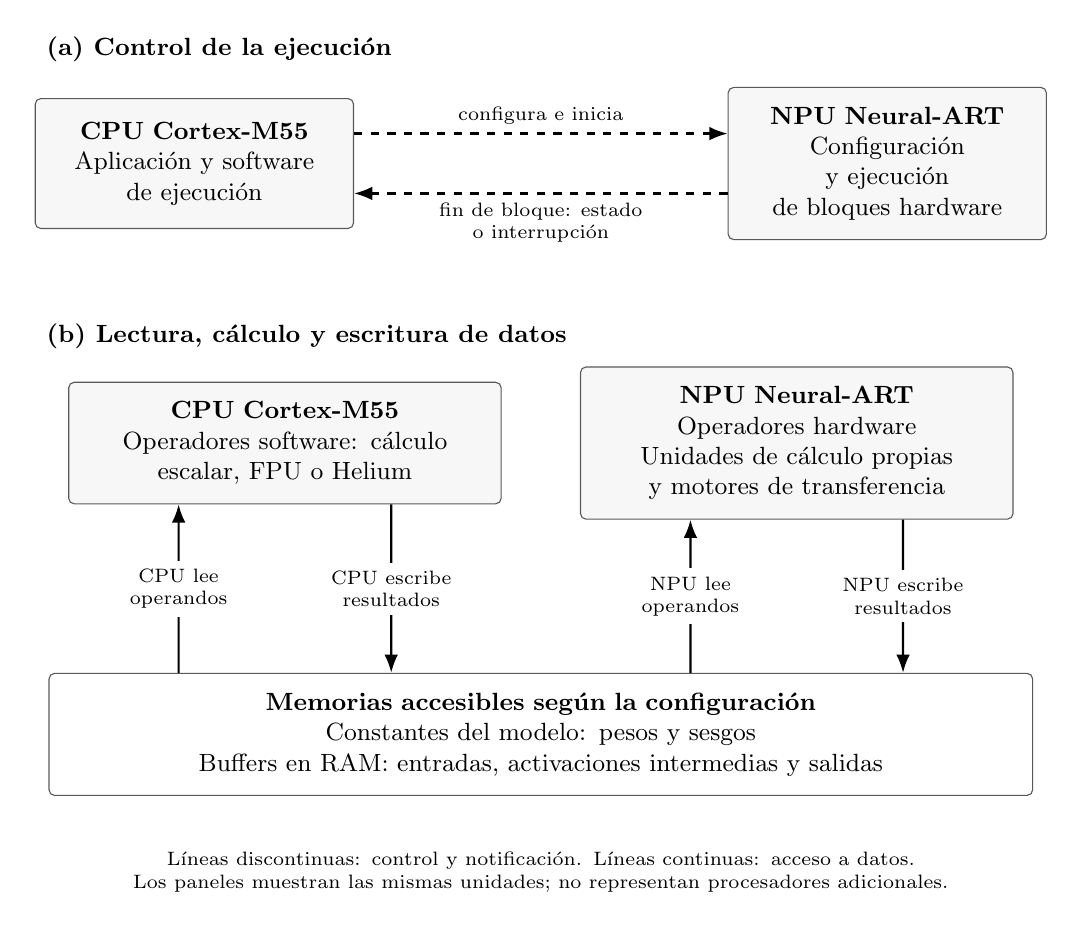
\begin{tikzpicture}[>=Latex,
 box/.style={draw=black!65,rounded corners=2pt,align=center,font=\small,inner sep=7pt},
 ctl/.style={->,thick,dashed},dat/.style={->,thick},
 lab/.style={font=\scriptsize,align=center,fill=white,inner sep=3pt}]
\node[anchor=west,font=\small\bfseries] at (-6.4,1.45) {(a) Control de la ejecución};
\node[box,text width=3.55cm,minimum height=1.65cm,fill=black!3] (cpuC) at (-4.4,0) {\textbf{CPU Cortex-M55}\\Aplicación y software\\de ejecución};
\node[box,text width=3.55cm,minimum height=1.65cm,fill=black!3] (npuC) at (4.4,0) {\textbf{NPU Neural-ART}\\Configuración y ejecución\\de bloques hardware};
\draw[ctl] ([yshift=0.38cm]cpuC.east) -- node[lab,above]{configura e inicia} ([yshift=0.38cm]npuC.west);
\draw[ctl] ([yshift=-0.38cm]npuC.west) -- node[lab,below]{fin de bloque: estado\\o interrupción} ([yshift=-0.38cm]cpuC.east);
\node[anchor=west,font=\small\bfseries] at (-6.4,-2.2) {(b) Lectura, cálculo y escritura de datos};
\node[box,text width=5.0cm,minimum height=1.3cm,fill=black!3] (cpuD) at (-3.25,-3.55) {\textbf{CPU Cortex-M55}\\Operadores software: cálculo\\escalar, FPU o Helium};
\node[box,text width=5.0cm,minimum height=1.3cm,fill=black!3] (npuD) at (3.25,-3.55) {\textbf{NPU Neural-ART}\\Operadores hardware\\Unidades de cálculo propias\\y motores de transferencia};
\node[box,text width=12.0cm,minimum height=1.55cm] (mem) at (0,-7.25) {\textbf{Memorias accesibles según la configuración}\\Constantes del modelo: pesos y sesgos\\Buffers en RAM: entradas, activaciones intermedias y salidas};
\draw[dat] ([xshift=-4.6cm]mem.north) -- node[lab,text width=1.95cm]{CPU lee\\operandos} ([xshift=-1.35cm]cpuD.south);
\draw[dat] ([xshift=1.35cm]cpuD.south) -- node[lab,text width=1.95cm]{CPU escribe\\resultados} ([xshift=-1.9cm]mem.north);
\draw[dat] ([xshift=1.9cm]mem.north) -- node[lab,text width=1.95cm]{NPU lee\\operandos} ([xshift=-1.35cm]npuD.south);
\draw[dat] ([xshift=1.35cm]npuD.south) -- node[lab,text width=1.95cm]{NPU escribe\\resultados} ([xshift=4.6cm]mem.north);
\node[font=\scriptsize,align=center,text width=12.8cm] at (0,-9.0) {Líneas discontinuas: control y notificación. Líneas continuas: acceso a datos.\\Los paneles muestran las mismas unidades; no representan procesadores adicionales.};
\end{tikzpicture}
\caption{Relación funcional entre CPU, NPU y memorias. Cada unidad realiza el cálculo que le corresponde; los búferes permiten intercambiar resultados. Esquema de elaboración propia basado en ST \cite{cap4_stconcepts}. Se omiten buses y cachés para destacar las funciones, sin suponer que todas las memorias tengan igual acceso o latencia.}\label{fig:hw}
\end{figure}

La Figura~\ref{fig:hw} separa dos relaciones. El \emph{control} indica quién configura e inicia el trabajo y cómo se reconoce su finalización; el \emph{flujo de datos} muestra quién lee los operandos y dónde escribe los resultados. Así, una orden de la CPU no representa el envío de cada multiplicación a través de Helium. La NPU accede a los búferes asignados y calcula con sus unidades; la CPU accede a memoria para ejecutar la aplicación y los operadores software \cite{cap4_stconcepts}.

\subsection{Cortex-M55 y tecnología MVE/Helium}\label{sec:cap4_helium}
\subsubsection{Procesamiento escalar, punto flotante y procesamiento vectorial}
Una instrucción escalar opera sobre valores individuales. En un producto interno, su implementación puede recorrer los datos y acumular un producto en cada paso. Una instrucción vectorial expresa operaciones sobre varios elementos agrupados, reduciendo la cantidad de instrucciones necesarias para describir determinados cálculos repetitivos. Esta organización se conoce como SIMD, del inglés \textit{Single Instruction, Multiple Data}.

La guía oficial de Arm proporciona la base conceptual de esta sección \cite{cap4_armcomplete}. Helium es el nombre de la extensión MVE, \textit{M-Profile Vector Extension}, de la arquitectura Armv8.1-M. Su propósito es favorecer cargas de procesamiento digital de señales y aprendizaje automático en microcontroladores \cite{cap4_armoverview}. El número de elementos de un vector depende de su representación numérica. Por ello, el cambio de Float32 a INT8 puede modificar tanto el almacenamiento como la forma de organizar las operaciones.

La unidad de punto flotante, o FPU, permite operar con números flotantes, pero una instrucción flotante puede ser escalar o vectorial. Para diferenciarlas se examinan el mnemónico y los registros utilizados. Las designaciones \texttt{S} y \texttt{Q} proceden de la nomenclatura de Arm: el manual técnico del Cortex-M55, Secciones~3.4 y~14.1.1, identifica \texttt{S0--S31} como 32 registros de una palabra de 32 bits y \texttt{Q0--Q7} como ocho registros vectoriales de 128 bits. Son vistas de un mismo banco de registros de extensión \cite{cap4_armtrm}.

En una operación escalar Float32, un registro \texttt{S} contiene un valor de precisión simple. Un registro \texttt{Q} agrupa varios elementos, por ejemplo cuatro Float32 o dieciséis INT8. Las letras minúsculas \texttt{s} y \texttt{q} de los listados son la escritura de esas designaciones en el desensamblado. Por tanto, las instrucciones \texttt{vmul.f32} y \texttt{vfma.f32} con operandos \texttt{s} de la Sección~\ref{sec:cap4_evidencia} corresponden a cálculo flotante escalar; la interpretación vectorial requiere identificar una instrucción MVE y sus operandos. Esto no significa que todo registro escalar se denomine \texttt{S}: Arm también define registros generales \texttt{R} \cite{cap4_armtrm}.

\subsubsection{Registros, vectores, elementos y carriles}
Un \emph{registro} es un espacio de almacenamiento de acceso inmediato para las instrucciones del procesador. En MVE, un registro vectorial contiene 128 bits. Un \emph{vector} es el conjunto de valores contenidos en ese registro y cada valor es un \emph{elemento}. El \emph{carril}, o \textit{lane}, identifica una posición correspondiente entre los vectores sobre los que se realiza una operación \cite{cap4_armregisters}.

La Tabla~\ref{tab:cap4_vectores} relaciona el ancho de cada elemento con el número de posiciones del registro. Los 128 bits se mantienen; cambia su interpretación. Cuatro valores Float32 y dieciséis valores INT8 ocupan, respectivamente, un registro vectorial completo. La existencia de dieciséis posiciones INT8 no implica que toda instrucción termine en un ciclo ni garantiza una aceleración de dieciséis veces: el tiempo también depende de las cargas, los almacenamientos, las dependencias y la implementación de cada instrucción.

\begin{table}[H]\centering\small
\caption{Organización de un registro MVE de 128 bits para los formatos de interés. Elaboración a partir de la documentación de Arm \cite{cap4_armregisters}.}\label{tab:cap4_vectores}
\begin{tabularx}{\linewidth}{lccY}\toprule
Formato & Bits por elemento & Elementos & Ejemplo de utilización\\\midrule
INT8 & 8 & 16 & Pesos o activaciones cuantizados.\\
INT16 & 16 & 8 & Señales enteras de mayor resolución.\\
INT32 & 32 & 4 & Resultados enteros de mayor anchura.\\
Float32 & 32 & 4 & Valores de punto flotante.\\\bottomrule
\end{tabularx}
\end{table}

Como ejemplo conceptual, al sumar dos vectores de cuatro elementos, la posición cero del primer vector se suma con la posición cero del segundo y el resultado se almacena en la posición cero del destino. Las demás posiciones siguen la misma regla. Si una capa contiene más elementos que los disponibles en un registro, el cálculo se organiza por bloques sucesivos.

\subsubsection{Predicación y tratamiento del último bloque}
La \emph{predicación} permite seleccionar qué posiciones participan en una operación vectorial. Una máscara indica los elementos activos y los inactivos. Arm describe variantes que conservan un valor previo, asignan cero o dejan sin especificar el contenido de las posiciones inactivas, según la operación \cite{cap4_armpredication}.

Considérese una operación sobre 18 valores INT8. Un bloque puede procesar los primeros 16 y un segundo bloque contiene solamente dos valores válidos. La máscara de predicación del segundo bloque habilita esas dos posiciones. Las restantes se tratan conforme a la semántica de la instrucción, evitando que contribuyan indebidamente al resultado o que se realicen accesos no válidos. Este mecanismo permite manejar longitudes que no son múltiplos del número de elementos del vector.

En el código ensamblador, instrucciones como \texttt{vctp.8} crean un predicado según la cantidad de elementos de ocho bits pendientes; \texttt{vpst} introduce la predicación de las instrucciones vectoriales siguientes. En un desensamblado, su presencia junto con cargas vectoriales permite reconocer el tratamiento de bloques y de sus elementos finales. En este contexto, un intrínseco es una función reconocida por el compilador que permite expresar una operación específica del procesador. Las extensiones de lenguaje de Arm proporcionan intrínsecos para expresar estas operaciones desde C o C++ \cite{cap4_acle}.

\subsubsection{Multiplicación y acumulación: VMLA y VMLADAVA}
La multiplicación y acumulación aparece de forma recurrente en capas densas y convolucionales. Sin embargo, existen instrucciones que conservan un resultado por posición e instrucciones que reúnen varios productos en un resultado escalar. Distinguirlas permite relacionar el código máquina con el cálculo de una neurona.

En el ejemplo \texttt{VMLA} presentado por Arm, un vector se multiplica por un escalar y se suma al vector acumulador \cite{cap4_armvmla}. Su efecto puede escribirse como
\begin{equation}
d_i^{\mathrm{nuevo}}=d_i^{\mathrm{previo}}+a_i\,c,
\qquad i=0,\ldots,L-1,
\label{eq:cap4_vmla}
\end{equation}
donde $L$ es el número de elementos, $a_i$ pertenece al vector de entrada, $c$ es un escalar y $d_i$ es cada elemento del acumulador. Para el ejemplo didáctico $d=[1,1,1,1]$, $a=[2,3,4,5]$ y $c=2$, el resultado es $[5,7,9,11]$. Se conservan cuatro resultados, uno por posición.

La operación descrita mediante \texttt{VMLADAV} multiplica elementos correspondientes y suma los productos para producir un escalar. \texttt{VMLADAVA} añade ese resultado al valor previo del acumulador escalar \cite{cap4_armvmladava}:
\begin{equation}
A_{\mathrm{nuevo}}=A_{\mathrm{previo}}+\sum_{i=0}^{L-1}a_iw_i.
\label{eq:cap4_vmladava}
\end{equation}
La suma entre posiciones se denomina \emph{reducción}. Por ejemplo, con $a=[1,2,3,4]$, $w=[2,-1,0,3]$ y $A_{\mathrm{previo}}=5$, la suma de productos es $2-2+0+12=12$ y el acumulador final vale 17. Esta forma de cálculo coincide con la estructura de un producto interno, aunque una capa completa también requiere sesgo, escalado y activación.

Las Ecuaciones~\ref{eq:cap4_vmla} y \ref{eq:cap4_vmladava} expresan el comportamiento conceptual descrito por Arm, suponiendo que no existe desbordamiento. Los anchos de operandos y acumuladores, así como las variantes disponibles, dependen de la instrucción concreta. Los nombres encontrados en el binario se conservan tal como aparecen; no se sustituye un mnemónico observado por el utilizado en un ejemplo teórico.

\subsubsection{Bibliotecas de inferencia y utilización efectiva de Helium}
Las instrucciones vectoriales pueden incorporarse mediante código ensamblador, intrínsecos o transformaciones del compilador. Una biblioteca de inferencia organiza estos recursos en rutinas para convoluciones, capas densas y otras operaciones. CMSIS-NN ofrece implementaciones destinadas a distintos grupos de Cortex-M, incluidas variantes para procesadores con MVE; la selección depende de las características habilitadas al compilar \cite{cap4_cmsisnn}.

En esta memoria, la presencia de Helium se estudia en las funciones enlazadas al firmware. El tipo numérico del modelo constituye un antecedente, pero no demuestra qué instrucciones se generaron. Una implementación Float32 puede contener cálculo escalar o vectorial, y una INT8 puede combinar rutinas vectoriales con código escalar de control. La evidencia debe asociarse con funciones concretas y con su relación con la red.

\subsection{Organización y funcionamiento de Neural-ART}\label{sec:cap4_neuralart}
\subsubsection{Unidades especializadas y flujo de datos}
Neural-ART es un acelerador de inferencia reconfigurable. La configuración Neural-ART 14 integrada en STM32N6 reúne unidades de convolución, activación, aritmética y agrupamiento, conectadas mediante un flujo de datos. Los motores de transferencia, o \textit{stream engines}, suministran operandos y escriben resultados en memoria. Una vez iniciada una configuración, el acelerador realiza su procesamiento sin que la CPU ejecute cada multiplicación \cite{cap4_stconcepts}.

La Tabla~\ref{tab:cap4_unidades} presenta sus componentes principales. El agrupamiento, o \textit{pooling}, reduce una región mediante operaciones como máximo o promedio. Las operaciones elemento a elemento actúan sobre posiciones correspondientes de los tensores. La convolución combina regiones de entrada con filtros, mientras que la activación aplica la transformación no lineal requerida por la red.

\begin{table}[H]\centering\small
\caption{Unidades de procesamiento de Neural-ART 14 descritas por ST \cite{cap4_stconcepts}.}\label{tab:cap4_unidades}
\begin{tabularx}{\linewidth}{lcY}\toprule
Unidad & Cantidad & Función principal\\\midrule
\texttt{CONV\_\allowbreak ACC} & 4 & Cálculos de convolución mediante multiplicación y acumulación.\\
\texttt{POOL\_\allowbreak ACC} & 2 & Operaciones de agrupamiento.\\
\texttt{ACTIV\_\allowbreak ACC} & 2 & Funciones de activación.\\
\texttt{ARITH\_\allowbreak ACC} & 4 & Operaciones aritméticas y transformaciones afines.\\
\texttt{STREAM\_\allowbreak ENG} & 10 & Lectura y escritura de flujos de datos; cinco por puerto.\\\bottomrule
\end{tabularx}
\end{table}

Puede entenderse el procesamiento mediante una cadena conceptual: se leen las activaciones y los pesos, se calculan las sumas ponderadas y se aplican las transformaciones necesarias para producir la salida. El compilador adapta esa cadena a los recursos disponibles. La ubicación de los datos influye en cuánto tiempo se tarda en alimentar las unidades, por lo que disponer de capacidad aritmética no garantiza que ésta permanezca ocupada durante toda la inferencia.

Para el clasificador de radiografías, las convoluciones concentran operaciones repetidas sobre mapas de características. En la red MPC, las capas densas calculan productos entre matrices de pesos y vectores de estado o activaciones. En ambos casos importa el \emph{tamaño de los tensores}: sus dimensiones determinan cuántos datos deben almacenarse y transferirse, así como la cantidad y organización del cálculo. Por ejemplo, un mapa hipotético de $32\times32\times16$ contiene 16\,384 elementos: ocupa 16\,384 bytes en INT8 y 65\,536 bytes en Float32, antes de considerar alineamiento u otros búferes. Este ejemplo ilustra almacenamiento de datos, no memoria total del firmware.

Un tensor pequeño puede ofrecer poco trabajo para ocupar las unidades paralelas y amortizar la preparación de un bloque. Uno mayor puede proporcionar más paralelismo, pero también exigir más transferencias o particiones si supera la memoria disponible. Por ello, ``mayor tamaño'' no equivale automáticamente a ``mayor aceleración''. Sze et al. explican que las dimensiones de las capas, su asignación a las unidades de procesamiento y la reutilización de datos condicionan el aprovechamiento del hardware y los accesos a memoria \cite{cap4_sze2017}; ST describe estos límites de cómputo y memoria específicamente para Neural-ART \cite{cap4_stconcepts}.

La \emph{continuidad de las regiones} se refiere a una sucesión de operaciones conectadas en el grafo que puede permanecer en la NPU, sin intercalar un operador que deba calcular la CPU. No significa contigüidad de direcciones de memoria. Como ejemplo conceptual, una convolución, su activación y un agrupamiento compatibles pueden formar una región acelerada. Si entre dos regiones aparece un cálculo Float32, es necesario hacer disponible el resultado para la CPU y posteriormente para la NPU; según los formatos, también se requieren conversiones. Estas fronteras añaden trabajo de coordinación y pueden limitar el beneficio global. Chen et al. analizan cómo la agrupación de operadores reduce accesos intermedios y costos de invocación \cite{cap4_tvm2018}; para Neural-ART, las rutas software y la agrupación de épocas se rigen por el modelo de ejecución de ST \cite{cap4_stconcepts}. Una región continua puede abarcar varias épocas y no implica que todos sus resultados permanezcan dentro de las unidades aritméticas.

\subsubsection{Épocas de ejecución y coordinación con la CPU}
El grafo puede superar los recursos que la NPU utiliza simultáneamente. El compilador lo divide entonces en unidades de ejecución denominadas \emph{épocas}. En este contexto, una época es un bloque del programa de inferencia y no una pasada de entrenamiento sobre el conjunto de datos.

ST distingue épocas hardware, software e híbridas, además de metaépocas que agrupan secuencias hardware bajo el controlador de épocas. Las primeras ejecutan el cálculo asignado en Neural-ART; las software utilizan el procesador anfitrión; las híbridas combinan intervención de software y recursos hardware \cite{cap4_stconcepts}. Esta terminología permite describir el reparto del procesamiento sin reducirlo a una etiqueta única para toda la red.

Una \emph{dependencia de datos} aparece cuando una operación necesita el resultado de otra. Por ejemplo, si una capa densa produce un vector y la siguiente aplica una activación a ese vector, esta última necesita los valores calculados por la primera. El orden de ejecución debe asegurar que los datos requeridos estén disponibles antes de consumirlos. Esto también ocurre si la capa densa se asigna a la NPU y la activación a la CPU: cambiar de procesador no elimina la dependencia.

ST establece un orden fijo de épocas para preservar esas relaciones en el grafo. El entorno de ejecución prepara un bloque, inicia su procesamiento y comprueba la finalización de sus transferencias antes de cerrar la etapa. Los resultados que deben persistir entre épocas se conservan en el subsistema de memoria externo a las unidades de cálculo de la NPU; esta expresión puede incluir SRAM interna del microcontrolador y no implica necesariamente memoria fuera del chip. Dentro de una época pueden existir unidades conectadas por flujos de datos, por lo que esta explicación no presupone un almacenamiento completo entre cada par de operadores \cite{cap4_stconcepts}.

El controlador de épocas puede ejecutar una secuencia de configuraciones hardware generada previamente, reduciendo la intervención de la CPU entre esos bloques. La CPU sigue gestionando la aplicación y los bloques software. Es útil distinguir \emph{coordinar} una operación de \emph{calcularla}: iniciar la NPU desde Cortex-M55 no significa que Cortex-M55 efectúe sus productos y sumas. Cuando el compilador asigna un operador a Neural-ART, el cálculo se realiza en sus unidades especializadas; cuando genera una ruta software, el entorno de ejecución invoca una función en Cortex-M55, que puede emplear Helium si su implementación está vectorizada \cite{cap4_stconcepts,cap4_cmsisnn}.

En consecuencia, encontrar instrucciones MVE en un firmware que también utiliza la NPU evidencia código destinado a la CPU. Ese código puede corresponder a un operador software, una conversión u otra tarea. No demuestra que una operación ya asignada a las unidades aritméticas de Neural-ART se ejecute mediante Helium. El reparto se establece en el código y las configuraciones generados por el compilador, y su ejecución se comprueba con los perfiles; el acelerador no decide trasladar cada multiplicación a la CPU durante la inferencia \cite{cap4_stconcepts,cap4_stcompiler}.

\subsection{Compilación y compatibilidad de operadores}\label{sec:cap4_compilacion}
\subsubsection{Del modelo convertido a la implementación ejecutable}
El modelo exportado describe operadores, conexiones y parámetros numéricos. Para ejecutarlo en la placa, la cadena de herramientas transforma esa descripción en código, datos y configuraciones adaptados al destino. El compilador de Neural-ART utiliza una descripción del acelerador, las propiedades del procesador anfitrión y los pools de memoria disponibles. En el flujo documentado por ST, las representaciones intermedias ONNX y JSON transportan el grafo y su información de cuantización \cite{cap4_stcompiler}.

Durante este proceso pueden reorganizarse operaciones, combinarse transformaciones y generarse buffers que no coinciden uno a uno con los tensores originales. Por ello, una capa del modelo de alto nivel no tiene que corresponder a una única época ni a una única función del binario. La interpretación experimental debe relacionar el modelo de entrada, la representación generada y el perfil de ejecución.

La asignación depende tanto del operador como de sus dimensiones, parámetros y tipo numérico. Una convolución puede ser compatible en una configuración y requerir una descomposición o una ruta software en otra. La compilación satisfactoria demuestra que se obtuvo una implementación; comprobar su precisión efectiva y sus resultados exige revisar los artefactos generados y validar la inferencia.

\subsubsection{Formatos admitidos y alcance de la compatibilidad}
La compatibilidad se determina por el conjunto formado por operador, dimensiones, parámetros y representación numérica. La Sección \emph{Inference Model Constraints} de ST Edge AI Core 4.0.1 establece las siguientes condiciones para el flujo Neural-ART \cite{cap4_stoperators}:
\begin{enumerate}
\item \textbf{Solo inferencia.} La NPU ejecuta redes ya preparadas; no dispone de un modo de entrenamiento.
\item \textbf{Formas estáticas.} Las dimensiones de entrada y salida deben quedar definidas al compilar. Son sus tamaños los que permanecen fijos, no los valores de cada muestra.
\item \textbf{Lote variable interpretado como uno.} Una dimensión de lote declarada como \texttt{None} se considera de tamaño 1 en este flujo.
\item \textbf{Conectividad válida.} No se admite un operador cuya salida esté sin conectar en la representación del grafo presentada al compilador.
\item \textbf{Operandos cuantizados.} Un operador híbrido, por ejemplo con pesos INT8 y activaciones Float32, no tiene asignación directa a la NPU; ambos deben estar cuantizados.
\item \textbf{Formato INT8.} Para pesos y activaciones se especifica INT8 con escala y punto cero, bajo el esquema \texttt{ss/sa} y las reglas por canal correspondientes.
\item \textbf{Float32 en software.} Una operación solicitada en Float32 se asigna al procesador anfitrión.
\end{enumerate}

La notación \texttt{ss/sa} identifica pesos con signo y cuantización simétrica, y activaciones con signo y cuantización asimétrica. ST distingue la escala por canal de los pesos, en los operadores que la emplean, de la escala por tensor de las activaciones; no significa que cada activación tenga su propia escala \cite{cap4_stquant}. La restricción sobre operadores híbridos tampoco equivale a prohibir un \emph{modelo de precisión mixta}: este puede combinar operadores INT8 completos con otros Float32 separados. Los primeros son candidatos a la NPU si cumplen las demás condiciones; los segundos se ejecutan en CPU, con conversiones en las fronteras que las requieran \cite{cap4_stoperators,cap4_stquant}.

Estas condiciones permiten anticipar la dificultad de INT16$\times$8: aunque sus pesos sean INT8, sus activaciones INT16 no satisfacen el esquema de ocho bits para ambos tensores que requiere la asignación directa descrita. Esta observación identifica una incompatibilidad con el flujo documentado, pero no determina por sí sola qué transformación realizará el compilador en cada modelo. Esa transformación se establece mediante los informes y el código generado.

Debe distinguirse, además, el formato que admite el compilador de los anchos internos del circuito. ST describe rutas enteras de 8, 16 y 24 bits y multiplicaciones de $16\times16$ bits en Neural-ART \cite{cap4_stconcepts}. La presencia de esos recursos físicos no implica que el flujo TFLite INT16$\times$8 esté implementado: también se necesitan las reglas de escalado, los operadores y las transformaciones que permitan asignar ese modelo al hardware. En consecuencia, la compatibilidad se atribuye a la variante y a la versión de herramientas utilizadas, mientras que su representación efectiva después de compilar se verifica experimentalmente.

\begin{table}[H]\centering\small
\caption{Ejemplos de asignación de operadores TensorFlow Lite en ST Edge AI Core 4.0.1. La ruta hardware supone una configuración cuantizada compatible \cite{cap4_stoperators}.}\label{tab:cap4_operadores}
\begin{tabularx}{\linewidth}{p{3.5cm}lY}\toprule
Operador & Ruta documentada & Consideración\\\midrule
\texttt{CONV\_\allowbreak 2D} & HW & Pesos constantes y restricciones de configuración.\\
\texttt{FULLY\_\allowbreak CONNECTED} & HW & Parámetros y tensores compatibles.\\
\texttt{RELU}, \texttt{TANH} & HW & Su nombre no obliga a ejecutarlos en CPU; importa su representación.\\
\texttt{MAX\_\allowbreak POOL\_\allowbreak 2D} & HW & Puede requerir descomposición según la ventana.\\
\texttt{SOFTMAX} & HW o SW & Hardware con \texttt{--expand-softmax}; software entero en caso contrario.\\
\texttt{QUANTIZE}, \texttt{DEQUANTIZE} & SW Float32 & Fronteras entre punto flotante y enteros.\\\bottomrule
\end{tabularx}
\end{table}

La presencia de \texttt{TANH} en la red MPC no implica por sí misma un fallback: su variante cuantizada aparece en el soporte hardware publicado. Si una activación se preserva en Float32 o forma parte de una región que no cumple las condiciones de asignación, su ejecución debe interpretarse conforme a esa configuración. Esta precisión evita atribuir una limitación al nombre de la función cuando el factor determinante es su representación o su contexto.

\subsection{Memoria, transferencias y coherencia de datos}\label{sec:cap4_memoria}
Los pesos son parámetros de la red; las activaciones son resultados que cambian con cada entrada. Ambos deben estar accesibles para la unidad que los consume. Un \emph{pool de memoria} describe una región disponible y sus propiedades, como dirección, tamaño, latencia y capacidad de transferencia. El compilador utiliza esa información para ubicar buffers y constantes \cite{cap4_stcompiler}.

En los experimentos de esta memoria se conservó la asignación generada por las herramientas para cada modelo. La memoria reportada depende de esa asignación y de las transformaciones de compilación. El tamaño serializado de un archivo \texttt{.tflite} y el almacenamiento de su implementación compilada son magnitudes distintas: el firmware incorpora código, constantes, alineamientos y estructuras de ejecución.

La caché conserva copias de datos para reducir determinados accesos a memoria. Cuando CPU y NPU intercambian buffers, esas copias deben corresponder a los datos válidos. Una limpieza de caché, o \textit{clean}, escribe datos modificados hacia la memoria correspondiente; una invalidación descarta copias para que no se reutilice información desactualizada. La documentación del compilador contempla la generación de mantenimiento de caché para las regiones compartidas \cite{cap4_stcompiler}.

Este mantenimiento tiene una función de corrección, además de un costo temporal. En los extractos experimentales de la Sección~\ref{sec:cap4_evidencia} aparecen llamadas a rutinas de invalidación y limpieza alrededor de operaciones software. Su presencia evidencia que la implementación generada incluye esa coordinación; no permite deducir por sí sola toda la configuración de caché ni su contribución temporal.

\subsection{Fallback y relación con las estrategias de cuantización}\label{sec:cap4_fallback}
\subsubsection{Fallback de procesamiento y cambio de representación}
Un \emph{fallback} es una ruta alternativa utilizada cuando una operación no se asigna a la implementación inicialmente prevista. En el flujo de Neural-ART, ST documenta alternativas asistidas por hardware, rutinas enteras en software y rutinas flotantes con conversiones cuando corresponde. Si no existe una implementación admisible, la generación puede terminar con un error \cite{cap4_stconcepts}.

Resulta útil distinguir dos efectos. El primero es un cambio de unidad de procesamiento: una operación INT8 puede ejecutarse en Cortex-M55 mediante una rutina entera. El segundo es un cambio de representación: el cálculo puede realizarse en Float32, con las conversiones necesarias en sus fronteras. La ejecución en CPU no implica automáticamente punto flotante, y la existencia de datos INT8 no implica automáticamente ejecución en NPU.

En una red de precisión mixta, preservar deliberadamente regiones Float32 introduce una decisión adicional. Su cálculo software responde a la representación seleccionada para conservar fidelidad numérica. El análisis debe distinguir esas regiones de las operaciones que permanecen cuantizadas pero requieren CPU por restricciones del compilador o del operador.

\subsubsection{INT16x8: fidelidad numérica y representación desplegada}
El estudio del controlador identificó INT16$\times$8 como una alternativa de interés en simulación, al ofrecer mayor resolución para las activaciones que INT8. Sin embargo, en el despliegue evaluado en este trabajo, los informes de generación identifican una representación flotante y el código inspeccionado es consistente con cálculo Float32 en Cortex-M55. Este resultado corresponde a la implementación obtenida con la cadena de herramientas utilizada y se desarrolla cuantitativamente en el capítulo de resultados.

Por ello, esa ejecución no constituye una evaluación de inferencia nativa INT16$\times$8 sobre Neural-ART. Tampoco debe interpretarse el cambio de tipo como una recuperación automática de los pesos originales: reconstruir en Float32 un parámetro previamente cuantizado conserva la aproximación introducida por la cuantización. La precisión aritmética del firmware y la fidelidad respecto del modelo de referencia son propiedades que se comprueban por separado.

El hallazgo motiva evaluar una alternativa que mantenga parte del procesamiento cuantizado después de compilar. La conclusión no se obtiene únicamente del formato del archivo exportado, sino de la representación generada y de la ejecución observada en la plataforma.

\subsubsection{Justificación de la precisión mixta selectiva}
La precisión mixta selectiva conserva una base INT8 y mantiene determinadas regiones sensibles en Float32. Desde el punto de vista numérico, busca reducir perturbaciones que afectan el comportamiento del controlador. Desde el punto de vista de implementación, permite conservar regiones compatibles con el flujo INT8 de Neural-ART mientras otras se ejecutan en software.

La relación con INT16$\times$8 es funcional: ambas estrategias buscan evitar que la pérdida de resolución deteriore el control, mediante decisiones numéricas diferentes. La precisión mixta no reproduce necesariamente sus valores internos ni garantiza las mismas trayectorias. Su utilidad se determina mediante la evaluación en lazo cerrado y la verificación del formato efectivo de la implementación.

Las regiones Float32 se ejecutan en CPU según el soporte documentado por ST \cite{cap4_stoperators}. Cada frontera efectiva INT8/Float32 requiere adaptar los datos entre representaciones. Si se preservan demasiadas regiones o se fragmenta el cálculo en bloques pequeños, las conversiones, las transferencias y la coordinación pueden reducir la ganancia de aceleración. La selección implementada se basa en el diagnóstico de error numérico y en reglas explícitas de conservación de capas; su costo de ejecución se evalúa posteriormente. El indicador utilizado es una heurística y no acredita por sí solo sensibilidad funcional. La aceptación del controlador requiere comprobar las exigencias del ensayo: seleccionar una alternativa para investigarla no implica que ya las satisfaga en todas las condiciones.

\subsection{Interpretación de los perfiles y relación con los resultados}\label{sec:cap4_perfiles}
La documentación del perfilador de ST distingue la duración de cada época, sus fases de preparación y finalización, los ciclos de la CPU y los ciclos del núcleo NPU. También presenta indicadores para la ejecución completa \cite{cap4_stprofiler}. Esta separación permite diferenciar tiempo de cálculo acelerado, operaciones software y sobrecarga de coordinación.

Como descripción contable de una ejecución secuencial, el tiempo de inferencia puede escribirse como
\begin{equation}
T_{\mathrm{inf}}=T_{\mathrm{inicio}}+\sum_{j=1}^{E}T_j+T_{\mathrm{cierre}},
\label{eq:cap4_tiempo}
\end{equation}
donde $E$ es el número de bloques considerados y cada $T_j$ incluye todas las fases de ese bloque, contabilizadas una sola vez. Esta expresión organiza las mediciones y no presupone que toda la duración de una época hardware corresponda a multiplicaciones útiles. Si el instrumento ya incluye preparación y cierre dentro de su duración total, esos intervalos no deben sumarse nuevamente.

El número de épocas hardware tampoco equivale a la fracción temporal acelerada: un bloque puede concentrar la mayor parte del cálculo, mientras otros realizan operaciones breves. Del mismo modo, la latencia de inferencia debe distinguirse del tiempo de intercambio por UART. En el banco de control, el tiempo de respuesta del sistema incluye además comunicación, procesamiento de entradas y entrega de la acción a la simulación.

La selección de una variante se apoya así en tres evidencias complementarias: el modelo convertido describe la representación numérica propuesta; el código y los informes de compilación muestran su implementación; las pruebas en placa y en lazo cerrado establecen su costo y su comportamiento funcional. El estudio de Helium, Neural-ART y los fallbacks permite interpretar por qué una alternativa favorable en simulación puede cambiar al desplegarse y por qué la precisión mixta selectiva requiere analizar conjuntamente fidelidad y ejecución efectiva.


\chapter{Estado del arte}\label{cap:estado}
La revisión se concentra en trabajos que estudian la reducción de precisión de redes neuronales, la aproximación de controladores predictivos y su implementación en sistemas embebidos. El propósito es identificar qué resuelven estos antecedentes y qué aspectos requieren evaluación en los dos casos de esta memoria: clasificación de radiografías y control del cartpole mediante una red que aproxima una política MPC. La comparación permite formular una brecha de evaluación e implementación, sin atribuir novedad a los formatos numéricos utilizados.

\section{Cuantización de redes: calidad de tarea y costo de inferencia}
Jacob et al. proponen cuantizar pesos y activaciones a ocho bits y adaptar el entrenamiento para permitir inferencia con aritmética entera. Sus experimentos con clasificación ImageNet y detección COCO muestran un compromiso favorable entre calidad y latencia en CPU ARM \cite{jacob2018}. El trabajo establece una base para QAT y para evaluar conjuntamente el resultado predictivo y el costo de ejecución. Sin embargo, sus tareas y plataformas no permiten anticipar el comportamiento en lazo cerrado de un controlador cuantizado ni la asignación de operadores a Neural-ART.

Nagel et al. sistematizan procedimientos PTQ y QAT orientados a limitar la degradación introducida por la cuantización \cite{nagel2021}. Su análisis aporta criterios para comparar una conversión posterior al entrenamiento con otra que adapta los parámetros durante el entrenamiento. Para esta memoria, la consecuencia es metodológica: deben conservarse ambas alternativas como referencias y comprobar su desempeño en cada aplicación, en lugar de asumir que un procedimiento será siempre superior.

Li et al. presentan BRECQ, que reconstruye bloques de la red para reducir el error de PTQ e incorpora precisión mixta a partir de la sensibilidad de sus componentes. Lo evalúan en clasificación y detección \cite{brecq2021}. El antecedente respalda estudiar una asignación de precisión no uniforme, pero no demuestra que INT8 cause necesariamente inestabilidad o \emph{chattering} en un MPC. Tampoco equivale al procedimiento de esta memoria: conservar regiones seleccionadas en Float32 dentro de un modelo parcialmente INT8 no reproduce el algoritmo de reconstrucción ni la selección de anchos de bits de BRECQ.

Estos trabajos son directamente pertinentes al caso de radiografías como problema de clasificación sometido a compresión numérica. No constituyen una validación clínica del clasificador estudiado. Su utilidad reside en orientar la comparación de calidad de tarea, tamaño y costo de implementación; el comportamiento de la CNN concreta y de sus variantes debe establecerse con los datos y registros experimentales propios.

\section{MPC aproximado: del error de la red al comportamiento de control}
\subsection{Aproximación neuronal y adaptación de parámetros}
Hose, Gräfe y Trimpe desarrollan una arquitectura de MPC aproximado que utiliza sensibilidades para ajustar el controlador neuronal ante cambios conocidos de parámetros sin repetir todo el entrenamiento \cite{hose2024}. El repositorio asociado al trabajo presenta un flujo de generación de datos, entrenamiento y despliegue en STM32G4 para el levantamiento y la estabilización de un cartpole \cite{hoserepo}. Su contribución principal es la adaptación de la política aproximada, no una comparación de esquemas de cuantización sobre STM32N6.

Este trabajo es el antecedente del caso de control de la memoria, que examina los cambios de comportamiento al reducir la precisión de la representación neuronal y compilarla para otro destino. Utilizar ese antecedente no transfiere automáticamente sus garantías a una red convertida, cuantizada o ejecutada mediante una cadena de herramientas distinta. Por ello se requiere contrastar la concordancia de la acción calculada y el desempeño de las trayectorias en lazo cerrado.

\subsection{Compensación de una red cuantizada mediante LQR}
Sathyanarayanan et al. aproximan mediante una red neuronal el nivel de seguimiento de un MPC no lineal para invernaderos y cuantizan esa red. Añaden una acción LQR para compensar las desviaciones de la aproximación cuantizada \cite{greenhouse2024}. En el escenario presentado, la red cuantizada sin compensación exhibe desviaciones de estado y una vulneración de la restricción de CO$_2$; la compensación mejora el seguimiento en gran parte del ensayo. El trabajo muestra así que una implementación compacta y rápida puede necesitar una evaluación funcional adicional.

La implementación utiliza un STM32F407 con Cortex-M4F a 168 MHz. Los autores informan una red de aproximadamente 3800 parámetros, menos de 5 kB de Flash para almacenar sus parámetros cuantizados y la información adicional de cuantización, y una inferencia media cercana a 200~$\mu$s para la red. El almacenamiento descrito no equivale a la ocupación total del firmware, ni la inferencia al ciclo completo de control. Estas cifras corresponden a su aplicación y no son directamente intercambiables con las del cartpole. Las garantías consideradas para el LQR no se extienden automáticamente al funcionamiento con saturación, y esta compensación no impone por sí misma las restricciones de estado.

La relación con esta memoria es precisa: ese antecedente modifica la ley de control agregando compensación, mientras que aquí se estudia si una mayor resolución numérica o la conservación selectiva de regiones Float32 mejora la fidelidad del controlador neuronal. Se trata de una alternativa que debe evaluarse, no de una demostración previa de que puede sustituir al LQR. El problema descrito en el artículo es la degradación de seguimiento y restricciones; no se utiliza como prueba de que la compensación elimine universalmente el \emph{chattering}.

\section{Precisión mixta y mayor resolución como alternativas}
\subsection{Precisión mixta en MPC explícito robusto}
Salamati et al. estudian implementaciones de precisión mixta para MPC explícito robusto de sistemas lineales invariantes en el tiempo \cite{salamati2019}. El controlador se representa mediante regiones poliédricas y leyes afines, y el procedimiento ajusta la precisión manteniendo el error dentro del margen de robustez considerado. En sus bancos de prueba, informan una reducción de almacenamiento de hasta 20,9\% y de 12,6\% en promedio frente a una implementación de precisión uniforme mínima.

El aporte relevante es que la precisión puede asignarse de forma no uniforme atendiendo a restricciones de error y recursos. No obstante, su representación no es una red neuronal, y sus garantías provienen de un análisis específico del controlador robusto. La selección de regiones Float32 realizada en esta memoria no reproduce ese análisis ni hereda sus garantías. Por tanto, Salamati aporta la motivación para estudiar precisión mixta bajo restricciones funcionales, mientras que el antecedente de red cuantizada con compensación LQR corresponde al trabajo de invernaderos.

\subsection{INT16x8 y precisión mixta selectiva en la red neuronal}
La documentación de LiteRT describe INT16x8 como una representación con activaciones enteras de 16 bits y pesos de ocho bits. La presenta como una opción para modelos cuyas activaciones son sensibles a la cuantización \cite{litert16}. Esta fuente es un antecedente de implementación, no un estudio que demuestre estabilidad de un MPC. La disponibilidad de la conversión tampoco garantiza que un compilador o acelerador concreto ejecute nativamente ese formato.

A partir de los antecedentes anteriores se plantean dos respuestas distintas a la pérdida de fidelidad. INT16x8 aumenta la resolución de las activaciones manteniendo pesos compactos; la precisión mixta selectiva conserva regiones Float32 y cuantiza otras a INT8. La primera explora un cambio de representación numérica; la segunda, una asignación no uniforme dentro del grafo. Su motivación común es reducir la perturbación introducida por la cuantización sin volver necesariamente a una implementación completamente Float32.

El interés de evaluarlas no presupone que sean más rápidas ni que siempre recuperen el comportamiento de referencia. La mayor precisión puede aumentar memoria y tiempo, y la mezcla de tipos puede introducir conversiones o ejecución software. La contribución experimental consiste en determinar qué parte de la ventaja observada en el modelo convertido se mantiene después de la compilación y durante la aplicación.

\section{Evaluación embebida y síntesis de los antecedentes}
Banbury et al. proponen MLPerf Tiny para comparar inferencia embebida mediante calidad de tarea, latencia y energía con procedimientos reproducibles \cite{banbury2021}. El antecedente refuerza la necesidad de evaluar el sistema ejecutado, no sólo el tamaño del archivo o el error calculado en el computador. Esta memoria adopta ese criterio de trazabilidad, pero no constituye una ejecución oficial de MLPerf Tiny ni incluye mediciones de energía.

La Tabla~\ref{tab:estado} resume los antecedentes más próximos a la pregunta de investigación. Las diferencias indicadas delimitan su relación con esta memoria; no implican deficiencias de los objetivos originales de cada trabajo.

\begin{table}[htbp]\centering\footnotesize
\caption{Antecedentes y relación con la brecha estudiada.}\label{tab:estado}
\begin{tabularx}{\linewidth}{p{2.4cm}YY}\toprule
Trabajo & Aporte demostrado & Aspecto que requiere evaluación aquí\\\midrule
Jacob et al. \cite{jacob2018} & Inferencia entera y entrenamiento adaptado, evaluados en visión y CPU ARM. & Calidad del clasificador y ejecución efectiva CPU/NPU en STM32N6.\\
Li et al. \cite{brecq2021} & PTQ por reconstrucción y precisión mixta según sensibilidad. & Conservación selectiva de Float32 y costo de su grafo compilado.\\
Hose et al. \cite{hose2024} & MPC neuronal adaptable mediante sensibilidades; caso cartpole. & Efecto de cuantización y despliegue sobre fidelidad y lazo cerrado.\\
Sathyanarayanan et al. \cite{greenhouse2024} & Red cuantizada con compensación LQR para invernaderos en MCU. & Evaluar alternativas numéricas en el cartpole sin atribuirles equivalencia con esa compensación.\\
Salamati et al. \cite{salamati2019} & Precisión mixta con margen de robustez en MPC explícito. & Aplicabilidad experimental a una representación neuronal distinta.\\
Banbury et al. \cite{banbury2021} & Evaluación reproducible de sistemas TinyML. & Integrar calidad, latencia, memoria y validación funcional de estos casos.\\\bottomrule
\end{tabularx}
\end{table}
\FloatBarrier

\section{Brecha abordada y contribución de la memoria}
Los antecedentes revisados muestran avances en cuantización, aproximación neuronal del MPC y asignación de precisión. Sin embargo, no resuelven conjuntamente, para los modelos y la plataforma considerados, la elección de una representación que conserve el desempeño de la aplicación y mantenga una ventaja verificable de implementación. Esta es una brecha delimitada al conjunto de trabajos revisados y al contexto experimental de la memoria, no una afirmación de ausencia universal de investigaciones similares.

\textbf{La brecha abordada es la falta de una caracterización experimental integrada del compromiso entre fidelidad funcional, latencia, memoria y compatibilidad de ejecución de PTQ INT8, QAT INT8, INT16x8 y precisión mixta selectiva, al pasar desde la evaluación en computador al despliegue CPU/NPU en STM32N6570-DK, para clasificación de radiografías y aproximación neuronal de MPC.}

Como pregunta específica de la comparación general planteada en la Introducción, se examina: \emph{¿en qué condiciones conservar mayor precisión mediante INT16x8 o regiones Float32 seleccionadas ofrece un compromiso más adecuado que la cuantización INT8, una vez considerados tanto el desempeño de la aplicación como los costos y restricciones de la implementación real?}

La respuesta se construye en tres niveles conectados. Primero, se compara la calidad de las variantes respecto de sus referencias. Segundo, se caracteriza la representación obtenida mediante los informes de compilación y los artefactos disponibles, junto con los recursos de memoria, la asignación CPU/NPU y la latencia; se indican las verificaciones no cubiertas. Tercero, se contrasta el funcionamiento de la aplicación, incluyendo la evaluación en lazo cerrado y el banco HIL de la alternativa MPC seleccionada. La comparación complementaria con NUCLEO-L476RG amplía el contraste de recursos y tiempos, sin aislar un efecto causal de una característica del procesador.

La contribución consiste en evaluar y seleccionar alternativas según la aplicación. No se propone un nuevo algoritmo de cuantización ni una prueba formal de estabilidad. En particular, estudiar INT16x8 y precisión mixta selectiva permite comprobar si la fidelidad recuperada justifica su costo y si el destino conserva la representación solicitada. Una pérdida de aceleración, una conversión a software o una recuperación funcional incompleta también constituyen resultados relevantes para responder esa pregunta.

\chapter{Metodología experimental}
\label{cap:metodologia}\label{cap:metodologia_general}

La evaluación se organizó como un proceso que conecta la preparación de los datos, la obtención del modelo de referencia, la generación de variantes cuantizadas y su ejecución en la plataforma STM32N6570-DK. Se aplicó a dos tareas con exigencias diferentes: clasificación de radiografías y aproximación neuronal de un controlador MPC. En la primera interesa conservar la capacidad de clasificación; en la segunda, preservar el comportamiento del sistema realimentado dentro de las restricciones del ensayo.

Este capítulo establece las condiciones de comparación y los procedimientos de medida. Las arquitecturas, el entrenamiento inicial y la transferencia del controlador se describen en la sección~\ref{sec:preparacion_casos}. Los fundamentos de cuantización y de ejecución en CPU/NPU se desarrollan en las secciones~\ref{cap:cuant} y~\ref{cap:plataforma}. Las cifras de desempeño y su interpretación se reservan para el capítulo de resultados.

\section{Diseño experimental y pipeline general}
\label{sec:diseno_experimental}

Se adoptó un diseño comparativo dentro de cada caso de estudio, mediante los mismos datos o condiciones iniciales dentro de cada banco. En MPC, las variantes se relacionan con la política neuronal de referencia transferida a Keras. En radiografías se comparan los modelos identificados en la campaña: el PTQ INT8 desplegado presenta ocho canales y 30\,682 parámetros, frente a seis canales y 22\,700 parámetros en las otras topologías descritas. Por ello, esta comparación caracteriza alternativas completas y no aísla exclusivamente el efecto de la cuantización. En QAT se añade además un ajuste de pesos, de modo que sus diferencias respecto de PTQ tampoco se atribuyen únicamente al número de bits.

La interpretación de la selección considera conjuntamente desempeño funcional, concordancia entre el modelo y su implementación, latencia y memoria. No se aplica una función ponderada de optimización ni un umbral clínico de aceptación. En MPC se distingue la alternativa parcialmente cuantizada investigada mediante HIL de la referencia con mayor desempeño en simulación. Estos criterios organizan la lectura de los resultados y no representan un protocolo de selección registrado previamente.

El procedimiento comprendió cinco etapas: preparación de entradas y particiones; obtención de la referencia Float32; conversión y, cuando correspondió, ajuste QAT; evaluación funcional en el computador; y compilación, validación e integración en placa. Cada etapa produjo un elemento identificable: arreglos de datos, pesos de referencia, archivos TensorFlow Lite, registros de evaluación o firmware. Esta secuencia permite relacionar los resultados con los artefactos identificados; en HIL, la asociación con el firmware se apoya en el procedimiento y los registros disponibles, sin identificación mediante hash por ensayo~\cite{cap5_registros}.

La comparación distingue tres niveles. La evaluación en el computador mide el efecto de la conversión sobre la tarea. La validación de una red compilada contrasta sus salidas frente a entradas conocidas. Finalmente, la integración por UART comprueba el intercambio de datos con la aplicación y, en MPC, incorpora el controlador ejecutado en placa al lazo con la planta simulada. Una coincidencia de salidas en el segundo nivel no sustituye la evaluación del lazo cerrado en el tercero.

Se mantuvo también la separación entre el formato del modelo exportado y la representación ejecutada después de compilar. La asignación a CPU o NPU se determinó mediante los informes de las herramientas y la evidencia de implementación de la sección~\ref{sec:cap4_evidencia}. No se dedujo aceleración hardware únicamente del nombre de un archivo o de la opción de conversión seleccionada.

\section{Entorno y configuración experimental}
\label{sec:entorno_experimental}

\subsection{Entorno de desarrollo y bibliotecas}

El procesamiento y la evaluación se desarrollaron en Python, mediante cuadernos Jupyter y programas auxiliares, dentro del entorno Conda denominado \texttt{CNN}. Su configuración se conservó en una exportación YAML con los canales \texttt{conda-forge} y \texttt{defaults}. La tabla~\ref{tab:entorno_cap5} recoge las dependencias principales del entorno experimental~\cite{cap5_entorno}. Esta exportación caracteriza la configuración registrada; no acredita por sí sola que todas las ejecuciones históricas se hayan realizado con idénticas versiones.

\begin{table}[htbp]
\centering
\caption{Versiones registradas del entorno de trabajo.}
\label{tab:entorno_cap5}
\begingroup\small\setstretch{1.05}
\begin{tabularx}{\textwidth}{@{}p{3.8cm}p{3.0cm}Y@{}}
\toprule
Componente & Versión & Función en el procedimiento \\
\midrule
Python & 3.10.20 & Ejecución de programas. \\
TensorFlow / Keras & 2.21.0 / 3.12.4 & Modelado, conversión e inferencia. \\
\texttt{tf-keras} / TFMOT & 2.21.0 / 0.8.1 & Ajuste consciente de cuantización. \\
JAX / Equinox & 0.6.2 / 0.13.8 & Carga del controlador de referencia. \\
NumPy / SciPy & 2.2.6 / 1.15.3 & Arreglos e integración de la planta. \\
scikit-learn & 1.7.2 & Particiones y métricas. \\
scikit-image / OpenCV & 0.25.2 / 5.0.0.93 & Preparación de radiografías. \\
JupyterLab / PySerial & 4.5.9 / 3.5 & Ejecución interactiva y enlace serie. \\
\bottomrule
\end{tabularx}
\endgroup
\end{table}

Se distinguieron Keras y \texttt{tf-keras}, porque el ajuste QAT utilizó la interfaz compatible con TensorFlow Model Optimization. En radiografías se reconstruyó el modelo en esa interfaz, se copiaron los pesos y se comprobó la correspondencia de sus salidas antes del ajuste. Así, el cambio de biblioteca no se confundió con el efecto del entrenamiento cuantizado.

\subsection{Herramientas STM32 y configuración de la placa}

Durante los experimentos se mantuvieron los parámetros de reloj de los proyectos utilizados, sin modificaciones manuales de frecuencia. La placa se alimentó mediante una conexión USB-C. La asignación de pesos y activaciones fue realizada por el compilador del flujo de STM32Cube AI Studio, dentro de los pools de memoria definidos para la plataforma. La ocupación resultante se examinó en los informes de análisis, generación y validación de cada modelo. Estas condiciones describen el procedimiento experimental; no constituyen un estudio de ajuste de frecuencia, alimentación o ubicación manual de búferes.

La configuración registrada incluye ST Edge AI Core 4.0.1, STM32CubeMX 6.18.1, STM32CubeIDE 2.2.0 y STM32CubeProgrammer 2.23.0~\cite{cap5_entorno}. CubeMX y las herramientas de IA se emplearon para preparar el proyecto y generar la implementación de la red; CubeIDE, para compilar e integrar la aplicación; y CubeProgrammer, para programar la placa. No se asigna una versión a la interfaz Studio ni a Anaconda Navigator, pues esas versiones no quedaron registradas en la configuración experimental. Esta configuración no se atribuye retrospectivamente a todas las ejecuciones: cuando un registro identifica versiones de una campaña concreta, esas versiones prevalecen para describirla.

La generación del código se realizó para STM32N6570-DK, conservando la configuración del proyecto asociada a cada ensayo. La distribución de parámetros y activaciones se obtuvo de los informes de compilación y de los recursos de memoria seleccionados por la cadena ST~\cite{cap5_stcompiler}. Para comparar latencias se requiere identificar conjuntamente el modelo, el destino CPU/NPU y la configuración compilada; los resultados de proyectos distintos no se agrupan como si difirieran únicamente en la cuantización.

La comunicación con el computador utilizó USART1 a 115200 bit/s, con ocho bits de datos, sin paridad y un bit de parada, a través del puerto serie virtual. El proyecto MPC inicializa las cachés y la interfaz de inferencia antes de atender solicitudes. La inicialización de recursos de NPU no se considera, por sí sola, evidencia de que todos los operadores se ejecuten en ella.

\section{Preparación de los casos de estudio}\label{sec:preparacion_casos}

Esta sección documenta cómo se obtuvieron los dos modelos de referencia de la memoria. La CNN de radiografías se entrenó en el entorno del proyecto. La MLP del controlador MPC se obtuvo a partir de un modelo preentrenado de los autores y se reconstruyó en Keras mediante transferencia de sus parámetros. Por tanto, la evidencia de referencia corresponde a curvas de aprendizaje en el primer caso y a pruebas de fidelidad de transferencia en el segundo.

La caracterización de ambas referencias distingue el error de construcción o transferencia del modelo del introducido por la cuantización. Así se evita atribuir a la reducción de precisión una diferencia previa entre implementaciones.




\subsection{Clasificación de radiografías}\label{sec:cnn_base}

La tarea consiste en asignar a cada radiografía una de dos clases: normalidad o neumonía. El conjunto de entrenamiento procesado contiene 2682 imágenes, distribuidas en 1341 por clase; el conjunto de evaluación contiene 624, de las cuales 234 corresponden a normalidad y 390 a neumonía. Esta separación permite distinguir los datos empleados para ajustar los parámetros de aquellos utilizados para comparar las predicciones finales de las variantes.

El preprocesamiento homogeneiza imágenes de diferentes tamaños y características de lectura para obtener una entrada compatible con la CNN. Se conservó el orden del programa original: lectura de la imagen, redimensionamiento y transformación a escala de grises. Cada muestra se representó mediante un tensor de $150\times150\times1$, donde las dos primeras dimensiones indican alto y ancho y la tercera corresponde al único canal de intensidad. Los valores se llevaron al intervalo $[0,1]$. Al ejecutar una muestra se añadió la dimensión de lote, obteniendo $1\times150\times150\times1$. Se mantuvo el mismo tratamiento para las variantes, evitando que un cambio de preprocesamiento se confundiera con un efecto de cuantización.

La referencia Float32 se obtuvo mediante el entrenamiento de cinco épocas descrito en la sección~\ref{sec:cnn_entrenamiento}. Para el ajuste QAT se dividió el conjunto de entrenamiento de forma estratificada, con semilla 42, en 2279 imágenes de ajuste y 403 de validación. La estratificación conserva aproximadamente la proporción de clases en ambas particiones; el subconjunto de validación permite supervisar el ajuste y seleccionar los pesos. Las 624 imágenes de evaluación se mantuvieron para comparar las variantes finales. Este último conjunto también se había empleado como validación durante el entrenamiento Float32 inicial; por tanto, sus métricas no se interpretan como una estimación sobre un conjunto completamente ajeno al desarrollo.

La preparación para la validación ST utilizó adicionalmente ocho imágenes, cuatro de cada clase. Se exportaron entradas y etiquetas en el formato requerido por el validador, conservando la correspondencia entre cada imagen y su clase. La validación de la implementación compilada comprueba que la interfaz acepta el tensor y que sus salidas concuerdan con las del modelo de referencia exportado; las etiquetas permiten contrastar también la decisión de clasificación. Este subconjunto es una comprobación funcional y no sustituye la evaluación sobre las 624 imágenes. En las interfaces INT8, la imagen preprocesada se transforma utilizando la escala y el punto cero del modelo; esta adaptación numérica no altera la etiqueta ni constituye un nuevo entrenamiento. La integración concreta y sus parámetros se describen en la sección~\ref{sec:validacion_st}.

\subsubsection{Datos y arquitectura implementada}
Las etiquetas se codifican como 0 para NORMAL y 1 para PNEUMONIA.

La arquitectura combina cuatro capas convolucionales de seis filtros de $3\times3$, tres etapas de reducción por máximo local y dos capas densas. Las convoluciones extraen representaciones espaciales de la imagen, mientras que las capas densas combinan esas características para obtener las dos puntuaciones de clasificación. La Tabla~\ref{tab:cap2_cnn} presenta sus dimensiones y el número de parámetros por capa.

\begin{table}[H]\centering\small
\caption{Arquitectura de la CNN Float32 de radiografías.}\label{tab:cap2_cnn}
\begin{tabularx}{\linewidth}{Yp{2.7cm}p{1.9cm}r}\toprule
Capa & Salida sin lote & Activación & Parámetros\\\midrule
Entrada & $150\times150\times1$ & -- & 0\\
Conv2D, 6 filtros $3\times3$ & $148\times148\times6$ & ReLU & 60\\
MaxPooling2D, $2\times2$ & $74\times74\times6$ & -- & 0\\
Conv2D, 6 filtros $3\times3$ & $72\times72\times6$ & ReLU & 330\\
MaxPooling2D, $2\times2$ & $36\times36\times6$ & -- & 0\\
Conv2D, 6 filtros $3\times3$ & $34\times34\times6$ & ReLU & 330\\
MaxPooling2D, $2\times2$ & $17\times17\times6$ & -- & 0\\
Conv2D, 6 filtros $3\times3$ & $15\times15\times6$ & ReLU & 330\\
Flatten & $1350$ & -- & 0\\
Dense, 16 neuronas & $16$ & ReLU & 21\,616\\
Dense, 2 neuronas & $2$ & Sigmoide & 34\\\midrule
\multicolumn{3}{l}{Total entrenable} & 22\,700\\\bottomrule
\end{tabularx}
\fuente{elaboración propia a partir de la arquitectura del clasificador}
\end{table}
Las convoluciones reducen cada dimensión espacial en dos posiciones, de acuerdo con el tamaño de filtro y las dimensiones mostradas. La capa densa de 16 neuronas concentra 21\,616 parámetros, aproximadamente el 95,22\% del total. Esta distribución es relevante para analizar almacenamiento, aunque no equivale a la distribución del costo computacional: los filtros convolucionales se reutilizan en muchas posiciones.

Los 22\,700 parámetros ocupan 90\,800 bytes si cada uno se almacena en Float32, equivalentes a 88,67 KiB. Esta cifra corresponde únicamente a los parámetros. No representa el tamaño completo de un archivo Keras/TFLite ni el consumo de Flash o SRAM de la aplicación compilada.

\subsubsection{Configuración de entrenamiento}\label{sec:cnn_entrenamiento}
El entrenamiento se realizó en TensorFlow 2.21.0 mediante el optimizador Adam y la función de pérdida de entropía cruzada categórica dispersa. Esta pérdida utiliza etiquetas enteras e incrementa la penalización cuando el modelo asigna una puntuación relativa baja a la clase correcta. La exactitud se utilizó como indicador complementario para expresar la proporción de imágenes clasificadas correctamente.

El ajuste de los parámetros requiere determinar cómo cambia la pérdida cuando se modifica cada peso o sesgo. Esa información se obtiene mediante el gradiente, calculado por retropropagación a través de las capas. Adam utiliza estimaciones acumuladas del gradiente y de su cuadrado para adaptar la actualización de cada parámetro \cite{adam}. Se empleó su configuración predeterminada, con tasa de aprendizaje $10^{-3}$, coeficientes $\beta_1=0,9$ y $\beta_2=0,999$, y constante numérica $\epsilon=10^{-7}$. La tasa de aprendizaje regula la magnitud de los cambios aplicados a los parámetros en cada actualización.

El proceso comprendió cinco épocas. Una época corresponde a un recorrido del conjunto de entrenamiento; este recorrido se divide en grupos de muestras denominados lotes, que permiten estimar el gradiente y actualizar los parámetros de forma sucesiva. Se utilizó el tamaño de lote predeterminado de 32 imágenes para entradas en forma de arreglos \cite{kerasfit}, dando lugar a 84 pasos por época. Las métricas se supervisaron mediante TensorBoard y el entrenamiento finalizó al completar el número establecido de épocas, sin parada anticipada ni restauración automática de una época anterior.

La referencia conserva las dos activaciones sigmoidales finales y la pérdida categórica empleada durante el ajuste. En inferencia, se comparan sus puntuaciones para asignar la clase. La configuración y los pesos obtenidos al finalizar la quinta época se mantienen como punto de partida común para estudiar las estrategias de cuantización.


\subsection{Control neuronal MPC}\label{sec:mpc_transferencia}

Se partió del controlador preentrenado y del banco CartPole asociados al trabajo de Hose, Gräfe y Trimpe~\cite{cap5_hose,cap5_repo}. La red aproxima la acción de control a partir del estado instantáneo de la planta. El modelo Float32 no se entrenó nuevamente desde cero: se cargaron sus parámetros, se reconstruyó la red y se transfirieron los pesos a Keras. Esta referencia transferida permitió generar las variantes TensorFlow Lite. La topología se describe en la sección~\ref{sec:arquitectura_mpc}, y el procedimiento de comparación, en la sección~\ref{sec:comparacion_transferencia}.

Se conservó el orden de estado $\mathbf{x}=[y,\alpha,\dot y,\dot\alpha]$, formado por posición del carro, ángulo del péndulo y sus respectivas velocidades. La normalización utiliza los coeficientes del controlador de referencia, coincidentes con los de la implementación en C. La salida de la red se transforma de su representación normalizada a tensión y se limita a $[-9,9]$ V antes de aplicarla a la planta simulada. La normalización y la reducción angular son operaciones distintas: la primera adapta la escala de entrada; la segunda representa una orientación en el intervalo principal. La convención adoptada para la entrada del HIL actualizado se especifica en la sección~\ref{sec:hil_seleccionada}.

Los datos se organizaron según la pregunta experimental que permiten responder. Los pares estado--acción se utilizaron para el ajuste; los estados representativos, para calibrar las conversiones; y la comparación estática de la transferencia utilizó 10000 estados comunes. Adicionalmente, se emplearon dos conjuntos diferentes de 200 elementos:

\begin{enumerate}
\item \textbf{Doscientos estados para validación estática en ST.} El programa de preparación seleccionó 200 filas del conjunto de estados mediante NumPy, con semilla 100. Cada fila contiene un estado que se acondiciona al tensor de entrada del modelo. Se ejecuta una inferencia por entrada y se contrasta la salida de la implementación compilada con la referencia correspondiente. No se integra la planta ni se realimenta la acción para generar el estado siguiente; por ello, estas muestras no son 200 trayectorias de control.
\item \textbf{Doscientas condiciones iniciales para simulación dinámica.} Se generaron mediante JAX, con semilla 100, variando la posición inicial en $[-0{,}35,0{,}35]$ m y el ángulo inicial en $[-\pi,\pi]$ rad, con ambas velocidades iniciales nulas. Cada vector inicia una simulación independiente de 16 s. En cada paso, el controlador obtiene la acción, la planta evoluciona y el nuevo estado se realimenta. Se reutiliza el mismo banco inicial para comparar las variantes.
\end{enumerate}

La validación utiliza la cadena de despliegue de IA de ST: STM32Cube AI Studio proporciona la interfaz de trabajo y ST Edge AI Core, registrado en versión 4.0.1, realiza el análisis y la generación de la implementación. La validación en destino ejecuta la red en la placa y recupera salidas y tiempos mediante el firmware de validación. Su función se distingue de CubeIDE, utilizado para compilar y depurar la aplicación, y de CubeProgrammer, utilizado para programar los dispositivos~\cite{cap5_stvalidacion}. En esta fase se verifica la implementación de inferencia; no se utiliza Studio como simulador de la dinámica CartPole.

La referencia numérica de una variante cuantizada es su propio archivo exportado; la comparación contra Float32 se realiza por separado en el computador. Una buena correspondencia entre el archivo cuantizado y su implementación ST no acredita, por sí sola, que se haya conservado el desempeño del controlador Float32~\cite{cap5_stvalidacion}. Asimismo, que ambos bancos tengan 200 elementos y semilla 100 no implica que contengan los mismos estados: utilizan procedimientos y bibliotecas diferentes. El nuevo barrido HIL de ocho condiciones es un tercer banco, orientado a la alternativa seleccionada, y se describe en la sección~\ref{sec:hil_seleccionada}.

\subsubsection{Arquitectura del perceptrón multicapa utilizado}\label{sec:arquitectura_mpc}
La red empleada es un perceptrón multicapa, o MLP, completamente conectado y de propagación hacia adelante. Recibe el estado instantáneo del sistema y no contiene capas recurrentes ni un estado interno que se actualice entre instantes de control. La información sobre el movimiento se incorpora mediante las velocidades incluidas en su entrada. Su topología es distinta de la CNN del caso de radiografías: las capas densas combinan variables físicas, en lugar de extraer patrones espaciales de una imagen.

El modelo se reconstruyó en Keras a partir de la implementación en Equinox, conservando siete capas ocultas de 50 neuronas con activación tangente hiperbólica y una capa de salida lineal. Su estructura es
\begin{equation}
4\;\longrightarrow\;\underbrace{50\longrightarrow\cdots\longrightarrow50}_{7\text{ capas ocultas, tanh}}\;\longrightarrow\;1\text{ lineal}.
\end{equation}
La Figura~\ref{fig:arquitectura_mpc_cap2} muestra el recorrido de la información. Los cuatro estados se normalizan antes de ingresar en la primera capa. Las siete capas ocultas transforman sucesivamente esta representación y la capa de salida produce un único valor normalizado. Posteriormente, la transformación inversa de escala recupera la acción en voltios y la saturación la limita al intervalo del actuador.

\begin{figure}[H]
\centering
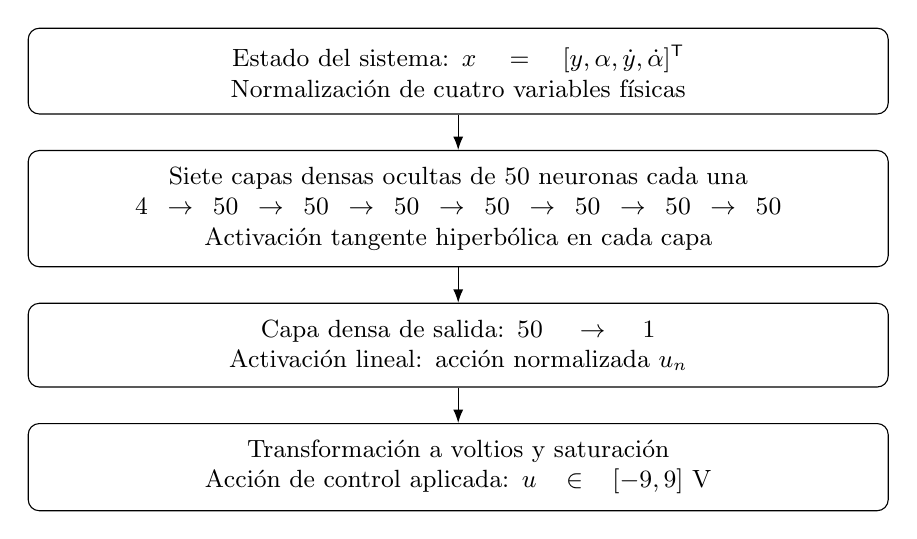
\begin{tikzpicture}[node distance=0.45cm, bloque/.style={draw,rounded corners,align=center,text width=10.5cm,inner sep=6pt,font=\small},>=Latex]
\node[bloque] (entrada) {Estado del sistema: $x=[y,\alpha,\dot y,\dot\alpha]^{\mathsf T}$\\Normalización de cuatro variables físicas};
\node[bloque,below=of entrada] (ocultas) {Siete capas densas ocultas de 50 neuronas cada una\\$4\rightarrow50\rightarrow50\rightarrow50\rightarrow50\rightarrow50\rightarrow50\rightarrow50$\\Activación tangente hiperbólica en cada capa};
\node[bloque,below=of ocultas] (salida) {Capa densa de salida: $50\rightarrow1$\\Activación lineal: acción normalizada $u_n$};
\node[bloque,below=of salida] (accion) {Transformación a voltios y saturación\\Acción de control aplicada: $u\in[-9,9]\ \mathrm{V}$};
\draw[->] (entrada) -- (ocultas);
\draw[->] (ocultas) -- (salida);
\draw[->] (salida) -- (accion);
\end{tikzpicture}
\caption{Arquitectura e interfaz de la red neuronal utilizada como aproximador del MPC. La normalización y la transformación de salida forman parte de la interfaz de inferencia.}
\label{fig:arquitectura_mpc_cap2}
\fuente{elaboración propia a partir del modelo utilizado en el caso de estudio}
\end{figure}

Si $h^{(0)}=x_n$ representa el estado normalizado, la evaluación de las capas puede escribirse como
\begin{align}
h^{(\ell)} &= \tanh\!\left(W^{(\ell)}h^{(\ell-1)}+b^{(\ell)}\right),\quad \ell=1,\ldots,7,\\
u_n &= W^{(8)}h^{(7)}+b^{(8)}.
\end{align}
Cada vector $h^{(\ell)}$ contiene 50 activaciones internas. La primera matriz de pesos combina las cuatro entradas; las seis siguientes combinan las 50 activaciones de la capa precedente. Finalmente, la matriz de salida reúne las últimas 50 activaciones en un escalar. La tangente hiperbólica introduce la no linealidad necesaria para representar una relación compleja entre estado y control. La salida lineal evita imponer en esa última capa el intervalo de una función sigmoide o de una tangente hiperbólica; el límite físico se aplica posteriormente, al recuperar la tensión del actuador.

La Tabla~\ref{tab:cap2_mlp} detalla las dimensiones y los parámetros de las ocho capas densas que componen la referencia utilizada en la memoria.

\begin{table}[H]\centering\small
\caption{Topología del controlador transferido a Keras.}\label{tab:cap2_mlp}
\begin{tabularx}{\linewidth}{Yrrr}\toprule
Capa & Entradas & Salidas & Parámetros\\\midrule
\texttt{dense\_0}, tanh & 4 & 50 & 250\\
\texttt{dense\_1}, tanh & 50 & 50 & 2550\\
\texttt{dense\_2}, tanh & 50 & 50 & 2550\\
\texttt{dense\_3}, tanh & 50 & 50 & 2550\\
\texttt{dense\_4}, tanh & 50 & 50 & 2550\\
\texttt{dense\_5}, tanh & 50 & 50 & 2550\\
\texttt{dense\_6}, tanh & 50 & 50 & 2550\\
\texttt{output\_u}, lineal & 50 & 1 & 51\\\midrule
Total & & & 15\,601\\\bottomrule
\end{tabularx}
\fuente{elaboración propia a partir de la arquitectura del controlador}
\end{table}
Los parámetros Float32 ocupan 62\,404 bytes, equivalentes a 60,94 KiB. El número de productos de las capas densas es $4\cdot50+6\cdot50^2+50=15\,250$, sin contabilizar activaciones, sesgos ni transformaciones de interfaz. Estos parámetros se mantienen fijos durante la evaluación de la referencia Float32.

\subsubsection{Transferencia de pesos y sesgos}
Equinox evalúa una capa con pesos almacenados como $(n_{\mathrm{out}},n_{\mathrm{in}})$, mientras que Keras almacena su matriz como $(n_{\mathrm{in}},n_{\mathrm{out}})$. Para conservar la transformación se asigna
\begin{equation}
W_{\mathrm{Keras}}=W_{\mathrm{EQX}}^{\mathsf T},\qquad b_{\mathrm{Keras}}=b_{\mathrm{EQX}}.
\end{equation}
Los pesos y sesgos se transfirieron directamente en representación Float32, conservando las activaciones de cada capa. La transposición de las matrices adapta su organización al convenio de Keras sin modificar los coeficientes de la transformación representada. Esta reconstrucción permite utilizar el modelo dentro del flujo de conversión y cuantización, manteniendo como referencia la política previamente aprendida.

La obtención de esta referencia no requirió un nuevo entrenamiento. En consecuencia, su caracterización se realiza mediante la comparación de salidas entre implementaciones y la evaluación del comportamiento en lazo cerrado. El ajuste posterior asociado al entrenamiento consciente de cuantización constituye una etapa distinta, cuyo propósito es adaptar los parámetros a una representación de menor precisión.

\subsubsection{Variables de entrada y normalización}
\label{sec:mpc_normalizacion}

La red neuronal utilizada como aproximador del controlador MPC recibe
el estado del sistema carro--péndulo, organizado según
\begin{equation}
    x =
    \begin{bmatrix}
        y & \alpha & \dot{y} & \dot{\alpha}
    \end{bmatrix}^{\mathsf T},
\end{equation}
donde $y$ es la posición del carro, expresada en metros;
$\alpha$ es el ángulo del péndulo, expresado en radianes;
y $\dot{y}$ y $\dot{\alpha}$ son sus respectivas velocidades
lineal y angular. Estas variables presentan diferentes unidades y
magnitudes, por lo que se transforman antes de ingresar a la red.

En esta memoria se replicó el procedimiento de normalización
implementado por los autores en el código complementario de su trabajo
sobre MPC aproximado adaptativo \cite{hose2024,hoserepo}.
El artículo describe la arquitectura y la implementación del
controlador, mientras que la definición explícita de esta
transformación se encuentra en el archivo
\texttt{neural\_network\_training/data/dataset.py} del repositorio.
En dicho archivo se calculan, para cada componente del estado, la
media de las muestras y el máximo de sus valores absolutos.

Considerando un conjunto de $N$ muestras, los parámetros de
normalización de la variable $j$ se definen como
\begin{equation}
    \mu_{x,j} = \frac{1}{N}\sum_{i=1}^{N}x_{i,j},
    \qquad
    s_{x,j} = \max_{1\leq i\leq N}|x_{i,j}|.
\end{equation}
La entrada normalizada se obtiene mediante
\begin{equation}
    x_{n,j} = \frac{x_j-\mu_{x,j}}{s_{x,j}},
    \qquad j=1,\ldots,4.
    \label{eq:normalizacion_estado_mpc}
\end{equation}

Esta operación centra cada variable respecto de su media y utiliza
como escala el máximo valor absoluto de los datos antes del centrado.
Por tanto, no corresponde a una estandarización mediante desviación
estándar ni a una transformación min--max. Asimismo, no impone
necesariamente un intervalo exacto de $[-1,1]$, debido al
desplazamiento introducido al restar la media.

Los coeficientes utilizados en la implementación de esta memoria,
presentados de forma redondeada y en el mismo orden que el vector
de estado, son
\begin{align}
    \mu_x &\approx
    \begin{bmatrix}
        0{,}000067 \\
        0{,}004411 \\
        0{,}000187 \\
        -0{,}003780
    \end{bmatrix},
    &
    s_x &\approx
    \begin{bmatrix}
        0{,}349999 \\
        6{,}283180 \\
        1{,}199999 \\
        9{,}999998
    \end{bmatrix}.
\end{align}
Cada componente de $\mu_x$ y $s_x$ tiene las unidades de la variable
física correspondiente, de modo que la entrada normalizada es
adimensional. Estos valores corresponden a los coeficientes
empleados en los ensayos de esta memoria; el procedimiento de
cálculo y aplicación se sustenta en el código de los autores,
sin atribuir estos valores numéricos al texto del artículo.

Para la acción de control se aplica el mismo criterio de
normalización durante la preparación de los datos. En la inferencia,
la red entrega una salida normalizada $u_n$, que se transforma
nuevamente a voltios mediante
\begin{equation}
    \widetilde{u} = s_u u_n + \mu_u,
    \qquad
    \mu_u \approx -0{,}007703\ \mathrm{V},
    \qquad
    s_u = 9\ \mathrm{V}.
    \label{eq:desnormalizacion_control_mpc}
\end{equation}
Posteriormente, la acción aplicada se limita al intervalo de
operación del actuador:
\begin{equation}
    u = \operatorname{sat}_{[-9\,\mathrm{V},\,9\,\mathrm{V}]}
        \left(\widetilde{u}\right).
\end{equation}
La saturación constituye una operación posterior a la
desnormalización. Esta secuencia reproduce la implementada en
la función \texttt{call\_control} del archivo
\texttt{neural\_network\_training/tester/run\_testing.py}
del repositorio de los autores \cite{hoserepo}.

Las implementaciones en Equinox y Keras utilizan el mismo orden
de entradas, los mismos coeficientes y las mismas transformaciones
de salida. De esta forma, la comparación de fidelidad numérica
se realiza bajo una interfaz común y permite evaluar las
diferencias entre ambas implementaciones sin introducir cambios
en el preprocesamiento de los estados ni en la recuperación
de la acción de control.


\subsubsection{Síntesis de las referencias utilizadas}
La referencia de radiografías es una CNN de 22\,700 parámetros guardada al finalizar la quinta época. La referencia MPC es una MLP de 15\,601 parámetros transferida desde Equinox sin nuevo entrenamiento, con siete capas ocultas de 50 neuronas y una salida lineal.

Las estrategias de la sección~\ref{cap:cuant} se evaluarán respecto de estas referencias, distinguiendo fidelidad numérica, desempeño funcional y ejecución en la placa. La validación de transferencia complementa el análisis en lazo cerrado del controlador.

\section{Estrategias de cuantización}
\label{sec:estrategias_experimentales}

Las variantes se obtuvieron a partir de los pesos de referencia de cada caso. Se consideraron Float32, PTQ INT8, QAT INT8, INT16x8 y precisión mixta selectiva, siguiendo las definiciones de la sección~\ref{cap:cuant}. En MPC se distinguieron además PTQ por tensor y por canal; en radiografías se evaluaron dos selecciones mixtas, con tres y cinco nodos preservados en precisión flotante. Las conversiones enteras utilizaron datos representativos ya sometidos al mismo procesamiento de entrada que el modelo de referencia~\cite{cap5_ptq}.

\begin{table}[htbp]
\centering
\caption{Configuraciones de calibración y ajuste empleadas.}
\label{tab:ajuste_cap5}
\begingroup\small\setstretch{1.05}
\begin{tabularx}{\textwidth}{@{}>{\raggedright\arraybackslash}p{2.8cm}YY@{}}
\toprule
Procedimiento & Radiografías & MPC \\
\midrule
Calibración PTQ y mixta & Primeras 350 imágenes de entrenamiento usadas por el generador. & 5000 estados normalizados, sin reemplazo, semilla 100. \\
Datos para QAT & 2279 imágenes de ajuste y 403 de validación. & 50000 pares estado--acción; 45000 de ajuste y 5000 de validación, semilla 123. \\
Optimización QAT & Adam, $10^{-5}$; entropía cruzada categórica dispersa; lote 32. & Adam, $10^{-5}$; error cuadrático medio; lote 256. \\
Finalización QAT & Máximo 15 épocas; parada temprana con paciencia 4. & Máximo 20 épocas; parada temprana con paciencia 4. \\
Selección de pesos & Restauración de los pesos de menor pérdida de validación. & Restauración de los pesos de menor pérdida de validación. \\
\bottomrule
\end{tabularx}
\endgroup
\end{table}

En QAT se ajustaron los pesos bajo la simulación de cuantización y posteriormente se exportó el modelo~\cite{cap5_qat}. En radiografías se añadió una reducción de la tasa de aprendizaje por un factor 0,5 tras dos épocas sin mejora, con mínimo $10^{-7}$. Los registros de entrenamiento documentan ocho épocas de ajuste en radiografías y siete en MPC; los máximos de la tabla son límites configurados, no el número de épocas efectivamente ejecutado. La calibración de la exportación QAT radiográfica utilizó 350 imágenes del subconjunto de ajuste, seleccionadas con semilla 42.

La precisión mixta se construyó a partir del diagnóstico de error por nodo. En radiografías se ordenó la raíz del error cuadrático medio (RMSE) dividida por la escala del cuantizador y se preservaron tres o cinco nodos según la variante. El criterio priorizaba errores superiores a 0,7, pero completaba la cantidad solicitada con el ranking restante. Por tanto, la selección ejecutada no equivale a conservar exclusivamente los nodos que superan ese umbral~\cite{cap5_debugger,cap5_registros}.

En MPC se conservaron en Float32 la primera capa y la salida, y se aplicó un umbral de 0,32 a las capas internas. La selección obtenida mantuvo también en Float32 las capas \texttt{dense\_2} a \texttt{dense\_5}, mientras que \texttt{dense\_1} y \texttt{dense\_6} permanecieron cuantizadas. El interés experimental de esta variante fue preservar las regiones sensibles y evaluar el compromiso resultante en el controlador completo.

La interfaz de entrada y salida se trató como una propiedad de cada archivo. INT16x8 conservó interfaces Float32; las variantes mixtas emplearon INT8 en radiografías y Float32 en MPC. Además, el generador radiográfico produjo una versión PTQ con interfaz INT8, mientras que la comparación posterior cargó otra versión PTQ con interfaz Float32. Cada resultado debe asociarse al archivo concreto evaluado, sin considerar ambas exportaciones intercambiables.

Las comprobaciones documentadas abarcan la inspección de tipos y parámetros de cuantización y, en las variantes mixtas, la revisión de la composición del grafo. Su alcance varía entre programas: existe una función de auditoría aplicada a variantes MPC y verificaciones específicas en radiografías. No se dispone de una auditoría exhaustiva de todas las conversiones. Para el despliegue se contrastó asimismo el modelo exportado con el informe del compilador, en relación con la sección~\ref{sec:cap4_compilacion}.

\section{Evaluación y validación}
\label{sec:evaluacion_validacion}

\subsection{Comprobación de la transferencia MPC}\label{sec:comparacion_transferencia}
\subsubsection{Comparación sobre entradas idénticas}
La fidelidad de la transferencia se evaluó sobre los primeros 10\,000 estados del conjunto de datos, aplicando la misma normalización y entregando entradas idénticas a ambas implementaciones. Este procedimiento permite medir las diferencias introducidas por la representación computacional de la red antes de estudiar su efecto sobre la evolución de la planta.

Para $e_i=u_i^{\mathrm{Keras}}-u_i^{\mathrm{EQX}}$ se calculan
\begin{align}
\mathrm{RMSE}&=\sqrt{\frac{1}{n}\sum_{i=1}^{n}e_i^2},\label{eq:rmse}\\
\mathrm{MAE}&=\frac{1}{n}\sum_{i=1}^{n}|e_i|,\qquad
E_{\max}=\max_i|e_i|.
\end{align}
Primero se comparan salidas normalizadas. Después se aplica la desnormalización y, en ambos modelos, una saturación a $[-9,9]$ V. El segundo grupo de métricas caracteriza, por tanto, la acción desnormalizada y saturada que se entrega al sistema.


Sin saturación, una transformación afín común multiplicaría cada error por $s_u$. La saturación puede reducir diferencias en los extremos; por ello, las métricas físicas se calculan directamente a partir de las acciones finales de ambas implementaciones.
\subsubsection{Contraste con la evaluación en lazo cerrado}
La evaluación de las dos implementaciones en lazo cerrado utilizó el banco común de 200 condiciones iniciales descrito en la sección~\ref{sec:mpc_transferencia}, con el procedimiento de simulación indicado a continuación.


Los resultados de estas comparaciones se presentan en la sección~\ref{sec:equivalencia_mpc}.

\subsection{Evaluación funcional en el computador}

En radiografías se compararon las predicciones sobre las mismas 624 imágenes mediante exactitud, precisión, sensibilidad, medida F1 y matriz de confusión. La clase se obtuvo a partir de la mayor puntuación de salida. Se calculó además el RMSE de las puntuaciones respecto de Float32 para distinguir la conservación de la decisión de clasificación de la conservación numérica de la salida.

La medición temporal en el computador utilizó el intérprete TensorFlow Lite con cuatro hilos y diez invocaciones de calentamiento. El intervalo cronometrado comprendió únicamente la llamada de inferencia, dejando fuera la preparación y copia de entradas. Se registraron media, mediana, desviación estándar y percentil 95. La comparación de tamaño se realizó entre archivos TensorFlow Lite, incluida la referencia Float32, para evitar que diferencias entre contenedores se interpretaran como reducción de memoria de la red.

En MPC se evaluaron primero las salidas para entradas comunes y luego el comportamiento en lazo cerrado. Se utilizó el banco de 200 condiciones iniciales descrito en la sección~\ref{sec:mpc_transferencia}. Cada simulación duró 16 s, con período de muestreo de 0,16 s y 100 acciones de control. La planta nominal se integró mediante \texttt{odeint}, manteniendo constante la acción durante cada intervalo.

El criterio principal de éxito exigió mantener $|y|<0{,}4$ m durante la trayectoria y alcanzar, en las últimas diez muestras, $|y|<0{,}1$ m y un error angular menor que 0,17 rad, junto con la limitación de voltaje. El evaluador de referencia aplica además cotas globales de 100 rad, 100 m/s y 100 rad/s al ángulo reducido y a las dos velocidades; en las últimas diez muestras, limita las velocidades a 100 m/s y 170 rad/s. Se conserva este predicado completo al contabilizar los éxitos. El ángulo se reduce al intervalo principal para evaluar el error angular, pero la simulación de referencia entrega al controlador el ángulo continuo. La tasa de éxito se calcula sobre las 200 condiciones de ese banco y no se atribuye a la placa.

\subsection{Compilación, validación estática e integración por UART}\label{sec:validacion_st}

Los archivos seleccionados se importaron a la cadena ST para analizar su compatibilidad, generar la implementación y validar las salidas con entradas conocidas~\cite{cap5_stcompiler,cap5_stvalidacion}. Se registraron el formato exportado, la representación admitida por el compilador, la asignación de operadores y los recursos informados. En particular, una ejecución con sustituciones de precisión o procesamiento software se identifica como tal al presentar sus resultados.

En radiografías, el proyecto de validación identifica la variante mixta de cinco nodos y utiliza AI Runner mediante el puerto serie a 115200 bit/s~\cite{cap5_integracion}. El computador carga las ocho imágenes del archivo de validación y adapta sus entradas a INT8, con forma $1\times150\times150\times1$, escala $0{,}00392156885936856$ y punto cero $-128$. Cada inferencia devuelve dos valores INT8, con escala $1/256$ y punto cero $-128$. Se comparan las salidas de la implementación en placa con las del archivo TensorFlow Lite de referencia, además de contrastarlas con las etiquetas disponibles.

El programa principal activa el servicio de validación de ST. Su middleware para Neural-ART recibe los tensores, ejecuta la red, recoge los contadores de tiempo y devuelve las salidas mediante Protocol Buffers. El proyecto conserva informes de análisis, generación y validación en destino, que vinculan el modelo con su configuración y sus resultados. Esta ruta utiliza el protocolo oficial de ST. La demostración de 16 imágenes emplea una aplicación distinta con mensajes \texttt{XRAY}/\texttt{RESULT}; compartir el puerto serie no acredita que ambas utilicen el mismo ejecutable.

\subsubsection{Alcance del análisis de los archivos compilados}\label{sec:analisis_listados}
Un archivo de listado o desensamblado permite inspeccionar las instrucciones y los símbolos incluidos en el ejecutable. En esta memoria se analizaron, entre otros, \texttt{PTQ\_\allowbreak MIX\_\allowbreak SELECTIVE\_\allowbreak CM55.list} y \texttt{PTQ\_\allowbreak MIX\_\allowbreak SELECTIVE\_\allowbreak NPU.list}. Los extractos de la sección~\ref{sec:cap4_evidencia} proceden de esos artefactos experimentales \cite{cap4_evidence}. Las direcciones identifican posiciones dentro de cada compilación y no constituyen direcciones universales para otras versiones del firmware.

La evidencia estática permite reconocer instrucciones y llamadas entre funciones. Una llamada identificada dentro de una ruta asociada a la red ofrece mayor información que encontrar un símbolo aislado en el binario. Sin embargo, el listado no registra cuántas veces se ejecutó cada instrucción durante una prueba ni su duración. Esas preguntas se resuelven con mediciones y perfiles de ejecución.


\subsection{Validación HIL de la alternativa MPC seleccionada}\label{sec:hil_seleccionada}
El banco utiliza un controlador físico y una planta simulada de paso fijo. Su sincronización con el tiempo de pared se evalúa por separado; la denominación HIL no implica aquí una garantía de ejecución estricta en tiempo real.


La comparación de estrategias de cuantización se desarrolla en el computador y mediante la validación de inferencia en placa. Como etapa de integración se seleccionó la alternativa de precisión mixta para el banco HIL. Esta etapa evalúa el controlador desplegado dentro del lazo de realimentación; no constituye una comparación HIL de todas las cuantizaciones. La configuración de ejecución, incluida su asignación a Cortex-M55 o NPU, se identifica con el proyecto compilado y sus informes, sin deducirla del formato Float32 de la interfaz.

El computador integra la planta y la STM32 calcula la acción de control. En cada instante se transmiten el identificador de muestra y los cuatro estados físicos, sin normalizar. El firmware normaliza la entrada, ejecuta la red, recupera la tensión y devuelve la acción, la salida normalizada, los ciclos de inferencia y el estado de ejecución. La solicitud ocupa 24 bytes y la respuesta 28. El programa comprueba cabecera, identificador y estado de ejecución antes de avanzar la planta. Esta comunicación utiliza el protocolo HIL personalizado y no el servicio de validación ST empleado en la etapa anterior.

La actualización del procedimiento establece una convención angular común con la simulación de referencia: se conserva el ángulo continuo en la transmisión y en la preparación de entrada del firmware. Para ello, se sustituye la reducción angular por el valor directo del estado tanto en el emisor Python como en el arreglo previo a la normalización en C. La reducción a $[-\pi,\pi)$ se mantiene exclusivamente para calcular y representar el error respecto del equilibrio. Así, la normalización se realiza una sola vez en el firmware. La versión anterior reducía el ángulo antes de la inferencia; sus registros se distinguen de los obtenidos con el procedimiento actualizado~\cite{cap5_hil_actualizado}.

La correspondencia entre código y ejecución forma parte de la identificación del ensayo.\footnote{Compilar o iniciar una sesión del cargador FSBL no demuestra que se haya actualizado la aplicación MPC. La confirmación requiere identificar el binario de aplicación cargado o inspeccionar la entrada efectiva de la red. El registro del ángulo continuo de la planta no acredita por sí solo el valor transmitido. Esta verificación se realiza fuera de las mediciones temporales si requiere detener el procesador.}

Para ampliar la evaluación más allá de una trayectoria, se definió el barrido de ocho condiciones de la tabla~\ref{tab:hil_ocho}. Se varía únicamente el ángulo inicial, manteniendo posición y velocidades iniciales nulas. Los pares de signos permiten observar respuestas desde ambos sentidos, mientras que las amplitudes pequeñas, intermedias y próximas a $\pi$ exploran distintos puntos de partida. La selección es determinista; no es una muestra aleatoria representativa de todo el dominio ni reemplaza las 200 condiciones de simulación.

\begin{table}[htbp]
\centering\small
\caption{Condiciones iniciales definidas para el barrido HIL de precisión mixta.}
\label{tab:hil_ocho}
\begin{tabular}{ccccc}
\toprule
Caso & $y_0$ [m] & $\alpha_0$ [rad] & $\dot y_0$ [m/s] & $\dot\alpha_0$ [rad/s] \\
\midrule
1 & 0 & $+0{,}10$ & 0 & 0 \\
2 & 0 & $-0{,}10$ & 0 & 0 \\
3 & 0 & $+0{,}30$ & 0 & 0 \\
4 & 0 & $-0{,}30$ & 0 & 0 \\
5 & 0 & $+1{,}00$ & 0 & 0 \\
6 & 0 & $-1{,}00$ & 0 & 0 \\
7 & 0 & $+3{,}13$ & 0 & 0 \\
8 & 0 & $-3{,}13$ & 0 & 0 \\
\bottomrule
\end{tabular}
\end{table}

Cada ensayo se configura con duración de 16 s, período de 0,16 s y 100 acciones. Se mantiene el mismo firmware, modelo, normalización e integrador \texttt{odeint}, con acción constante durante cada intervalo. Las solicitudes se atienden secuencialmente por UART a 115200 bit/s, sin breakpoints activos. Cada condición se registra en un CSV independiente con estados, acciones, tiempos y avisos de incumplimiento temporal. Se preservan los registros incompletos como incidencias de ejecución y no se clasifican automáticamente como fallos de estabilización. El capítulo de resultados presenta los ensayos y los registros que sustentan su evaluación.

La evaluación HIL comprueba $|y|<0{,}4$ m durante la trayectoria muestreada, $|y|<0{,}1$ m y $|e_\alpha|<0{,}17$ rad en las últimas diez muestras, y la tensión dentro de $[-9,9]$ V. Estas comprobaciones no reproducen las cotas amplias de velocidad del evaluador original. Por tanto, se informa el cumplimiento de los criterios HIL sobre las condiciones efectivamente completadas; solo se compara con una tasa de simulación cuando coinciden las condiciones iniciales y el predicado de evaluación.

Se distingue también el instante registrado: el programa guarda el estado previo a cada acción, por lo que el CSV de 100 filas abarca de 0 a 15,84 s. Para evaluar el horizonte completo se reconstruye el estado de 16 s con el integrador de la planta, el último estado registrado y la última acción. La trayectoria analizada contiene así 101 estados y su ventana terminal de diez muestras corresponde a 14,56--16,00 s. El estado final es calculado, no una medición adicional contenida en el CSV. La reproducción de los pasos anteriores permite comprobar la consistencia de la reconstrucción con el registro. Esta es la ventana utilizada en los resultados HIL; las diez últimas filas del CSV, por sí solas, abarcarían una ventana diferente. El cumplimiento al final del horizonte describe ese ensayo y no demuestra estabilidad para tiempos arbitrariamente largos.

\subsection{Medición temporal, memoria y alcance de los resultados}

En el firmware MPC, el contador de ciclos DWT delimita la llamada de ejecución de la red. La conversión a microsegundos se calibra frente al contador de milisegundos del sistema durante una ventana de 10 ms; la frecuencia declarada del núcleo se usa como alternativa si esa calibración no resulta válida. La normalización, la transformación de salida y la comunicación quedan fuera de ese intervalo. Por separado, el computador mide el tiempo de ida y vuelta de la solicitud UART, que incluye transferencia, atención de la petición y recepción de la respuesta.

El programa HIL registra media, percentil 99 y máximo de ambos tiempos. Compara cada tiempo de ida y vuelta con el período de 0,16 s y contabiliza por separado los ciclos tardíos del computador, cuyo trabajo incluye integración y representación gráfica. De forma predeterminada intenta acompasar las iteraciones al tiempo de pared mediante esperas; la opción de ejecución sin sincronización elimina esas esperas. Este mecanismo permite observar incumplimientos temporales, pero no constituye una garantía de tiempo real estricto.

En radiografías se mantiene la misma distinción entre transferencia e inferencia. En la aplicación con entrada INT8, la carga útil de una imagen contiene 22500 bytes, sin incluir cabeceras ni respuestas. Su transferencia a 115200 bit/s forma parte del tiempo de aplicación y no del costo computacional de la CNN. Otras interfaces requieren calcular el volumen según el tipo de datos efectivamente transmitido. En el proyecto de validación, el middleware recibe la entrada antes de ejecutar la red y devuelve después los contadores recogidos durante su ejecución. El informe separa el procesamiento hardware, el software y el control de ejecución. Esta latencia se distingue del tiempo total de transferencia por UART.

La memoria se analizó diferenciando tamaño del modelo exportado, almacenamiento de parámetros y búferes de activaciones. Las dos últimas magnitudes dependen de la implementación compilada y de su configuración de memoria; no se deducen únicamente del tamaño del archivo TensorFlow Lite. No se dispone de una caracterización homogénea de la ocupación total Flash y RAM del firmware para todas las variantes. Los fallos de enlace o asignación documentan restricciones de configuraciones concretas, pero no sustituyen esa medición global. De igual modo, los listados de ensamblado se utilizaron como evidencia de instrucciones y rutas presentes, con el alcance estático de la sección~\ref{sec:analisis_listados}.

La selección final se realiza dentro de cada tarea, considerando desempeño funcional, latencia y memoria de la implementación ejecutada. Cada resultado se vincula con su conjunto de evaluación y nivel de ejecución. Las métricas de clasificación y control se presentan por separado. El tamaño, los ciclos y el esfuerzo de control no se consideran mediciones de energía eléctrica.


\section{Validación complementaria en NUCLEO-L476RG}\label{sec:metodo_l476}
La campaña complementaria utiliza ST Edge AI Core 4.0.1 para validar los modelos exportados en una NUCLEO-L476RG. Se conservaron los registros de generación, compilación, validación y los listados de instrucciones. El clasificador QAT se evaluó sobre ocho imágenes y cinco variantes MPC sobre 200 entradas por modelo. Las comparaciones se emparejaron mediante el hash del modelo informado por ST y el conjunto de entrada identificado en los comandos; los intentos fallidos se registraron separadamente sin asignarles métricas de inferencia.

Se extrajeron latencia, ciclos de CPU, error cruzado, pesos y activaciones. Para la memoria se utilizó el primer resumen de generación, evitando mezclarlo con la representación de referencia que puede aparecer después en la validación NPU. Los perfiles identifican CPU a 80 MHz en L476 y a 800 MHz en N657. Los registros de la campaña complementaria identifican rutas de STM32CubeIDE 2.2.0 y herramientas GNU 14.3.1; las bibliotecas CPU precompiladas se identifican como runtime 12.0.1, compilado con GCC 13.3.1. Estas versiones se conservan como metadatos de la campaña complementaria, sin asumir que todos los objetos se recompilaron con las mismas opciones.

La revisión estática incluye los seis listados L476 y los dos QAT radiográficos N657. Se distinguieron registros Q y predicación MVE, aritmética escalar y operaciones DSP empaquetadas del M4. La comparación entre placas no se diseñó como una prueba con Helium activado y desactivado en el mismo procesador; por ello se examinaron conjuntamente frecuencias, ciclos, instrucciones y latencia. No se realizaron nuevos ensayos HIL en L476 dentro de esta campaña.


\chapter{Resultados}\label{cap:resultados}
\FloatBarrier
\section{Organización y alcance de la evidencia}
Este capítulo presenta los resultados del clasificador de radiografías y del controlador neuronal que aproxima la política MPC. La exposición sigue la secuencia experimental del capítulo anterior: evaluación en computador, conversión y compilación, validación numérica en la STM32N6570-DK y pruebas de integración. Se incorpora una comparación complementaria con NUCLEO-L476RG, que cierra el capítulo. Para radiografías, se estudian la clasificación y el costo de inferencia; para MPC, se añade el comportamiento de la planta simulada en lazo cerrado. La comparación permite examinar qué parte del beneficio de cuantizar el modelo se conserva después de implementarlo.

La evidencia experimental comprende predicciones, matrices de confusión, registros de ST Edge AI, grafos de los modelos, listados de instrucciones y ocho ensayos HIL \cite{res_archivo2026}. La campaña complementaria comprende validaciones QAT del clasificador en STM32N6 y registros de NUCLEO-L476RG para ambos casos de estudio \cite{res_ampliacion2026}. Las tablas y figuras sintetizan las mediciones y los cálculos derivados de estos registros. En el análisis se distingue entre resultados medidos, magnitudes calculadas e interpretación de los hallazgos.

\begin{table}[htbp]\centering\small
\caption{Conjuntos de evidencia utilizados y alcance de cada comparación.}\label{tab:res_alcance}
\begin{tabularx}{\linewidth}{p{3.5cm}p{2.6cm}Y}\toprule
Evaluación & Muestras & Resultado que permite examinar\\\midrule
Radiografías en PC & 624 imágenes & Clasificación, concordancia y recursos del archivo\\
Radiografías con ST & 8 imágenes & Fidelidad de la implementación y perfil de inferencia\\
Demostración UART & 16 imágenes & Recepción, ejecución y respuesta de la aplicación\\
MPC en simulación & 200 estados iniciales & Cumplimiento del criterio de lazo cerrado\\
MPC con ST & 200 entradas & Concordancia numérica por inferencia y perfil\\
MPC en HIL & 8 ensayos; 100 acciones cada uno & Trayectorias, restricciones y tiempos UART/inferencia\\\bottomrule
\end{tabularx}
\fuente{registros experimentales}
\end{table}

Los conjuntos de ocho, dieciséis y 624 radiografías se interpretan por separado. De igual forma, las 200 entradas utilizadas en la validación ST no son las 200 condiciones iniciales de las simulaciones: la primera prueba compara salidas para entradas aisladas; la segunda evalúa trayectorias de 16 s. Las ocho condiciones HIL constituyen una selección determinista y no una repetición de toda la campaña de simulación.

El tamaño del archivo exportado, los pesos compilados y el búfer de activaciones se presentan como magnitudes diferentes. Las cifras de memoria de red no incluyen necesariamente todo el programa, la pila, el transporte UART o los datos de la aplicación. Tampoco se convierten los tiempos en consumo energético, puesto que los archivos no contienen mediciones eléctricas de estas ejecuciones.

\begin{table}[htbp]\centering\small
\caption{Cobertura de evaluación por variante y destino.}\label{tab:cobertura_variantes}
\begin{tabularx}{\linewidth}{Ycccc}\toprule
Caso y variante & PC & N6 CPU & \shortstack{Ruta N6\\Neural-ART} & L476\\\midrule
Radiografías Float32 & Sí & ND & ND & ND\\
Radiografías PTQ INT8 & Sí & Sí & Sí & Fallo\\
Radiografías QAT INT8 & Sí & Sí & Sí & Sí\\
Radiografías INT16x8 & Sí & Sí & Sí$^{*}$ & ND\\
Radiografías Mixed-3 & Sí & ND & ND & ND\\
Radiografías Mixed-5 & Sí & Sí & Sí & Fallo\\\midrule
MPC Float32 & Sí & Sí & ND & ND\\
MPC PTQ INT8 por tensor & Sí & Sí & Sí & Sí\\
MPC PTQ INT8 por canal & Sí & Sí & Sí & Sí\\
MPC QAT INT8 & Sí & Sí & Sí & Sí\\
MPC INT16x8 & Sí & Sí & ND & Sí\\
MPC precisión mixta & Sí & Sí & Sí & Sí\\\bottomrule
\end{tabularx}
\fuente{evaluaciones en PC y registros de validación ST de la campaña}
\par\smallskip\footnotesize El asterisco señala una ruta INT16x8 cuya ejecución nativa no está acreditada y que presenta discrepancias de salida. Sí indica una evaluación completada; en placa incluye generación y validación, sin certificar auditoría integral ni ejecución nativa de todos los operadores. N6 NPU identifica la ruta configurada con Neural-ART, que puede incluir software. ND significa que no se dispone de una validación independiente. Fallo identifica un intento sin validación completada. El HIL se limita a MPC mixto; la demostración radiográfica UART corresponde a Mixed-5.
\end{table}

\FloatBarrier
\section{Clasificación de radiografías: evaluación en computador}
\FloatBarrier
\subsection{Evolución del entrenamiento y ajuste con cuantización}
La Tabla~\ref{tab:cap2_epocas} y la Figura~\ref{fig:cap2_curvas} presentan los valores registrados de pérdida y exactitud durante las cinco épocas. La pérdida expresa el criterio numérico utilizado para ajustar los parámetros, mientras que la exactitud describe el resultado de clasificación. Su evolución conjunta permite contrastar el ajuste y la validación.

\begin{table}[H]\centering\small
\caption{Pérdida y exactitud registradas durante el entrenamiento de la CNN.}\label{tab:cap2_epocas}
\begin{tabular}{rrrrr}\toprule
Época & Pérdida train & Exactitud train & Pérdida val & Exactitud val\\\midrule
1 & 0,5278 & 0,7617 & 0,4278 & 0,7901\\
2 & 0,2488 & 0,8941 & 0,3639 & 0,8365\\
3 & 0,1800 & 0,9284 & 0,3950 & 0,8253\\
4 & 0,1484 & 0,9452 & 0,6838 & 0,7628\\
5 & 0,1469 & 0,9433 & 0,5848 & 0,7981\\\bottomrule
\end{tabular}
\fuente{registros del entrenamiento de la CNN; exactitud expresada como fracción}
\end{table}

\begin{figure}[H]\centering
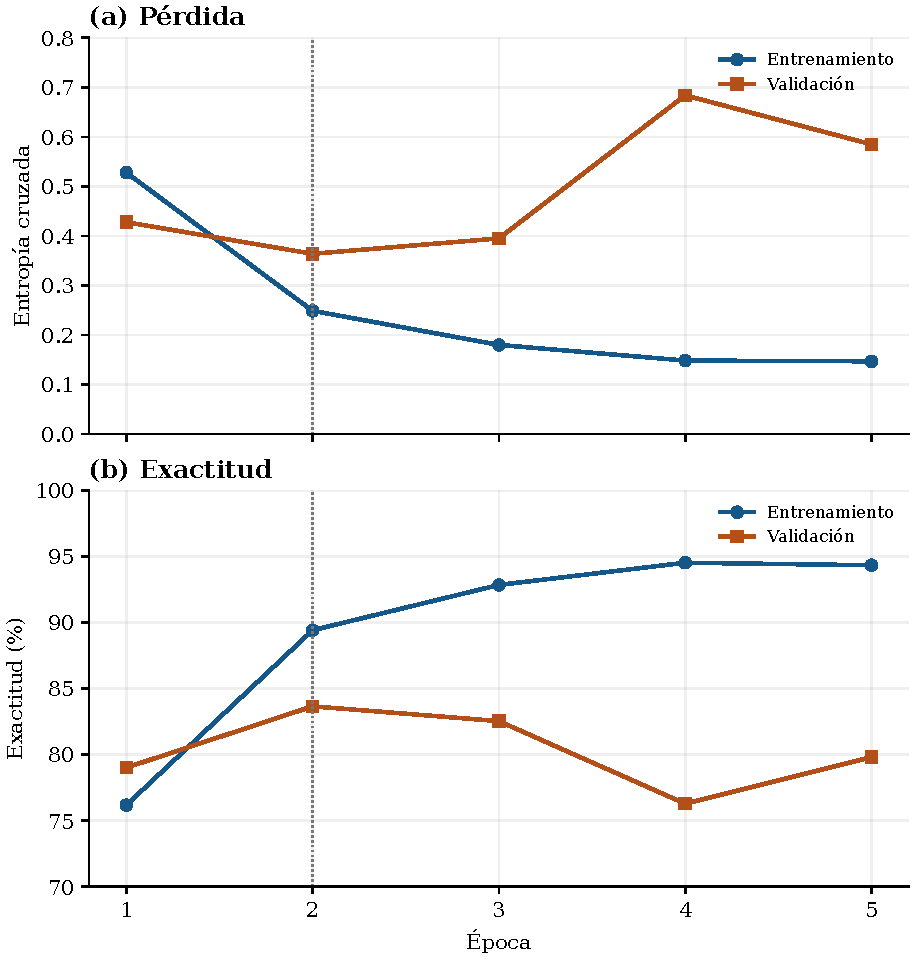
\includegraphics[width=.81\linewidth]{figuras/cap2_curvas_cnn.pdf}
\caption{Evolución de la pérdida y la exactitud registradas durante el entrenamiento de la CNN. La línea vertical identifica la época 2, de menor pérdida y mayor exactitud de validación entre las cinco épocas registradas.}\label{fig:cap2_curvas}
\fuente{elaboración propia a partir de los registros de entrenamiento}
\end{figure}

La menor pérdida de validación, 0,3639, y la mayor exactitud de validación, 83,65\%, se alcanzaron en la segunda época. Al finalizar la quinta época, la pérdida de validación fue 0,5848 y la exactitud, 79,81\%. Por consiguiente, el modelo seleccionado como referencia corresponde al estado final del entrenamiento, cuyo desempeño se distingue del mejor valor intermedio observado.

La reducción de la pérdida de entrenamiento acompañada por el deterioro de la validación a partir de la segunda época es compatible con sobreajuste. Este fenómeno ocurre cuando el modelo se adapta a particularidades de las muestras de entrenamiento que no se traducen en una mejora sobre otras muestras. En la quinta época, los valores registrados de exactitud de entrenamiento y validación presentan una diferencia de 14,52 puntos porcentuales. Este comportamiento motiva evaluar las variantes cuantizadas con un protocolo común, de modo que sus diferencias se interpreten respecto de la misma referencia.

El conjunto de evaluación se utilizó también para supervisar la validación durante el entrenamiento, sin intervenir en el cálculo de los gradientes. En consecuencia, los resultados caracterizan el desempeño sobre el conjunto empleado en el desarrollo y permiten comparar las variantes en condiciones compartidas; su alcance no corresponde a una validación externa independiente.
La campaña QAT posterior registra ocho épocas efectivamente ejecutadas, aunque se había establecido un máximo de quince. El programa informa detención anticipada y restauración de los pesos de la época 4, cuya pérdida de validación interna fue 0,102449. Para este ajuste se utilizaron 2279 imágenes de entrenamiento y 403 de validación interna; la comparación final conserva las 624 imágenes del conjunto de evaluación. Por ello, la exactitud interna de QAT, próxima al 95\%, no se compara directamente con el 79,97\% obtenido sobre el conjunto final.

\resfig{rx_qat.pdf}{Pérdida y exactitud durante las ocho épocas QAT registradas. La línea vertical identifica los pesos restaurados por el procedimiento de detención anticipada.}{fig:res_rx_qat}{\texttt{historial\_\allowbreak qat.csv}}{.96}

La restauración de la mejor época modifica el punto del entrenamiento que se exporta. En consecuencia, las diferencias entre QAT y Float32 incluyen tanto la cuantización como el reajuste de los parámetros. No pueden atribuirse exclusivamente al redondeo de una misma red congelada.

\FloatBarrier
\subsection{Comparación de clasificación y errores por clase}
La evaluación comprende 234 imágenes NORMAL y 390 PNEUMONIA. Las métricas de la Tabla~\ref{tab:xrayres} se verificaron con las etiquetas y predicciones almacenadas para cada variante. Se considera PNEUMONIA como clase positiva. La exactitud balanceada permite observar conjuntamente la sensibilidad y la especificidad, evitando que el mayor número de imágenes de neumonía oculte el comportamiento sobre la clase NORMAL.
\begin{table}[H]
\centering\small
\caption{Desempeño de clasificación sobre 624 radiografías. Valores en porcentaje.}\label{tab:xrayres}
\begin{tabularx}{\linewidth}{Yrrrrr}\toprule
Variante & Exact. & Balanceada & Sensib. & Especif. & $F_1$\\\midrule
Float32 & 79,81 & 73,68 & 98,21 & 49,15 & 85,87\\
PTQ INT8 & 80,93 & 75,34 & 97,69 & 52,99 & 86,49\\
INT16x8 & 79,17 & 72,82 & 98,21 & 47,44 & 85,49\\
Mixed-3 & 79,49 & 73,25 & 98,21 & 48,29 & 85,68\\
Mixed-5 & 79,81 & 73,68 & 98,21 & 49,15 & 85,87\\
QAT INT8 & 79,97 & 74,06 & 97,69 & 50,43 & 85,91\\
\bottomrule\end{tabularx}
\fuente{\texttt{comparacion\_final\_modelos.csv}; comprobación con las predicciones almacenadas}
\end{table}

\resfig{rx_metricas.pdf}{Comparación de exactitud y especificidad en las seis variantes del clasificador.}{fig:res_rx_metricas}{elaboración propia a partir de las métricas verificadas}{1}

PTQ INT8 obtiene 505 clasificaciones correctas de 624, frente a 498 de Float32: la diferencia es de siete imágenes y 1,12 puntos porcentuales. Sin embargo, la sensibilidad se reduce de 98,21\% a 97,69\%, mientras que la especificidad aumenta de 49,15\% a 52,99\%. La mejora de exactitud observada está asociada principalmente a nueve imágenes NORMAL adicionales correctamente clasificadas, a costa de dos neumonías adicionales clasificadas como normales. Este intercambio queda explícito en las matrices de confusión.

\resfig{rx_confusiones.pdf}{Matrices de confusión de los modelos sobre 624 imágenes. Se muestran conteos y porcentajes por fila; las filas representan la clase real.}{fig:res_rx_confusiones}{predicciones y matrices CSV de la evaluación final}{1}

En todas las variantes se observa sensibilidad alta y especificidad considerablemente menor. Por ejemplo, Float32 clasifica correctamente 383 de las 390 neumonías, pero sólo 115 de las 234 imágenes normales. Por tanto, una exactitud cercana al 80\% no describe por sí sola un comportamiento equilibrado entre clases. Estos resultados caracterizan el conjunto utilizado en el desarrollo y no constituyen una validación clínica o externa.

La variante Mixed-5 reproduce las 624 decisiones de Float32. INT16x8 modifica cuatro decisiones y Mixed-3 modifica dos; en ambos casos las modificaciones corresponden a nuevas clasificaciones incorrectas respecto de la referencia. QAT cambia 17 decisiones, corrige nueve errores e introduce ocho, por lo que su mejora neta es de una imagen. La Tabla~\ref{tab:rx_pareadas} muestra el contraste emparejado y evita interpretar dos exactitudes iguales como prueba suficiente de identidad de las predicciones.
\begin{table}[H]
\centering\small
\caption{Cambios de decisión respecto de Float32 sobre las mismas imágenes.}\label{tab:rx_pareadas}
\begin{tabularx}{\linewidth}{Yrrr}\toprule
Variante & Corrige & Introduce error & Decisiones distintas\\\midrule
PTQ INT8 & 25 & 18 & 43\\
INT16x8 & 0 & 4 & 4\\
Mixed-3 & 0 & 2 & 2\\
Mixed-5 & 0 & 0 & 0\\
QAT INT8 & 9 & 8 & 17\\
\bottomrule\end{tabularx}
\fuente{cálculo propio a partir de \texttt{predicciones\_*.npz}}
\end{table}


Aunque PTQ INT8 alcanza la mayor exactitud observada, los resultados de una sola partición y de un único entrenamiento no demuestran que su ventaja sea sistemática. Mixed-5 ofrece una evidencia diferente: conserva las decisiones de la referencia en este conjunto y disminuye el tamaño del archivo. La comparación distingue el desempeño respecto de las etiquetas de la concordancia con Float32.

\FloatBarrier
\subsection{Tamaño, latencia en computador y diferencias de salida}
\begin{table}[H]
\centering\small
\caption{Tamaño y latencia de los modelos evaluados en el computador.}\label{tab:rx_recursos}
\begin{tabularx}{\linewidth}{Yrrrrr}\toprule
Variante & Archivo (B) & Red. (\%) & Media (ms) & P95 (ms) & RMSE salida\\\midrule
Float32 & 95\,652 & 0,00 & 0,173 & 0,276 & 0,000000\\
PTQ INT8 & 38\,824 & 59,41 & 0,531 & 0,913 & 0,519218\\
INT16x8 & 31\,672 & 66,89 & 9,258 & 12,128 & 0,007808\\
Mixed-3 & 31\,968 & 66,58 & 0,299 & 0,408 & 0,005246\\
Mixed-5 & 34\,128 & 64,32 & 0,251 & 0,389 & 0,003778\\
QAT INT8 & 29\,784 & 68,86 & 0,373 & 0,466 & 0,028257\\
\bottomrule\end{tabularx}
\fuente{\texttt{comparacion\_final\_modelos.csv}; reducción respecto de 95\,652 B}
\end{table}

\resfig{rx_recursos_host.pdf}{Tamaño TFLite y latencia media en el computador. La escala temporal es logarítmica para visualizar la diferencia de INT16x8.}{fig:res_rx_host}{\texttt{comparacion\_\allowbreak final\_\allowbreak modelos.csv}}{1}

La referencia utilizada en esta comparación es el archivo Float32 TFLite de 95\,652 B. Con esa base, PTQ INT8 reduce el tamaño en 59,41\%, Mixed-5 en 64,32\% y QAT INT8 en 68,86\%. La comparación utiliza archivos TFLite, de modo que las reducciones se calculan sobre un mismo formato de representación. El menor archivo registrado es QAT INT8, de 29\,784 B.

En el computador, Float32 registra la menor latencia media, 0,173 ms. INT16x8 requiere 9,258 ms, aproximadamente 53,57 veces ese tiempo, mientras que Mixed-5 requiere 0,251 ms. La reducción del número de bits no implica una reducción de latencia en todos los entornos: aquí se observan los tiempos del intérprete y de sus rutas de ejecución en el PC. Estos valores se mantienen separados de los tiempos medidos en la STM32.

El RMSE de las salidas respecto de Float32 es 0,003778 para Mixed-5 y 0,005246 para Mixed-3. PTQ INT8 presenta un RMSE mucho mayor, 0,519218, aun cuando su exactitud de clasificación es ligeramente superior. La comprobación con las matrices de salidas almacenadas reproduce ese valor. Una salida numéricamente diferente puede conservar el orden entre clases y, con ello, la decisión final. Por tanto, el RMSE de las dos salidas y la exactitud responden a preguntas distintas; tampoco debe interpretarse automáticamente cada salida como una probabilidad calibrada.

Existe además una diferencia de topología relevante para la interpretación. Los grafos y registros ST identifican 30\,682 parámetros en PTQ INT8, frente a 22\,700 en INT16x8 y la variante mixta. En el grafo PTQ se observan convoluciones con ocho canales, mientras que la referencia de entrenamiento utiliza seis. Esta evidencia impide tratar toda diferencia entre las variantes desplegadas como efecto aislado de la precisión. Además, las exportaciones PTQ con interfaz Float32 e INT8 se consideran artefactos distintos. Sin una correspondencia explícita de identificadores, topología e interfaz, no se atribuye al archivo desplegado la exactitud obtenida por otro archivo evaluado en PC. Los registros permiten comparar las implementaciones evaluadas, pero no demuestran que todos procedan de una única topología y de los mismos pesos antes de cuantizar.

\FloatBarrier
\section{Clasificación de radiografías: implementación en placa}
\FloatBarrier
\subsection{Fidelidad numérica y tiempo de inferencia}
Los registros de ST Edge AI Core 4.0.1 contienen una validación sobre ocho imágenes, cuatro por clase. El RMSE cruzado de la Tabla~\ref{tab:rx_placa} compara la salida de la implementación ejecutada con la salida del modelo de referencia importado. Un cero informado se limita a las entradas ensayadas y a la resolución del reporte; no acredita identidad matemática para entradas arbitrarias. La exactitud de la última columna compara, en cambio, la clase predicha por la placa con las etiquetas. Las métricas describen, por tanto, propiedades distintas.
\begin{table}[H]
\centering\small
\caption{Validación de radiografías sobre ocho entradas en la STM32N6570-DK.}\label{tab:rx_placa}
\begin{tabularx}{\linewidth}{Yrrrr}\toprule
Variante / ruta & Media (ms) & Mín.--máx. (ms) & RMSE cruzado & Exact. (\%)\\\midrule
INT8 / M55 & 16,621 & 16,580--16,659 & 0 & 75,0\\
INT8 / Neural-ART & 0,514 & 0,506--0,536 & $2,584\times10^{-3}$ & 75,0\\
INT16x8 / M55 & 53,240 & 52,966--53,325 & $3,871\times10^{-5}$ & 62,5\\
INT16x8 / Neural-ART & 0,600 & 0,591--0,627 & $3,171\times10^{-1}$ & 62,5\\
Mixta-5 / M55 & 52,481 & 52,434--52,594 & 0 & 75,0\\
Mixta-5 / Neural-ART & 104,700 & 103,735--104,928 & 0 & 75,0\\
QAT / M55 & 14,814 & 14,805--14,840 & 0 & 75,0\\
QAT / Neural-ART & 0,290 & 0,288--0,305 & $1,092\times10^{-2}$ & 62,5\\
\bottomrule\end{tabularx}
\fuente{registros de validación ST incluidos en el paquete experimental}
\end{table}

\resfig{rx_latencia_placa.pdf}{Latencia media en la STM32N6570-DK para las rutas Cortex-M55 y Neural-ART. La comparación temporal debe leerse junto con la fidelidad numérica de la Tabla~\ref{tab:rx_placa}.}{fig:res_rx_target}{perfiles ST sobre ocho entradas por implementación}{1}

PTQ INT8 registra 16,621 ms en Cortex-M55 y 0,514 ms por la ruta Neural-ART, equivalente a una razón de tiempos de 32,34. La exactitud del pequeño lote es 75\% en ambas rutas; el RMSE cruzado es cero en M55 y 0,002584 en Neural-ART. El resultado documenta una reducción importante de tiempo para esa implementación INT8, con una discrepancia numérica pequeña pero no nula en el acelerador. La exactitud de 75\% corresponde sólo a seis aciertos en ocho entradas y no sustituye a la evaluación de 624 imágenes.

El validador informa RMSE cruzado igual a cero para Mixed-5 en las dos rutas, sobre las entradas ensayadas. Sin embargo, la ruta Neural-ART necesita 104,700 ms, frente a 52,481 ms de Cortex-M55: resulta aproximadamente dos veces más lenta. Por tanto, conservar las salidas del modelo no garantiza aprovechar favorablemente la NPU. La ubicación de las operaciones Float32 y la fragmentación de la ejecución se examinan con el perfil por épocas.

El resultado INT16x8 requiere una interpretación particular. En M55, el reporte de generación indica formato flotante, 90\,800 B de pesos y 533\,652 B de activaciones; el tiempo medido es 53,240 ms. En la ruta Neural-ART, el perfil sí registra actividad hardware y un tiempo de 0,600 ms, pero el RMSE cruzado aumenta a 0,317093. Las salidas de referencia abarcan aproximadamente 0,0146--0,6532, mientras que las de la placa se concentran entre 0,4964 y 0,5049.

Aunque ambas implementaciones de referencia y destino obtienen 62,5\% de exactitud en ese lote Neural-ART, sus matrices de confusión son diferentes: la referencia presenta $(TN,FP,FN,TP)=(1,3,0,4)$ y la placa $(4,0,3,1)$. La igualdad de cinco aciertos sobre ocho imágenes oculta, por tanto, diferencias relevantes en las decisiones. El tiempo de 0,600 ms no se presenta como aceleración equivalente de INT16x8 nativo. La documentación delimita el soporte hardware a operadores y esquemas cuantizados compatibles \cite{cap4_stoperators}; el nombre del archivo de entrada no certifica la precisión realmente ejecutada.


La validación QAT utiliza el mismo hash de modelo en M55 y Neural-ART. M55 registra 14,814 ms, RMSE cruzado informado como cero y seis aciertos sobre ocho imágenes. Neural-ART registra 0,290 ms, RMSE cruzado 0,010918301 y cinco aciertos. Las matrices son $(TN,FP,FN,TP)=(2,2,0,4)$ en referencia/M55 y $(1,3,0,4)$ en NPU: aparece un falso positivo adicional. El cambio de 12,5 puntos porcentuales corresponde a un caso en un lote pequeño, no a una estimación sobre las 624 imágenes de la evaluación en computador.
\resfig{rx_qat_validacion_confusion.pdf}{Validación QAT del clasificador: concordancia de las rutas CPU y diferencia de decisión de la ruta Neural-ART en el lote de ocho imágenes.}{fig:qat_validacion}{matrices de confusión de los registros ST; la comparación incluye la validación L476 descrita al cierre del capítulo}{1}
El perfil QAT de Neural-ART asigna 98,9\% a hardware, 0\% a operadores software y 1,1\% a control software. Es la menor latencia radiográfica registrada, 43,6\% inferior a los 0,514 ms de PTQ INT8, pero no conserva todas las decisiones de referencia del lote. La razón de tiempos entre sus rutas M55 y NPU es 51,08; se trata de una comparación entre implementaciones, no de una medida aislada de una instrucción o unidad.

\FloatBarrier
\subsection{Memoria y transformación de los grafos}
\begin{table}[H]
\centering\small
\caption{Memoria de red informada durante la generación para radiografías.}\label{tab:rx_memoria}
\begin{tabularx}{\linewidth}{Yrr}\toprule
Variante / ruta & Pesos (B) & Activaciones (B)\\\midrule
INT8 / M55 & 30\,832 & 92\,496\\
INT8 / Neural-ART & 30\,689 & 112\,500\\
INT16x8 / M55 & 90\,800 & 533\,652\\
INT16x8 / Neural-ART & 22\,753 & 180\,000\\
Mixta-5 / M55 & 26\,000 & 533\,652\\
Mixta-5 / Neural-ART & 26\,289 & 781\,536\\
QAT / M55 & 22\,828 & 35\,704\\
QAT / Neural-ART & 22\,704 & 55\,368\\
\bottomrule\end{tabularx}
\fuente{primer resumen de \texttt{generate}; incluye búferes de entrada/salida en activaciones}
\end{table}

\resfig{rx_memoria_npu.pdf}{Distribución de memoria de red de todas las variantes radiográficas evaluadas en Neural-ART, incluido QAT.}{fig:rx_memoria_npu}{pesos RO y activaciones RW del primer resumen de generación; 1 KiB = 1024 B}{1}
Las categorías se representan por separado porque los pesos y el espacio de trabajo no equivalen a una única reserva de SRAM. No se incluyen aquí el código, la pila, el heap ni los búferes externos de la aplicación. La figura muestra volumen por categoría, no ubicación física en cada banco. Para QAT/NPU se usan 22\,704 B de pesos y 55\,368 B de activaciones de la generación; los 22\,840 B y 35\,720 B del resumen posterior de validación son diferentes y no se consideran intercambiables sin verificar el alcance de cada campo. Se mantienen las cifras del resumen de generación como base uniforme de esta comparación.
Las cifras de la Tabla~\ref{tab:rx_memoria} se toman del resumen de generación de cada implementación. Esto es especialmente importante en la ruta Neural-ART, porque los resúmenes posteriores pueden informar otros tamaños; la atribución exacta de cada campo a la implementación o a la referencia debe verificarse antes de combinarlos. Para Mixed-5, la generación asigna 781\,536 B a activaciones, mientras que el resumen de validación informa 533\,448 B; utilizar indistintamente ambos valores produciría una comparación inconsistente. El primero concuerda con la distribución de memoria detallada de la implementación generada.

En Mixed-5, la ruta Neural-ART incrementa el búfer de activaciones en 46,45\% respecto de M55. En INT8, el incremento es de 21,63\%. Los pesos de la red y el búfer temporal evolucionan de manera diferente: un menor archivo o menos pesos no implican necesariamente menos memoria de trabajo. Estos tamaños no se presentan como la ocupación completa de Flash o SRAM del firmware.

Las Figuras~\ref{fig:res_rx_original} y~\ref{fig:res_rx_compilado} presentan el grafo importado PTQ INT8 y su representación optimizada. Se conservan los grafos exportados por la herramienta; los diagramas largos se distribuyen en tramos consecutivos para mantener legibles los operadores y las formas de los tensores. El orden de lectura es de arriba abajo en cada tramo y de izquierda a derecha entre tramos; los cortes se sitúan sobre las conexiones para conservar los nodos legibles.
\resfig{rx_int8_original_segmentado.pdf}{Grafo importado del clasificador PTQ INT8, presentado en tres tramos consecutivos. Se observan convoluciones de ocho canales, agrupaciones espaciales, capas densas y conversiones de entrada/salida.}{fig:res_rx_original}{SVG PTQ INT8 previo a la optimización, incluido en los resultados ST}{.97}
\resfig{rx_int8_opt.pdf}{Grafo optimizado de radiografías PTQ INT8 por Neural-ART. Los bloques EC agrupan ejecución coordinada por el controlador de épocas y los bloques SW identifican procesamiento software.}{fig:res_rx_compilado}{SVG PTQ INT8 optimizado exportado por la herramienta}{.70}

La reducción del número de nodos visibles en el grafo compilado no equivale a eliminar las funciones aprendidas: la herramienta reorganiza y agrupa operadores para la ejecución. La interpretación de los bloques debe contrastarse con el perfil temporal y con las salidas validadas. En particular, un bloque EC representa una unidad de planificación de ejecución y no una capa original de la CNN \cite{cap4_stcompiler}.

\resfig{rx_mixed_opt_tramo1.pdf}{Grafo optimizado Neural-ART de radiografías Mixed-5: tramo 1 de 3. La lectura continúa en el tramo siguiente.}{fig:res_rx_mixed_graph}{SVG de la variante selectiva de cinco nodos; recorte consecutivo del grafo completo}{.95}
\resfig{rx_mixed_opt_tramo2.pdf}{Grafo optimizado Neural-ART de radiografías Mixed-5: tramo 2 de 3. La lectura continúa en el tramo siguiente.}{fig:res_rx_mixed_graph2}{SVG de la variante selectiva de cinco nodos; recorte consecutivo del grafo completo}{.95}
\resfig{rx_mixed_opt_tramo3.pdf}{Grafo optimizado Neural-ART de radiografías Mixed-5: tramo 3 de 3. Este tramo completa la secuencia de ejecución.}{fig:res_rx_mixed_graph3}{SVG de la variante selectiva de cinco nodos; recorte consecutivo del grafo completo}{.95}

El perfil de Mixed-5 atribuye 99,6\% del tiempo a software. Dos bloques identificados como convolución Float32 consumen 60,833 y 32,003 ms, respectivamente; juntos representan aproximadamente 88,67\% del tiempo total. En consecuencia, el principal costo observado está en las regiones software de cómputo, no solamente en las conversiones. La asignación de parte de la red a hardware resulta insuficiente para compensar ese costo en la implementación medida.

\FloatBarrier
\subsection{Demostración completa mediante UART}
El registro de transmisión contiene 16 imágenes identificadas por su ruta: ocho NORMAL y ocho PNEUMONIA. Cada respuesta incluye la clase, las dos salidas expresadas en milésimas y la latencia reportada por la aplicación. El archivo y los antecedentes del desarrollo identifican esta demostración como PTQ de precisión mixta selectiva INT8/Float32; el mensaje UART no incorpora por sí mismo una huella del modelo.

Se obtienen 12 aciertos de 16, con cuatro falsos positivos y ningún falso negativo: exactitud de 75\%, sensibilidad de 100\%, especificidad de 50\% y $F_1=80$\%. El primer ejemplo tiene las dos salidas redondeadas a 180 milésimas y la aplicación informa NORMAL; la matriz utiliza la decisión emitida, sin reconstruir otra clase a partir de las cifras redondeadas.
\resfig{rx_uart.pdf}{Matriz de confusión y latencias de la demostración UART con 16 radiografías.}{fig:res_rx_uart}{respuestas \texttt{RESULT} y clase real identificada en las rutas de las imágenes}{1}

La latencia media informada es 105,761 ms, con mínimo de 104,885 ms y máximo de 106,248 ms. Su orden de magnitud es compatible con los 104,700 ms del perfil ST de la variante mixta Neural-ART. Esta proximidad no identifica por sí sola el binario ni permite atribuir la diferencia a un componente específico. La latencia reportada corresponde al intervalo de inferencia definido por la aplicación; el registro no contiene una medición completa del tiempo de transferencia de toda la imagen más inferencia y devolución.

Esta prueba acredita el funcionamiento de la cadena de recepción, inferencia y respuesta para las imágenes enviadas. Su lote reducido y su propósito de integración impiden extrapolar la sensibilidad de 100\% al conjunto de 624 imágenes, donde sí aparecen falsos negativos.

\FloatBarrier
\section{MPC: resultados de simulación y cuantización}
\FloatBarrier
\subsection{Referencia adoptada y fidelidad de la transferencia}\label{sec:equivalencia_mpc}
El desarrollo comprendió una etapa exploratoria de entrenamiento de una red Float32 y un estudio posterior que utiliza el modelo de referencia de los autores, transferido de Equinox a Keras. Se toma este último como base de la comparación de cuantizaciones, porque contiene la evaluación común de 200 condiciones iniciales y la exportación de las variantes posteriormente validadas. Las conclusiones de la etapa exploratoria no se mezclan con las cifras de esa campaña.

En la etapa exploratoria, la reproducción de trayectorias con las acciones del conjunto de datos ya presentaba diferencias antes de atribuirlas a una red cuantizada. El resumen sobre diez trayectorias informa RMSE medios de posición de 0,018836 m y de ángulo de 1,973763 rad. Este antecedente delimita el alcance de aquella comparación MPC--red: una discrepancia en la reproducción de la planta impide interpretar todo error de trayectoria como error de aproximación neuronal. La evaluación final emplea la referencia y el procedimiento descritos en Metodología.
El procedimiento de comparación se describe en la sección~\ref{sec:comparacion_transferencia}.

\begin{table}[H]\centering\small
\caption{Error EQX--Keras registrado sobre las entradas comunes.}\label{tab:cap2_equivalencia}
\begin{tabularx}{\linewidth}{lYY}\toprule
Métrica & Salida normalizada & Desnormalizada y saturada (V)\\\midrule
RMSE & $9{,}1202736\times10^{-7}$ & $8{,}20341354601202\times10^{-6}$\\
MAE & $2{,}58891\times10^{-7}$ & $2{,}3063083409957656\times10^{-6}$\\
Máximo absoluto & $4{,}0628016\times10^{-5}$ & $3{,}6565214761175024\times10^{-4}$\\\bottomrule
\end{tabularx}
\fuente{evaluación numérica de la transferencia EQX--Keras}
\end{table}
El RMSE físico equivale aproximadamente a 8,20 $\mu$V y el error máximo a 0,366 mV en las muestras comparadas. La transferencia conserva con alta fidelidad la salida de la red cargada. No obstante, el error no es nulo: igualdad de parámetros transferidos no implica identidad bit a bit de las operaciones entre entornos. Las diferencias son compatibles con distintas evaluaciones numéricas de productos y activaciones, sin que esta prueba aislada permita atribuir una causa única.





\begin{table}[H]\centering\small
\caption{Comparación emparejada de resultados en lazo cerrado.}\label{tab:cap2_pareado}
\begin{tabularx}{\linewidth}{Yr}\toprule
Resultado & Número de condiciones\\\midrule
Éxito en ambos modelos & 193\\
Éxito sólo en EQX & 1\\
Éxito sólo en Keras & 6\\
Fallo en ambos modelos & 0\\\midrule
Total & 200\\\bottomrule
\end{tabularx}
\fuente{evaluación de los controladores EQX y Keras sobre 200 condiciones iniciales}
\end{table}
Se obtuvieron 194 éxitos EQX (97\%) y 199 éxitos Keras (99,5\%), con siete condiciones de resultado distinto. El promedio de RMSE de acción por trayectoria fue de 0,8067067 V y la diferencia máxima global de acción alcanzó 9,5751839 V. Estas cifras corresponden a trayectorias que evolucionan por separado, no a la comparación de acciones ante un mismo estado.

En lazo cerrado, diferencias pequeñas pueden modificar los estados posteriores y amplificarse en trayectorias sensibles o cercanas al límite de un criterio de éxito. La influencia de la precisión aritmética y del procedimiento de integración impide atribuir esas diferencias a una causa única a partir de esta comparación. Los resultados distinguen, por tanto, la alta fidelidad de la transferencia sobre entradas comunes de la equivalencia de trayectorias. La referencia Keras alcanzó una tasa de éxito de 99,5\% en el banco de prueba definido.
\FloatBarrier
\subsection{Resultado de las variantes en 200 condiciones iniciales}
\begin{table}[H]
\centering\small
\caption{Resultados en lazo cerrado sobre 200 condiciones iniciales.}\label{tab:mpcres}
\begin{tabularx}{\linewidth}{Yrrrrl}\toprule
Variante & Éxitos & Fallos & Éxito (\%) & Archivo (B) & Formato\\\midrule
Float32 Keras & 199 & 1 & 99,5 & 97\,905 & .keras\\
PTQ INT8 tensor & 74 & 126 & 37,0 & 22\,440 & .tflite\\
PTQ INT8 canal & 50 & 150 & 25,0 & 30\,672 & .tflite\\
QAT INT8 & 65 & 135 & 32,5 & 23\,568 & .tflite\\
PTQ INT16x8 & 198 & 2 & 99,0 & 35\,624 & .tflite\\
Mixta selectiva & 156 & 44 & 78,0 & 55\,360 & .tflite\\
\bottomrule\end{tabularx}
\fuente{exportación HTML del estudio MPC de referencia; el conteo Keras procede de su evaluación explícita}
\end{table}

\resfig{mpc_exito.pdf}{Tasa de éxito en lazo cerrado para las seis variantes del controlador. Todas las tasas se refieren a 200 condiciones iniciales del banco de simulación.}{fig:res_mpc_exito}{resultados de la exportación HTML del estudio MPC de referencia}{1}

La referencia Keras alcanza 199 éxitos de 200. PTQ INT8 por tensor reduce el resultado a 74 éxitos; PTQ por canal, a 50; y QAT INT8, a 65. El ajuste QAT no recupera el nivel Float32 y tampoco supera al PTQ por tensor en esta campaña. El esquema por canal, pese a ofrecer escalas diferenciadas para los pesos, no obtiene una ventaja funcional en el banco evaluado. No se deduce de ello una inferioridad general del método: el resultado depende de esta red, de su conversión y del criterio de control.

INT16x8 conserva 198 éxitos, a sólo un caso de la referencia. La precisión mixta recupera 156 éxitos, es decir, 41 puntos porcentuales más que PTQ por tensor, pero permanece 21,5 puntos por debajo de Keras. De esta comparación se infiere que preservar mayor precisión en determinadas regiones o activaciones es relevante para este controlador. Los resultados no aíslan una causa única ni constituyen una demostración formal de estabilidad.

Los tamaños consignados en la Tabla~\ref{tab:mpcres} requieren distinguir el formato: 97\,905 B corresponde al archivo \texttt{.keras} de referencia, mientras que los restantes son archivos \texttt{.tflite}. Por ello no se utiliza esa fila para calcular un porcentaje de compresión atribuible exclusivamente al ancho de los datos. Entre archivos TFLite cuantizados, INT16x8 ocupa 35\,624 B y la variante mixta 55\,360 B. Su ventaja funcional no coincide con el mínimo tamaño, que corresponde al PTQ por tensor de 22\,440 B.

Las Figuras~\ref{fig:res_mpc_tray1} a~\ref{fig:res_mpc_control2} reproducen las curvas almacenadas para una condición de demostración común. Se presentan posición, ángulo y acción de control para visualizar la recuperación angular, las oscilaciones y las saturaciones, sin sustituir el resultado agregado de las 200 condiciones. Las señales de control se muestran con retención entre instantes de muestreo.
\resfig{mpc_tray_1_pos.pdf}{Posición del carro en simulación: Float32 Keras, PTQ INT8 por tensor y PTQ INT8 por canal, de arriba abajo. Curvas de la condición de demostración.}{fig:res_mpc_tray1}{figuras de la exportación HTML del estudio MPC final}{1}
\resfig{mpc_tray_1_angulo.pdf}{Ángulo del péndulo en simulación: Float32 Keras, PTQ INT8 por tensor y PTQ INT8 por canal, de arriba abajo. Se conservan la banda final de $\pm0{,}17$ rad y el inicio de las diez últimas muestras de los gráficos originales.}{fig:res_mpc_angulo1}{figuras originales de la exportación HTML del estudio MPC final}{1}
\resfig{mpc_tray_1_u.pdf}{Acción de control en simulación: Float32 Keras, PTQ INT8 por tensor y PTQ INT8 por canal, de arriba abajo. Se conserva la representación discreta original.}{fig:res_mpc_control1}{figuras de la exportación HTML del estudio MPC final}{1}
\resfig{mpc_tray_2_pos.pdf}{Posición del carro en simulación: QAT INT8, INT16x8 y precisión mixta, de arriba abajo. Curvas de la condición de demostración.}{fig:res_mpc_tray2}{figuras de la exportación HTML del estudio MPC final}{1}
\resfig{mpc_tray_2_angulo.pdf}{Ángulo del péndulo en simulación: QAT INT8, INT16x8 y precisión mixta, de arriba abajo. Se conservan la banda final de $\pm0{,}17$ rad y el inicio de las diez últimas muestras de los gráficos originales.}{fig:res_mpc_angulo2}{figuras originales de la exportación HTML del estudio MPC final}{1}
\resfig{mpc_tray_2_u.pdf}{Acción de control en simulación: QAT INT8, INT16x8 y precisión mixta, de arriba abajo. Se conserva la representación discreta original.}{fig:res_mpc_control2}{figuras de la exportación HTML del estudio MPC final}{1}

Los gráficos angulares muestran una pérdida tardía de recuperación en el ejemplo PTQ por tensor, mientras que la referencia Float32 y el ejemplo INT16x8 se mantienen próximos al equilibrio tras el transitorio. La trayectoria particular de QAT y la de PTQ por canal deben interpretarse junto con su baja tasa agregada: una condición favorable no representa el conjunto de 200 ensayos.

Las curvas INT8 muestran actividad de control persistente y mayor oscilación de posición que la referencia y el ejemplo INT16x8. La variante mixta mejora el cumplimiento final en la condición ilustrada, pero conserva transitorios relevantes. Un ejemplo favorable de PTQ por canal tampoco contradice su tasa agregada de 25\%: cumplir en una condición particular y hacerlo en todo un banco son propiedades distintas.

\FloatBarrier
\subsection{Diagnóstico de cuantización y precisión mixta obtenida}
La auditoría del grafo TFLite de la variante mixta registra 11 operadores Float32, cuatro INT8 y cuatro conversiones. Las capas densas 0, 2, 3, 4, 5 y la salida permanecen en Float32; las capas densas 1 y 6 se ejecutan en INT8 dentro de la representación exportada. Esta composición está documentada en la inspección de tipos, por lo que la denominación de precisión mixta se sustenta en el grafo y no sólo en una opción solicitada al convertidor.
\resfig{mpc_sensibilidad.pdf}{Diagnóstico de error normalizado por escala utilizado en la selección de capas del MPC mixto. Las capas inicial y de salida se preservaron adicionalmente por decisión del procedimiento.}{fig:res_mpc_sensibilidad}{tabla de sensibilidad por capa de la exportación HTML del estudio MPC}{1}

Los mayores valores del indicador corresponden a las capas densas 3, 4, 2 y 5. La combinación del umbral 0,32 con la conservación explícita de entrada y salida explica qué capas fueron solicitadas en Float32. El resultado de 78\% demuestra una recuperación parcial bajo esta selección, pero no demuestra que el umbral o el conjunto de capas sea óptimo, pues no se realizó una búsqueda exhaustiva de las asignaciones posibles.

\FloatBarrier
\section{MPC: validación y perfil en la STM32N6570-DK}
\FloatBarrier
\subsection{Concordancia numérica y latencia}
\begin{table}[H]
\centering\small
\caption{Validación de MPC sobre 200 entradas en la STM32N6570-DK.}\label{tab:mpc_placa}
\begin{tabularx}{\linewidth}{Yrrr}\toprule
Variante / ruta & Media (ms) & Mín.--máx. (ms) & RMSE cruzado\\\midrule
Float32 / M55 & 0,303 & 0,277--0,316 & $1,298\times10^{-6}$\\
INT8 tensor / M55 & 0,128 & 0,115--0,164 & 0\\
INT8 tensor / NPU & 0,067 & 0,067--0,085 & $1,434\times10^{-2}$\\
INT8 canal / M55 & 0,237 & 0,227--0,364 & 0\\
INT8 canal / NPU & 0,067 & 0,067--0,085 & $2,375\times10^{-2}$\\
QAT / M55 & 0,136 & 0,128--0,176 & 0\\
QAT / NPU & 0,067 & 0,067--0,086 & $1,351\times10^{-2}$\\
INT16x8 / M55 & 0,303 & 0,273--0,315 & $8,705\times10^{-4}$\\
Mixta / M55 & 0,326 & 0,315--0,338 & $4,700\times10^{-8}$\\
Mixta / NPU & 0,480 & 0,467--0,493 & $2,172\times10^{-3}$\\
\bottomrule\end{tabularx}
\fuente{registros de validación ST incluidos en el paquete experimental}
\end{table}

\resfig{mpc_latencia_placa.pdf}{Tiempo medio del controlador por ruta de implementación. La evaluación corresponde a 200 inferencias aisladas, no a 200 simulaciones HIL.}{fig:res_mpc_target}{perfiles ST del caso MPC}{1}

En Cortex-M55, Float32 requiere 0,303 ms. PTQ INT8 por tensor necesita 0,128 ms; QAT INT8, 0,136 ms; y PTQ por canal, 0,237 ms. Sus RMSE cruzados aparecen como cero con la precisión de impresión del reporte. La fidelidad respecto de cada modelo cuantizado no corrige la pérdida de desempeño que ese mismo modelo ya presenta en simulación: una implementación puede reproducir correctamente una política cuyo éxito en lazo cerrado es bajo.

Las tres variantes INT8 por Neural-ART registran 0,067 ms. Las razones de tiempo respecto de sus implementaciones M55 son aproximadamente 1,91 para PTQ por tensor, 3,54 para PTQ por canal y 2,03 para QAT. Sin embargo, sus RMSE cruzados son 0,014340, 0,023751 y 0,013510, respectivamente, superiores a los consignados en las rutas M55. Estas cifras se refieren a la salida normalizada de la red, no directamente a voltios ni a error de trayectoria. No se dispone de HIL para cada una de esas implementaciones NPU que permita cuantificar su efecto acumulado en el control.

La variante mixta requiere 0,326 ms en M55 y 0,480 ms en Neural-ART. M55 presenta RMSE cruzado de $4{,}7\times10^{-8}$, frente a 0,002172 de Neural-ART. En este caso, la ruta M55 resulta 1,47 veces más rápida y conserva mayor concordancia numérica con el modelo importado en las entradas evaluadas. Este resultado sustenta su uso en el banco HIL de la alternativa mixta, sin demostrar por sí solo su superioridad frente a todas las alternativas de control.

\FloatBarrier
\subsection{Resultado de compilación de INT16x8 y memoria de red}
\begin{table}[H]
\centering\small
\caption{Memoria de red informada durante la generación para MPC.}\label{tab:mpc_memoria}
\begin{tabularx}{\linewidth}{Yrr}\toprule
Variante / ruta & Pesos (B) & Activaciones (B)\\\midrule
Float32 / M55 & 62\,404 & 400\\
INT8 tensor / M55 & 16\,656 & 304\\
INT8 tensor / NPU & 15\,331 & 130\\
INT8 canal / M55 & 16\,656 & 704\\
INT8 canal / NPU & 15\,331 & 130\\
QAT / M55 & 16\,656 & 304\\
QAT / NPU & 15\,331 & 130\\
INT16x8 / M55 & 62\,404 & 400\\
Mixta / M55 & 47\,404 & 852\\
Mixta / NPU & 47\,201 & 616\\
\bottomrule\end{tabularx}
\fuente{primer resumen de \texttt{generate}; incluye búferes de entrada/salida en activaciones}
\end{table}

\resfig{mpc_memoria_npu.pdf}{Distribución de memoria de red de las cuatro variantes MPC evaluadas en Neural-ART. Los paneles mantienen escalas independientes para pesos y activaciones.}{fig:mpc_memoria_npu}{primer resumen de generación ST de cada variante}{1}
Las tres variantes INT8 NPU coinciden en 15\,331 B de pesos y 130 B de activaciones; la mixta utiliza 47\,201 B y 616 B. Esta distribución corresponde a la memoria reportada de la red y no a la ocupación total de Flash o SRAM del firmware.
El modelo INT16x8 del MPC se importa como formato flotante en la ruta M55. El reporte indica 62\,404 B de pesos, 400 B de activaciones y 0,303 ms de inferencia, iguales a las magnitudes principales de la implementación Float32. La inspección del código compilado es coherente con cálculo flotante. Por tanto, el 99\% de éxito del archivo INT16x8 en simulación no equivale a disponer de una implementación INT16x8 nativa con ese mismo costo en el microcontrolador.

El RMSE cruzado de esta conversión es 0,000871 en las 200 entradas. La diferencia es pequeña en esa prueba puntual, pero el resultado funcional de la implementación convertida no se ha medido con las 200 condiciones en lazo cerrado. Se conserva así la distinción entre el formato de origen, el resultado de compilación y la tasa de éxito del controlador exportado.

Para las variantes INT8, la generación Neural-ART informa 15\,331 B de pesos y 130 B de activaciones. La variante mixta necesita 47\,201 B y 616 B, respectivamente. En M55, los pesos mixtos ocupan 47\,404 B, una reducción de 24,04\% frente a los 62\,404 B de Float32; el búfer de activaciones aumenta de 400 a 852 B. Preservar regiones Float32 reduce el ahorro de pesos y puede aumentar la memoria temporal, aunque recupere parte del comportamiento de control.

\FloatBarrier
\subsection{Del grafo TFLite al programa de épocas}
\resfig{mpc_mixed_original_segmentado.pdf}{Grafo importado del controlador de precisión mixta. Las conversiones delimitan regiones enteras y flotantes; el diagrama se presenta en tres tramos consecutivos.}{fig:res_mpc_original}{SVG del modelo mixto antes de la optimización}{.76}
\resfig{mpc_mixed_opt_tramo1.pdf}{Grafo optimizado Neural-ART de MPC mixto: tramo 1 de 3. La lectura continúa en el tramo siguiente.}{fig:res_mpc_compilado}{SVG optimizado del MPC mixto; recorte consecutivo del grafo completo}{.95}
\resfig{mpc_mixed_opt_tramo2.pdf}{Grafo optimizado Neural-ART de MPC mixto: tramo 2 de 3. La lectura continúa en el tramo siguiente.}{fig:res_mpc_compilado2}{SVG optimizado del MPC mixto; recorte consecutivo del grafo completo}{.95}
\resfig{mpc_mixed_opt_tramo3.pdf}{Grafo optimizado Neural-ART de MPC mixto: tramo 3 de 3. Este tramo completa la secuencia de ejecución.}{fig:res_mpc_compilado3}{SVG optimizado del MPC mixto; recorte consecutivo del grafo completo}{.95}

El reporte de generación del MPC mixto cuenta 23 épocas computacionales: 21 software y dos hardware. También informa 14 bloques del controlador de épocas, mientras que el perfil presenta 35 bloques ejecutados. Estos conteos pertenecen a niveles diferentes de representación y planificación; no se utilizan como cantidades intercambiables ni como porcentajes de cómputo acelerado. En el detalle software aparecen convoluciones Float32, sumas, tangentes hiperbólicas y conversiones. El uso de una rutina denominada convolución no modifica la descripción de la red original como MLP: corresponde a su representación de implementación.

\resfig{mpc_int8_opt.pdf}{Grafo optimizado del MPC PTQ INT8 por tensor. La agrupación en un bloque EC visible contrasta con la fragmentación del modelo mixto.}{fig:res_mpc_int8graph}{SVG optimizado de PTQ INT8 por tensor}{.95}

La Figura~\ref{fig:res_mpc_int8graph} muestra que una representación compacta de ejecución puede agrupar varias capas de la red. El perfil INT8 asigna 98,7\% del tiempo a hardware. En el modelo mixto, en cambio, la fracción hardware es 9,5\%, con 84,1\% de software y 6,4\% de control software. Esta distribución es consistente con la ausencia de aceleración neta observada para la variante mixta.

\FloatBarrier
\section{MPC: evaluación HIL de la alternativa mixta}
\FloatBarrier
\subsection{Comprobación de las trayectorias y del criterio final}
La campaña HIL comprende los ángulos iniciales $\alpha_0=\pm0{,}10$, $\pm0{,}30$, $\pm1{,}00$ y $\pm3{,}13$ rad, con posición y velocidades iniciales nulas. Cada ensayo contiene 100 acciones separadas por un paso de simulación de 0,16 s. La placa ejecuta la política y el computador integra la planta; por tanto, la evidencia corresponde a un controlador físico conectado a una planta simulada.

Los CSV almacenan el estado previo a cada acción, desde $t=0$ hasta $t=15{,}84$ s. El programa evalúa, en cambio, una secuencia de 101 estados que incluye $t=16$ s. Para reproducir exactamente su ventana final se reconstruyó el último estado mediante el integrador y los parámetros del programa de simulación, aplicando la última acción registrada. La comprobación de los otros 99 pasos contra el CSV dio una diferencia máxima inferior a $5\times10^{-13}$ en las componentes numéricas. El estado de 16 s es un cálculo derivado, no una nueva muestra recibida por UART.

La ventana final corresponde a diez estados entre 14,56 y 16,00 s. Se verifican las restricciones $|y|<0{,}4$ m en toda la trayectoria y $|u|\leq9$ V en las acciones, junto con $|y|<0{,}1$ m y $|e_\alpha|<0{,}17$ rad en la ventana final. La Tabla~\ref{tab:hilres} coincide con los indicadores de éxito de los ocho registros de consola.
\begin{table}[H]
\centering\small
\caption{Verificación funcional de las ocho condiciones iniciales HIL.}\label{tab:hilres}
\begin{tabularx}{\linewidth}{Yrrrrl}\toprule
$\alpha_0$ (rad) & $\max |y|$ (m) & $\max |u|$ (V) & $\max_{10}|y|$ (m) & $\max_{10}|e_\alpha|$ (rad) & Cumple\\\midrule
-3,13 & 0,3588 & 9,000 & 0,1536 & 0,0359 & No\\
-1,00 & 0,1968 & 9,000 & 0,0731 & 0,0368 & Sí\\
-0,30 & 0,2110 & 9,000 & 0,1313 & 2,7736 & No\\
-0,10 & 0,1944 & 9,000 & 0,1475 & 0,0989 & No\\
0,10 & 0,1208 & 5,320 & 0,0278 & 0,0260 & Sí\\
0,30 & 0,1700 & 8,434 & 0,0828 & 0,0250 & Sí\\
1,00 & 0,2079 & 8,836 & 0,0547 & 0,0693 & Sí\\
3,13 & 0,3595 & 9,000 & 0,0954 & 0,0531 & Sí\\
\bottomrule\end{tabularx}
\fuente{CSV HIL; ventana final de 14,56 a 16,00 s, con estado terminal reconstruido}
\end{table}


Cinco ensayos cumplen el criterio final: $+0{,}10$, $+0{,}30$, $+1{,}00$, $-1{,}00$ y $+3{,}13$ rad. Los tres restantes no lo cumplen, aunque todos respetan la restricción global de posición y la saturación de control. El resultado de cinco sobre ocho equivale a 62,5\% en esta selección, pero no se interpreta como estimación de la tasa de éxito sobre todo el espacio de estados ni se compara directamente con el 78\% de las 200 condiciones simuladas.

\resfig{hil_posiciones.pdf}{Posición en los ocho ensayos HIL. Líneas punteadas: restricción global de $\pm0{,}4$ m; líneas discontinuas: banda final de $\pm0{,}1$ m. La zona sombreada identifica la ventana final evaluada.}{fig:res_hil_pos}{CSV HIL y reconstrucción del estado de 16 s}{.96}
\resfig{hil_angulos.pdf}{Error angular equivalente en los ocho ensayos HIL y banda final de $\pm0{,}17$ rad. El criterio se aplica a toda la ventana sombreada, no sólo a la última muestra.}{fig:res_hil_ang}{CSV HIL y reconstrucción del estado de 16 s}{.96}

En $\alpha_0=-0{,}10$ rad, el error angular final permanece dentro de la banda, pero la posición alcanza 0,1475 m en valor absoluto durante la ventana, por encima del límite de 0,1 m. En $\alpha_0=-3{,}13$ rad ocurre una situación semejante: el error angular máximo final es sólo 0,0359 rad, mientras que la posición alcanza 0,1536 m. Un ángulo próximo al equilibrio no basta para declarar éxito.

En $\alpha_0=-0{,}30$ rad, la ventana final contiene un error angular máximo de 2,7736 rad y una posición absoluta máxima de 0,1313 m. Aunque el ángulo en el último instante vuelve a estar próximo al equilibrio, la trayectoria no satisface la condición durante las diez muestras. Este ensayo evidencia la diferencia entre una recuperación instantánea al terminar y el cumplimiento sostenido dentro de la ventana establecida.

\FloatBarrier
\subsection{Representación angular, transitorios y acción de control}
El programa HIL transmite el ángulo continuo en el paquete UART. El ajuste angular se utiliza para calcular el error equivalente y evaluar la orientación del péndulo. Esta inspección elimina la hipótesis de un envolvimiento adicional en el transmisor Python de esta versión. Los CSV no contienen la entrada interna del modelo en C ni una huella del ejecutable cargado; por ello no permiten verificar por sí solos todo el preprocesamiento del firmware. No se atribuyen los fallos observados a una doble normalización sin evidencia.

\resfig{hil_detalles.pdf}{Detalle de los ensayos HIL $\alpha_0=+3{,}13$ y $-0{,}30$ rad. Se distinguen ángulo continuo y error equivalente, posición del carro y acción de control retenida entre muestras.}{fig:res_hil_detalle}{CSV HIL; último estado reconstruido con la planta del programa}{1}

Para $+3{,}13$ rad se observa una recuperación final después de un transitorio que incluye una rotación. El cumplimiento del criterio final no implica permanencia continua cerca del equilibrio desde el primer acercamiento. Asimismo, los ángulos finales próximos a múltiplos de $2\pi$ representan orientaciones equivalentes, pero no describen trayectorias idénticas ni garantizan igual respuesta de una política que recibe el ángulo continuo.

Las diferencias entre ángulos iniciales de signos opuestos muestran que esta campaña no presenta una simetría funcional completa. Los ocho ensayos no permiten identificar una causa única: cuantización, política aproximada, representación de estados y dinámica pueden intervenir. Se conserva la observación empírica sin convertirla en una explicación causal no comprobada.

\FloatBarrier
\subsection{Tiempos de inferencia, comunicación y ejecución del computador}
\begin{table}[H]
\centering\small
\caption{Resumen temporal por condición inicial HIL: 100 intercambios por ensayo.}\label{tab:hil_tiempos}
\begin{tabularx}{\linewidth}{Yrrrr}\toprule
$\alpha_0$ (rad) & Infer. media ($\mu$s) & Infer. máx. ($\mu$s) & RTT medio (ms) & RTT máx. (ms)\\\midrule
-3,13 & 337,55 & 347 & 5,0901 & 5,3027\\
-1,00 & 337,42 & 348 & 5,0928 & 5,2870\\
-0,30 & 337,19 & 353 & 5,0863 & 5,3675\\
-0,10 & 337,25 & 345 & 5,0708 & 5,1602\\
0,10 & 336,99 & 348 & 5,0780 & 5,2427\\
0,30 & 336,76 & 350 & 5,0849 & 5,2873\\
1,00 & 337,17 & 347 & 5,0794 & 5,2479\\
3,13 & 337,44 & 347 & 5,0994 & 5,2156\\
\bottomrule\end{tabularx}
\fuente{cálculo propio a partir de las 800 filas de los CSV HIL}
\end{table}

\resfig{hil_tiempos.pdf}{Distribución de la inferencia y del tiempo de ida y vuelta UART en los ocho ensayos HIL. Cada distribución contiene 100 intercambios.}{fig:res_hil_tiempos}{800 registros temporales de los CSV HIL}{1}

En los 800 intercambios no se registra un RTT superior al período nominal de 160 ms. El mayor tiempo de inferencia observado es 353 $\mu$s y el mayor RTT es 5,3675 ms, aproximadamente 3,35\% de ese período. Estos valores muestran margen temporal en la inferencia y en el intercambio medidos, dentro de las condiciones del ensayo. No constituyen una cota de peor caso garantizada para cualquier carga de ejecución.

Los registros de consola de siete ensayos informan, además, 100 ciclos tardíos del PC, incluyendo el procesamiento del gráfico. El archivo de $+0{,}10$ rad omite esa línea, por lo que no se le asigna un conteo. El tiempo simulado avanza con pasos fijos de 0,16 s, aunque el programa del computador pueda atrasarse respecto del reloj de pared. En consecuencia, cero incumplimientos UART no acredita que todo el banco se haya ejecutado en tiempo real estricto. El resultado funcional describe la planta discretizada con el paso previsto y las acciones de la placa; la sincronización integral del PC constituye una medición distinta.

La inferencia media HIL se sitúa entre 336,76 y 337,55 $\mu$s por ensayo, algo por encima de los 326 $\mu$s del perfil ST de la variante mixta M55. Ambos registros pertenecen a contextos de ejecución diferentes, por lo que no se atribuye automáticamente la diferencia al transporte UART ni a una operación concreta. El RTT, próximo a 5,08 ms, incluye el intercambio completo definido por el script y es considerablemente mayor que la inferencia aislada.

\FloatBarrier
\section{Síntesis de la evidencia de implementación}
La inspección estática de 23 listados complementa los informes de compilación y los perfiles temporales. En los núcleos cuantizados identificados del Cortex-M55 se observaron instrucciones MVE; en los seis listados Cortex-M4 no se encontraron y cinco contienen instrucciones DSP. Los ejecutables orientados a Neural-ART incluyen el código del procesador anfitrión, por lo que sus instrucciones no representan la aritmética interna de la NPU.

\begin{table}[htbp]
\centering\small
\caption{Síntesis de la evidencia estática de las implementaciones.}
\begin{tabular}{p{0.22\linewidth}p{0.67\linewidth}}
\hline
Ruta & Evidencia observada \\\hline
Cortex-M55 & Instrucciones MVE en los núcleos cuantizados identificados; también existen regiones escalares. \\
Cortex-M4 & Sin MVE en los seis listados; instrucciones DSP en cinco y cálculo flotante escalar en la variante MPC importada como INT16x8. \\
Neural-ART & El listado describe el anfitrión; la asignación a NPU se establece con los informes de compilación y los perfiles. \\\hline
\end{tabular}
\end{table}

Esta evidencia identifica recursos presentes en el código, sin cuantificar su contribución temporal. La comparación de despliegue se fundamenta en las latencias, la memoria, la concordancia de salida y la validación funcional presentadas en este capítulo. Las tablas detalladas, los extractos y sus límites de interpretación se conservan en el Anexo~\ref{anexo:instrucciones}.

\section{Síntesis de los resultados por aplicación}\label{sec:sintesis_resultados}
\begin{table}[htbp]\centering\small
\caption{Resultados principales y alcance de la evidencia para la selección por aplicación.}\label{tab:res_sintesis}
\begin{tabularx}{\linewidth}{p{2.5cm}YY}\toprule
Caso & Resultado observado & Implicación sustentada\\\midrule
Radiografías & PTQ INT8: 80,93\% en PC; 0,514 ms en Neural-ART & Alternativa rápida en los registros, con diferencia de topología que limita atribuir todo el beneficio a cuantización\\
Radiografías & QAT: 0,290 ms en Neural-ART; 5/8 aciertos frente a 6/8 de referencia & Menor tiempo observado con una decisión adicional incorrecta en el lote validado\\
Radiografías & Mixed-5 conserva las 624 decisiones Float32; 104,700 ms en Neural-ART & Fidelidad de clasificación sin ventaja temporal de esa ruta frente a M55\\
MPC & INT16x8: 198/200 éxitos; compilación M55 flotante & Alto desempeño del archivo en simulación; no evidencia ejecución INT16x8 nativa\\
MPC & INT8: 0,067 ms en Neural-ART y 25--37\% de éxito en PC & Latencia favorable y desempeño funcional insuficiente respecto de la referencia evaluada\\
MPC & Mixta: 156/200 éxitos en PC; 5/8 en HIL & Recuperación parcial y funcionamiento del banco, con fallos de criterio final identificados\\\bottomrule
\end{tabularx}
\fuente{síntesis de las tablas y figuras de este capítulo}
\end{table}

La selección depende de la aplicación. En radiografías, varias alternativas conservan decisiones similares y presentan costos de implementación muy diferentes. En MPC, la cuantización modifica de forma más pronunciada el cumplimiento del criterio de lazo cerrado, aun cuando la placa reproduzca fielmente el archivo cuantizado.

La precisión mixta recupera parte del comportamiento de referencia, pero no es automáticamente la alternativa más rápida ni la de menor memoria. Los ensayos HIL confirman su operación integrada e identifican tres incumplimientos del criterio final. Estos resultados sustentan la discusión posterior, manteniendo diferenciadas la simulación, la inferencia en placa y la evaluación funcional del control.

\FloatBarrier
\section{Comparación final entre STM32N6570-DK y NUCLEO-L476RG}\label{sec:comparacion_placas}
\subsection{Cobertura, configuración y concordancia de modelos}
La campaña complementaria añade seis validaciones satisfactorias en NUCLEO-L476RG: cinco variantes del MPC sobre 200 entradas cada una y QAT de radiografías sobre ocho imágenes. La campaña no incluye un registro de validación independiente de MPC Float32 en esa placa. Los registros identifican el mismo \texttt{model\_\allowbreak hash} de origen que las variantes correspondientes en STM32N6, y nombran los conjuntos de entrada del procedimiento previo. Esta coincidencia respalda el emparejamiento por modelo; no sustituye una huella del firmware activo o de todos los archivos de entrada. La ejecución NPU, además, informa que omite la comprobación de firma de la red C.

Los perfiles registran CPU a 80 MHz en L476 y a 800 MHz en N657; la ruta Neural-ART informa NPU a 1000 MHz. El STM32L476RG dispone de Cortex-M4, FPU, extensión DSP, 1 MB de Flash y hasta 128 KB de SRAM \cite{res_stl476}. Los registros L476 indican prelectura y cachés del acelerador ART de acceso a Flash; esta unidad no es la NPU Neural-ART. Las diferencias de arquitectura, frecuencia, jerarquía de memoria y bibliotecas impiden interpretar el cociente temporal entre placas como un efecto exclusivo de Helium.
\begin{table}[H]
\centering\small
\caption{Validación aislada en la NUCLEO-L476RG.}\label{tab:nucleo_validacion}
\begin{tabularx}{\linewidth}{Yrrrr}\toprule
Caso / modelo & $n$ & Media (ms) & Mín.--máx. (ms) & RMSE cruzado\\\midrule
RX / QAT INT8 & 8 & 289,351 & 289,313--289,395 & 0\\
MPC / INT8 tensor & 200 & 0,741 & 0,739--0,742 & 0\\
MPC / INT8 canal & 200 & 1,183 & 1,181--1,184 & 0\\
MPC / QAT INT8 & 200 & 0,747 & 0,745--0,748 & 0\\
MPC / INT16x8 importado & 200 & 2,838 & 2,797--2,852 & $8,705\times10^{-4}$\\
MPC / Mixta & 200 & 2,401 & 2,379--2,410 & $4,700\times10^{-8}$\\
\bottomrule\end{tabularx}
\fuente{registros ST de NUCLEO-L476RG; no son ensayos en lazo cerrado}
\end{table}


En MPC, las variantes INT8 por tensor, por canal y QAT presentan RMSE cruzado informado como cero en L476. La mixta informa $4{,}7\times10^{-8}$ y la importada como INT16x8, $8{,}70508\times10^{-4}$; coinciden con los valores resumidos en M55 para las mismas variantes. Esta concordancia se refiere a inferencias aisladas frente al archivo correspondiente. No añade pruebas de estabilización ni permite trasladar automáticamente los resultados HIL de N657 a L476.

\subsection{Radiografías QAT y límites de memoria de la placa L476}
QAT es la única variante radiográfica cuya validación se completó en L476 dentro de la campaña experimental. Su tiempo medio es 289,351 ms, frente a 14,814 ms en M55 y 0,290 ms en Neural-ART. Ambas rutas CPU reproducen las salidas de referencia con RMSE cruzado informado como cero y obtienen 75\% en las ocho imágenes. Neural-ART obtiene 62,5\%, con un falso positivo adicional y RMSE cruzado de 0,010918301. Por ello, la gran diferencia temporal respecto de NPU debe leerse junto con esa diferencia de decisiones.
\resfig{rx_comparacion_placas.pdf}{Inferencia del mismo clasificador QAT en las dos placas y tres rutas. La escala logarítmica permite representar el intervalo completo de latencias.}{fig:rx_placas}{medias de los registros ST de validación sobre ocho imágenes}{1}

La falta de resultados PTQ INT8 y mixtos en L476 tiene causas documentadas distintas. El intento PTQ INT8 alcanzó el enlace del proyecto, pero la región \texttt{RAM} desbordó en 7136 B al ubicar \texttt{.\_\allowbreak user\_\allowbreak heap\_\allowbreak stack}; el análisis había informado 100\,504 B de activaciones repartidas en dos segmentos. La variante mixta se detuvo antes con \texttt{E700(UnfeasibleAllocation)} y una necesidad mínima informada de 568\,432 B bajo la categoría \texttt{unlimited memory}. Esta última cifra es el diagnóstico del asignador, no una medición de SRAM ocupada por un programa ejecutado.

Estos fallos pertenecen a la configuración de proyecto y al mapa de memoria utilizados. No prueban que toda adaptación posible del PTQ INT8 sea inviable en el dispositivo; sí impiden asignarle una latencia o exactitud de destino en esta campaña. Tampoco se asignan resultados de placa a variantes radiográficas no acompañadas por registros de validación.
\begin{table}[H]
\centering\small
\caption{Pesos y activaciones de las implementaciones validadas en NUCLEO-L476RG.}\label{tab:nucleo_memoria}
\begin{tabularx}{\linewidth}{Yrr}\toprule
Caso / modelo & Pesos (B) & Activaciones (B)\\\midrule
RX / QAT INT8 & 22\,828 & 57\,360\\
MPC / INT8 tensor & 16\,656 & 212\\
MPC / INT8 canal & 16\,656 & 1\,212\\
MPC / QAT INT8 & 16\,656 & 212\\
MPC / INT16x8 importado & 62\,404 & 400\\
MPC / Mixta & 47\,404 & 852\\
\bottomrule\end{tabularx}
\fuente{primer resumen de generación de cada registro ST}
\end{table}


El QAT radiográfico utiliza 22\,828 B de pesos en ambas rutas CPU, pero sus activaciones son 57\,360 B en L476 y 35\,704 B en M55. Neural-ART informa 22\,704 B de pesos y 55\,368 B de activaciones en el resumen de generación. El espacio de trabajo depende de la implementación y la planificación, incluso con el mismo modelo de origen. La capacidad de despliegue no puede deducirse únicamente del tamaño del archivo TFLite.

\subsection{MPC: comparación temporal y de memoria}
\begin{table}[H]
\centering\small
\caption{Latencias medias de modelos con igual hash informado por ST.}\label{tab:comparacion_placas}
\begin{tabularx}{\linewidth}{Yrrrrr}\toprule
Caso / modelo & L476 (ms) & M55 (ms) & NPU (ms) & $t_{L4}/t_{M55}$ & $t_{L4}/t_{NPU}$\\\midrule
RX / QAT INT8 & 289,351 & 14,814 & 0,290 & 19,53 & 997,76\\
MPC / INT8 tensor & 0,741 & 0,128 & 0,067 & 5,79 & 11,06\\
MPC / INT8 canal & 1,183 & 0,237 & 0,067 & 4,99 & 17,66\\
MPC / QAT INT8 & 0,747 & 0,136 & 0,067 & 5,49 & 11,15\\
MPC / INT16x8 importado & 2,838 & 0,303 & ND & 9,37 & ND\\
MPC / Mixta & 2,401 & 0,326 & 0,480 & 7,37 & 5,00\\
\bottomrule\end{tabularx}
\fuente{medias registradas; razones calculadas con los valores redondeados. ND: sin registro}
\end{table}

\resfig{mpc_comparacion_placas.pdf}{Comparación de latencia de las cinco variantes MPC validadas en L476 con sus rutas N657. La ausencia de una barra INT16x8/NPU indica falta de registro, no tiempo cero.}{fig:mpc_placas}{registros ST emparejados mediante el hash del modelo}{1}

Las cinco variantes MPC presentan menor latencia en M55 que en L476. Las razones temporales van de 4,99 para INT8 por canal a 9,37 para el modelo importado como INT16x8. La variante mixta pasa de 2,401 ms a 0,326 ms, una razón de 7,37. Para los modelos INT8 disponibles en Neural-ART se registran 0,067 ms, mientras que la ruta mixta NPU tarda 0,480 ms y sigue siendo más lenta que la misma variante en M55. La ampliación a otra placa no cambia ese orden interno entre las dos rutas N657.
\resfig{mpc_memoria_placas.pdf}{Distribución de pesos y activaciones de MPC según implementación. Cada panel utiliza su propia escala; se muestran categorías de memoria de red, no ocupación total del dispositivo.}{fig:mpc_memoria_placas}{primeros resúmenes de generación ST; ausencia de INT16x8/NPU por falta de registro}{1}

Los pesos de las rutas CPU coinciden por variante. Las activaciones de PTQ por tensor y QAT son 212 B en L476 y 304 B en M55; por canal, 1212 B y 704 B. La mixta utiliza 852 B y el modelo importado como INT16x8, 400 B en ambas CPU. Esta distribución impide suponer que la placa más rápida siempre necesita menos memoria de trabajo. Las diferencias son compatibles con implementaciones y organizaciones de búferes distintas; los informes disponibles no aíslan la contribución de cada transformación.

\subsection{Ciclos de CPU y alcance de la comparación sobre Helium}
\begin{table}[H]
\centering\small
\caption{Ciclos de CPU informados en las dos rutas sin NPU.}\label{tab:comparacion_ciclos}
\begin{tabularx}{\linewidth}{Yrrr}\toprule
Caso / modelo & L476, 80 MHz & M55, 800 MHz & $C_{L4}/C_{M55}$\\\midrule
RX / QAT INT8 & 23\,148\,043 & 11\,851\,478 & 1,953\\
MPC / INT8 tensor & 59\,254 & 102\,498 & 0,578\\
MPC / INT8 canal & 94\,634 & 189\,200 & 0,500\\
MPC / QAT INT8 & 59\,747 & 108\,900 & 0,549\\
MPC / INT16x8 importado & 227\,053 & 242\,032 & 0,938\\
MPC / Mixta & 192\,056 & 260\,666 & 0,737\\
\bottomrule\end{tabularx}
\fuente{campo CPU cycles de cada perfil; no se estiman ciclos a partir de una frecuencia hipotética}
\end{table}

La Tabla~\ref{tab:comparacion_ciclos} utiliza los ciclos informados por ST y complementa las latencias, sin reemplazarlas por una ejecución hipotética a igual frecuencia. En radiografías QAT, M55 requiere 11\,851\,478 ciclos frente a 23\,148\,043 en L476. La razón de ciclos es 1,953 y, junto con la relación de frecuencias de diez, resulta consistente con la razón temporal de 19,53. Las instrucciones MVE encontradas en las convoluciones M55 proporcionan un mecanismo compatible con esta reducción de ciclos, pero el experimento no separa su contribución de los núcleos, las cachés y la memoria.

En MPC ocurre un resultado distinto: M55 utiliza más ciclos en las cinco comparaciones CPU, aunque termina antes por su mayor frecuencia. Para QAT, por ejemplo, L476 registra 59\,747 ciclos y M55, 108\,900; sus latencias son 0,747 y 0,136 ms. Por tanto, esta campaña no demuestra una mejora universal de ciclos por inferencia atribuible a Helium. La implementación DSP del M4, el tamaño de las capas y los costos fijos de cada ruta forman parte de la comparación, sin que los registros permitan descomponer causalmente sus contribuciones.

La comparación final establece tres resultados diferenciados: N657 reduce la latencia frente a L476 en todos los modelos comunes; Helium está presente en los núcleos CPU cuantizados identificados y ausente en los listados L476; y la reducción temporal observada entre placas corresponde al conjunto del sistema. La NUCLEO aporta, además, evidencia de límites de memoria para el clasificador y de ejecución satisfactoria de las cinco variantes MPC en inferencia aislada. Estos resultados amplían la base experimental para la selección discutida en el capítulo siguiente.

\chapter{Discusión}\label{cap:discusion}\label{cap:seleccion}
\section{Criterio de interpretación y selección}
Los resultados muestran que la selección de una estrategia de cuantización requiere evaluar conjuntamente el comportamiento de la aplicación y la implementación producida por las herramientas. En radiografías, varias variantes mantienen una exactitud próxima a la referencia, pero sus tiempos en placa difieren ampliamente. En MPC, las variantes INT8 reducen el tiempo de inferencia y la memoria, mientras que disminuyen de forma importante el cumplimiento del criterio de control. La configuración más rápida, por tanto, no coincide necesariamente con la alternativa que mejor conserva el comportamiento requerido.

La discusión se apoya en tres niveles de evidencia del Capítulo~\ref{cap:resultados}: desempeño del modelo en computador, concordancia y perfil de la implementación en placa, y funcionamiento del sistema integrado. La exactitud sobre 624 imágenes, la validación ST sobre ocho imágenes y la demostración UART con 16 imágenes corresponden a conjuntos diferentes. De igual forma, las 200 condiciones de simulación MPC, las 200 entradas de validación aislada y los ocho ensayos HIL responden a preguntas distintas. Sus porcentajes no se combinan como si procedieran de una única población experimental.

La selección se formula respecto de los objetivos efectivamente evaluados. Se favorece una implementación que conserve el comportamiento de interés y reduzca el costo de ejecución; cuando una mejora temporal implica una pérdida funcional, se explicita ese compromiso. No se introduce un umbral de aceptación clínica ni una garantía de estabilidad que la metodología no haya establecido. Tampoco se asigna una puntuación energética, pues no se dispone de mediciones de energía de estas ejecuciones.

\section{Radiografías: fidelidad de clasificación y costo de implementación}
\subsection{Qué se conserva y qué cambia con la cuantización}
La comparación sobre 624 imágenes muestra una exactitud de 79,81\% para Float32 y de 80,93\% para PTQ INT8. La diferencia de 1,12 puntos porcentuales favorece al archivo PTQ evaluado, pero no demuestra por sí sola que reducir la precisión mejore la capacidad de generalización. El contraste de grafos identificó una diferencia de topología: el PTQ INT8 desplegado presenta convoluciones de ocho canales y 30\,682 parámetros, mientras que la referencia y las variantes asociadas de seis canales presentan 22\,700 parámetros. Esta diferencia limita cualquier atribución causal exclusiva a la cuantización.

El análisis por clase también modifica la lectura de la exactitud. PTQ INT8 presenta una sensibilidad de 97,69\% y una especificidad de 52,99\%, frente a 98,21\% y 49,15\% en Float32. En términos de conteos, reduce los falsos positivos de 119 a 110, pero aumenta los falsos negativos de siete a nueve. La mejora de exactitud total no significa que todas las clases mejoren simultáneamente. La elección técnica debe conservar visible esta diferencia, especialmente porque el conjunto contiene más imágenes de neumonía que normales.

Mixed-5 conserva exactamente las 624 decisiones de Float32 y presenta un RMSE de salida de 0,003778. Ese resultado respalda su fidelidad respecto de la referencia en el conjunto observado, aunque no demuestra identidad de las puntuaciones ni equivalencia sobre imágenes externas. Su interés experimental reside en mantener las decisiones con una representación parcialmente cuantizada. QAT obtiene 79,97\% y el menor archivo TFLite del grupo. La validación en placa completa la comparación: informa 14,814 ms en M55 y 0,290 ms en NPU. La mejora temporal de NPU se acompaña de un falso positivo adicional en el lote validado, por lo que la exactitud del archivo en computador no se asigna automáticamente a esa ruta de destino.

\subsection{Latencia, memoria y asignación CPU/NPU}
Para el mismo PTQ INT8, la ruta Neural-ART reduce la media a 0,514 ms, una razón de tiempos de 32,34 respecto de M55. La concordancia cruzada presenta RMSE 0,002584 en las ocho entradas validadas. Esta combinación de baja latencia y diferencias de salida pequeñas respalda el aprovechamiento del acelerador en esa implementación concreta. El perfil atribuye 66,6\% del tiempo a hardware, 31,0\% a software y 2,3\% a control software: el beneficio global no exige que todo el programa se ejecute dentro de la NPU.

Mixed-5 ilustra un compromiso distinto. Su ruta M55 tarda 52,481 ms y la ruta Neural-ART, 104,700 ms; ambas presentan RMSE cruzado informado como cero en su validación. El tiempo de M55 es aproximadamente la mitad. En Neural-ART, el perfil asigna 99,6\% a software y las dos convoluciones software acumulan 92,836 ms, equivalentes al 88,67\% del total. La preservación de regiones flotantes conserva fidelidad, pero restringe el beneficio práctico del acelerador en este grafo.

La memoria refuerza el interés de M55 para Mixed-5: informa 26\,000 B de pesos y 533\,652 B de activaciones, frente a 26\,289 B y 781\,536 B en Neural-ART. En esta comparación, la ruta M55 combina menor tiempo y menores recursos de red con la concordancia numérica observada. Para PTQ INT8, en cambio, la aceleración NPU se acompaña de un aumento de activaciones de 92\,496 a 112\,500 B. La elección del motor debe considerar ambas magnitudes, sin confundirlas con el consumo total de Flash y SRAM del firmware.

\subsection{Justificación de la alternativa final para radiografías}\label{sec:decision_rx}
Bajo la preferencia por una menor discrepancia cruzada respecto de QAT/NPU, se propone \textbf{PTQ INT8 sobre Neural-ART} como candidato de despliegue provisional. Esta preferencia no establece un óptimo ni una superioridad general entre estrategias. La variante QAT/NPU es más rápida, pero presenta un RMSE cruzado mayor y una decisión adicional incorrecta en el lote de ocho imágenes. La propuesta se fundamenta en sus 0,514 ms de inferencia y la concordancia cruzada observada. El desempeño medido en PC caracteriza el archivo allí evaluado y no se traslada automáticamente al artefacto de placa sin acreditar su correspondencia. Es una selección técnica dentro del estudio, condicionada a la diferencia de topología y a que la validación de placa sólo comprende ocho entradas; no constituye una validación clínica ni acredita en placa la exactitud del conjunto completo de 624 imágenes.

Si se prioriza exclusivamente la menor latencia observada, \textbf{QAT sobre Neural-ART} pasa a ser el candidato temporal, con 0,290 ms y 98,9\% del tiempo en hardware. Su selección definitiva requiere resolver o aceptar explícitamente la diferencia numérica observada; no basta el perfil favorable. En ejecución sólo CPU, QAT/M55 ofrece 14,814 ms y RMSE cruzado informado como cero, además de menores pesos y activaciones que PTQ INT8/M55. Por ello constituye una alternativa pertinente cuando se busca concordancia con el archivo QAT y ejecución íntegra en CPU. Estas conclusiones conservan la limitación de comparar topologías distintas entre QAT y PTQ INT8.

\textbf{Mixed-5} conserva las decisiones Float32 en las 624 imágenes evaluadas en PC. Su implementación en \textbf{Cortex-M55} presenta concordancia con el archivo importado en el lote de placa validado y ofrece menor latencia y memoria que su ruta Neural-ART. No se ha acreditado en placa la conservación de las 624 decisiones; esa comprobación permanece pendiente. La demostración UART realizada con Mixed-5 conserva su valor como comprobación de la integración y de la comunicación. Sus 16 imágenes no convierten, sin embargo, a la configuración demostrada en la más rápida de las alternativas. Justificar el prototipo construido y recomendar el mejor despliegue según un criterio son decisiones relacionadas, pero diferentes.

La ruta radiográfica importada como INT16x8 en Neural-ART no se selecciona pese a sus 0,600 ms. El RMSE cruzado de 0,317093 y la concentración de salidas alrededor de 0,5 impiden considerar ese tiempo una aceleración numéricamente equivalente. Además, la igualdad de exactitud en ocho entradas oculta matrices de confusión diferentes. Este caso muestra por qué la validación de salidas debe preceder a la clasificación de alternativas por velocidad.

\FloatBarrier
\section{MPC: desempeño de control y elección del motor de ejecución}
\subsection{La fidelidad local no sustituye el comportamiento en lazo cerrado}
El controlador Keras obtiene 199 éxitos de 200 condiciones iniciales y la variante INT16x8, 198. PTQ INT8 por tensor, PTQ por canal y QAT alcanzan 74, 50 y 65, respectivamente. La precisión mixta recupera 156 éxitos. Estos resultados señalan que este caso es más sensible a las modificaciones numéricas que el clasificador, bajo las métricas y bancos de prueba utilizados. No permiten extrapolar una sensibilidad universal a toda red de control o a toda CNN.

Las curvas de posición, ángulo y acción de control ayudan a interpretar esa diferencia. Una posición acotada no basta para concluir recuperación del péndulo; el ángulo puede abandonar la banda final o experimentar giros amplios. Asimismo, una trayectoria particular que cumple el criterio no representa una tasa elevada sobre las 200 condiciones. La incorporación de los gráficos angulares permite relacionar el resultado agregado con los transitorios y con la pérdida tardía de recuperación observada en algunos ejemplos.

La validación aislada distingue dos errores que no deben confundirse. El RMSE cruzado compara la implementación de placa con su archivo de referencia; no mide directamente la diferencia entre ese archivo cuantizado y la política Float32, ni demuestra estabilidad del lazo. Por ello, una implementación INT8 de M55 puede presentar un RMSE cruzado informado como cero y, a la vez, obtener una tasa de éxito baja en simulación. En ese caso la placa reproduce el modelo evaluado, pero reproducirlo fielmente no corrige el comportamiento introducido al cuantizarlo.

La transferencia EQX--Keras también mostró que acciones casi idénticas ante entradas comunes no garantizan trayectorias idénticas al cerrar el lazo. Esta observación es consistente con la necesidad, expuesta en el marco teórico, de evaluar la evolución completa y las restricciones. Salamati et al. relacionan precisión de implementación y márgenes de robustez en MPC explícito \cite{salamati2019}; su garantía corresponde a otro controlador y procedimiento. Aquí se aporta evidencia experimental, sin trasladar esa garantía formal a la política neuronal.

\subsection{Compromiso entre precisión, memoria y tiempo}
La variante mixta M55 combina cálculo entero vectorial y fragmentos densos Float32 escalares. Su media de 0,326 ms supera en 7,59\% los 0,303 ms de Float32, aunque sus pesos se reducen de 62\,404 a 47\,404 B, un 24,04\%. Las activaciones aumentan de 400 a 852 B. Este resultado evidencia un compromiso entre almacenamiento de pesos, memoria de trabajo y tiempo; la reducción del ancho de ciertos tensores no garantiza una mejora simultánea de las tres magnitudes.

Los listados Float32 e INT16x8 para M55 no contienen las familias MVE examinadas ni operandos Q, y los informes de generación consignan el mismo volumen de pesos y activaciones. Junto con su latencia de 0,303 ms, esta evidencia respalda que la ruta obtenida desde INT16x8 no constituye una implementación nativa del esquema solicitado. La alta tasa de éxito del archivo INT16x8 en simulación sigue siendo relevante, pero no acredita un beneficio de cálculo INT16x8 en la placa. La capacidad de Helium y el soporte de una representación en la cadena de herramientas son propiedades distintas.

\subsection{Por qué Neural-ART no es la elección preferente para el modelo mixto}
Las variantes enteras alcanzan 0,067 ms en Neural-ART y un perfil con 98,7\% del tiempo en hardware. La aceleración es efectiva respecto de sus rutas M55, aunque la rapidez no compensa las tasas de éxito de 25--37\% del banco de simulación. La fidelidad funcional debe resolverse antes de preferir una variante por su latencia.

Para precisión mixta, Neural-ART requiere 0,480 ms frente a 0,326 ms en M55: un aumento de 47,24\%. El perfil distribuye 9,5\% en hardware, 84,1\% en software y 6,4\% en control software. Los grafos y los extractos del código sitúan regiones flotantes, conversiones y ejecución software dentro de la ruta generada. Esa distribución muestra que la ejecución medida está dominada por software y es consistente con la ausencia de ventaja temporal de esta ruta para el modelo seleccionado.

El fragmento Float32 vectorial encontrado en la ruta Neural-ART no contradice esa conclusión. La existencia de un núcleo MVE no obliga a que el programa completo sea más rápido que otra implementación con partición diferente. En esta comparación, la ruta M55 tiene menor latencia y menor RMSE cruzado informado. Neural-ART reduce modestamente los pesos, de 47\,404 a 47\,201 B, y las activaciones, de 852 a 616 B. Existe, por tanto, un intercambio entre tiempo y memoria; no una superioridad absoluta en todas las métricas.

La documentación de ST condiciona el soporte hardware al formato y a los operadores admitidos, y asigna operaciones flotantes a software \cite{cap4_stoperators}. Esta restricción resulta coherente con la fracción software medida, pero la conclusión sobre cuál ruta conviene procede de los perfiles de esta implementación. El nombre de un archivo cuantizado o la presencia de la opción NPU no sustituyen esa comprobación.

\subsection{Justificación de la alternativa final y alcance del HIL}\label{sec:decision_mpc}
Para continuar el objetivo experimental de desplegar una política \emph{parcialmente cuantizada}, se selecciona \textbf{precisión mixta sobre Cortex-M55} como compromiso entre recuperación funcional, reducción de pesos y costo temporal. Su 78\% de éxito supera a las variantes INT8 evaluadas; conserva regiones INT8 identificables y evita el incremento temporal de la ruta Neural-ART del mismo modelo. Esta elección justifica la alternativa investigada en el banco HIL, pero no demuestra que sea la mejor política de control de todas las comparadas.

Si el criterio principal fuera preservar el mayor desempeño de la referencia sin exigir cuantización, \textbf{Float32 sobre Cortex-M55} seguiría siendo la opción de referencia preferente: combina 99,5\% de éxito en simulación y 0,303 ms en la validación aislada. Los registros no contienen una campaña HIL equivalente para confirmar esa comparación en el sistema integrado. INT16x8 mantiene 99\% en simulación, pero la ruta compilada observada no aporta una ejecución nativa que justifique escogerla por una supuesta aceleración de enteros de 16 bits.

Los ocho ensayos HIL de la alternativa mixta obtuvieron cinco cumplimientos y tres incumplimientos del criterio final. El 62,5\% describe este conjunto determinista y no es una estimación directamente comparable con el 78\% del banco de 200 condiciones. Todos los ensayos respetaron los límites globales de posición y acción de control registrados, pero eso no implica cumplir la recuperación final del ángulo y la posición. En particular, recuperar el equilibrio después de un giro amplio tampoco equivale a mantenerlo durante todo el transitorio.

Las mediciones de inferencia y comunicación respaldan la viabilidad temporal del intercambio evaluado: el máximo RTT fue de 5,3675 ms frente a un período simulado de 160 ms. Esa holgura no demuestra ejecución estricta en tiempo real de todo el banco: siete registros de consola informan ciclos tardíos del computador y el octavo no permite concluir ausencia de retrasos. Tampoco se identifica de manera inequívoca el binario activo en cada CSV mediante un hash. La asociación del ensayo a la alternativa seleccionada procede del procedimiento experimental y sus registros; los tiempos compatibles no sustituyen esa identificación.

En consecuencia, se mantiene la precisión mixta M55 como \emph{alternativa experimental seleccionada}, con recuperación parcial demostrada y fallos explícitos. No se la presenta como un controlador que satisface todas las condiciones ensayadas. Si el requisito fuese cumplir el criterio en todo el banco, la evidencia disponible no permitiría cerrar esa aceptación para el modelo mixto; sería necesario mejorar su desempeño y repetir la evaluación antes de formular una conclusión de robustez general.

\FloatBarrier
\section{Qué aporta la comparación con NUCLEO-L476RG}\label{sec:discusion_l476}
\subsection{Comparación de plataformas y alcance de la evidencia}
La N657 presenta menor latencia en todos los modelos comunes: el cociente L476/M55 es 19,53 en radiografías QAT y entre 4,99 y 9,37 en MPC. El clasificador requiere aproximadamente la mitad de ciclos en M55, mientras que los cinco modelos MPC requieren más ciclos y terminan antes por la frecuencia diez veces mayor. La comparación caracteriza implementaciones completas; no aísla el efecto de Helium frente a arquitectura, memoria y bibliotecas.

Los listados aportan una explicación complementaria: documentan MVE en los núcleos M55 identificados y DSP en cinco de los seis ejecutables M4. El uso de DSP en inferencia está documentado en CMSIS-NN \cite{lai2018}; el estudio controlado de Arm respalda el potencial de MVE \cite{res_helium2021}. Estos antecedentes no permiten trasladar un factor de aceleración a nuestras mediciones. La evidencia detallada se conserva en el Anexo~\ref{anexo:instrucciones}; la selección se apoya en el desempeño funcional y los costos medidos.

\subsection{La memoria también determina qué alternativa puede compararse}
El clasificador QAT completa la validación en L476, mientras que los intentos PTQ INT8 y mixto fallan en etapas diferentes por restricciones de memoria de la configuración. Ello convierte a QAT en la única alternativa radiográfica validada para esa placa dentro de esta campaña. Su selección en L476 se justifica por factibilidad observada y por concordancia numérica con la referencia en las ocho imágenes; sus 289,351 ms no deben compararse con una latencia inexistente de los intentos fallidos.

Los gráficos de memoria muestran por qué el tamaño de los pesos no basta para evaluar despliegue. Las activaciones del clasificador tienen un peso importante, mientras que las variantes MPC necesitan espacios de trabajo mucho menores. Además, la implementación puede modificar esos búferes aunque los pesos y el hash de origen coincidan. La asignación física, el código, la pila y los búferes de validación también deben caber en el proyecto; la suma parcial de pesos y activaciones no certifica esa condición.

La ampliación no invalida la selección mixta M55 para el experimento MPC: sigue siendo más rápida que la ruta mixta NPU y conserva la ventaja funcional previamente observada frente a las variantes INT8. Sin embargo, L476 también puede ejecutar esa inferencia en 2,401 ms. Ese valor permite considerar una plataforma más pequeña cuando el presupuesto temporal y la memoria lo permitan, pero no acredita todavía un control HIL equivalente, una ventaja energética o una decisión de costo, dimensiones que no se midieron comparativamente.

\FloatBarrier
\section{Síntesis de las decisiones y respuesta al objetivo de la memoria}
\begin{table}[H]\centering\small
\caption{Selección justificada según el objetivo de cada aplicación.}\label{tab:decision_final}
\begin{tabularx}{\linewidth}{p{2.7cm}p{3.2cm}Y}\toprule
Objetivo & Alternativa priorizada & Fundamento y alcance\\\midrule
Radiografías: compromiso temporal y numérico & PTQ INT8 / Neural-ART & 0,514 ms y menor RMSE cruzado que QAT/NPU. Comparación condicionada por topología y lote reducido.\\
Radiografías: mínima latencia medida & QAT / Neural-ART & 0,290 ms; 5/8 aciertos frente a 6/8 de referencia. Requiere evaluar la diferencia de decisiones antes de adoptarlo.\\
Radiografías: conservar decisiones Float32 en PC & Mixed-5; candidata M55 & Coincidencia en 624 imágenes en PC; validación de placa en lote reducido. 52,481 ms y menor memoria que su ruta Neural-ART.\\
MPC: alternativa parcialmente cuantizada & Mixta / M55 & 78\% en simulación, 0,326 ms y reducción de pesos; cinco de ocho criterios HIL cumplidos. Selección experimental con fallos identificados.\\
MPC: priorizar desempeño de referencia & Float32 / M55 & 99,5\% en simulación y 0,303 ms. Falta una campaña HIL comparable para cerrar la evaluación integrada.\\\bottomrule
\end{tabularx}
\fuente{interpretación conjunta de las tablas y los perfiles del Capítulo~\ref{cap:resultados}}
\end{table}

La comparación con L476 y los dos casos en N657 respaldan una conclusión común: conviene seleccionar la combinación de modelo, precisión y ruta de ejecución. La NPU aporta una ventaja clara para el clasificador INT8 y reduce la latencia de las variantes enteras del controlador. Cortex-M55 constituye una alternativa pertinente para los modelos mixtos estudiados, porque evita una ruta Neural-ART dominada por software y dispone de núcleos vectoriales identificados en los listados. La ventaja concreta de M55 se acredita con los tiempos medidos; los listados acreditan la presencia estática de instrucciones Helium en funciones asociadas a la red, sin cuantificar su ejecución ni su contribución temporal durante los ensayos. Ambos tipos de evidencia se complementan, sin convertirlos en una medición aislada del efecto de MVE.

La precisión mixta ofrece una vía para conservar regiones sensibles y mantener parte de la red cuantizada, pero no es una solución universal. En radiografías puede conservar decisiones sin ofrecer la menor latencia. En MPC mejora el resultado frente a INT8, aunque no recupera el nivel Float32 y puede aumentar el tiempo de inferencia. El objetivo de evaluar estrategias y seleccionar por aplicación se resuelve, por tanto, mediante decisiones condicionadas a requisitos explícitos y al comportamiento observado, no mediante una preferencia general por un formato o acelerador.

La evidencia también delimita las expectativas iniciales del estudio: un modelo denominado INT16x8 no garantiza cálculo INT16x8 en el destino; un programa NPU puede ejecutar gran parte de su tiempo en software; y la coincidencia numérica con el archivo cuantizado no garantiza un desempeño adecuado en lazo cerrado. La contribución experimental consiste en documentar esas diferencias a lo largo del proceso completo, desde el archivo exportado hasta la aplicación integrada.

\section{Limitaciones y continuidad experimental}
Las conclusiones se circunscriben a las redes, versiones de herramientas y configuraciones evaluadas. En radiografías, la diferencia de topología, el tamaño reducido de las validaciones de placa y la cobertura incompleta de todas las variantes y placas impiden establecer una jerarquía universal. No se realizaron pruebas clínicas ni una validación externa del clasificador. En MPC, los ensayos HIL utilizan una planta simulada y no incluyen todos los modelos cuantizados ni todas las perturbaciones de una planta física.

La auditoría de 23 listados aumenta la trazabilidad de Helium, pero sigue siendo estática. No mide frecuencia de ejecución, ocupación del procesador o ahorro energético, ni sustituye el perfil por operador. No se dispone del listado radiográfico INT16x8 M55. Las diferencias pequeñas de tiempo tampoco permiten concluir significación estadística, pues no se evaluaron compilaciones repetidas.

Como trabajo futuro se propone comparar las cuantizaciones de radiografías sobre una misma topología y extender la validación de placa al conjunto común; en MPC, contrastar Float32 y precisión mixta mediante las mismas condiciones HIL y revisar los casos que incumplen el criterio. Una comparación del mismo ejecutable funcional con y sin MVE permitiría aislar el aporte de Helium. La medición energética y la identificación del firmware en cada corrida completarían dimensiones que actualmente permanecen abiertas. Estas acciones quedan fuera de la evaluación realizada.

La discrepancia de decisiones QAT/NPU no tiene una causa aislada demostrada en esta campaña; motiva ampliar la validación, sin establecer un umbral de rechazo no definido. Del mismo modo, las diferencias entre condiciones HIL de signo opuesto son observaciones de esos ensayos y no prueban un defecto de normalización. Los umbrales y las regiones de precisión mixta corresponden a las configuraciones ensayadas: no se realizó una búsqueda exhaustiva ni un análisis de sensibilidad que permita calificarlas como óptimas.

\section{Cumplimiento de los objetivos y conclusión general}\label{sec:cierre_objetivos}
El objetivo general se aborda mediante la evaluación conjunta de desempeño funcional y costos de implementación. Su cumplimiento corresponde a una selección experimental condicionada por la evidencia, no a la certificación de una alternativa que satisfaga todos los requisitos en cualquier escenario. El cierre de los objetivos específicos es el siguiente:

\begin{enumerate}
\item \textbf{Establecer modelos y conjuntos de referencia.} La metodología identifica las redes y separa los conjuntos de clasificación, validación estática y lazo cerrado. La identificación de las referencias permite reproducir las comparaciones dentro de cada banco. En radiografías, la diferencia de topología del PTQ INT8 y la reutilización del conjunto de 624 imágenes durante el entrenamiento limitan la atribución causal y la generalización externa.
\item \textbf{Generar y auditar las variantes.} Los resultados documentan Float32, PTQ INT8, QAT INT8, INT16x8 y precisión mixta, con la cobertura de la Tabla~\ref{tab:cobertura_variantes}. La generación y evaluación se acreditan para los modelos indicados; la auditoría de formas, tipos y parámetros de cuantización no es exhaustiva ni uniforme para todas las conversiones. Por ello, este objetivo tiene cumplimiento parcial en su componente de auditoría integral. La denominación INT16x8 no se equipara automáticamente a su ejecución nativa en destino.
\item \textbf{Evaluar los efectos numéricos y funcionales.} Las métricas de clasificación y las 200 trayectorias MPC permiten evaluar este objetivo en los bancos definidos. La precisión mixta recupera parte del desempeño perdido frente a INT8, pero en MPC no alcanza la referencia Float32. La concordancia numérica por inferencia y el éxito en lazo cerrado se mantienen como resultados distintos.
\item \textbf{Caracterizar ejecución, latencia y memoria.} Los perfiles y las validaciones describen las rutas CPU y NPU; los listados aportan evidencia estática complementaria de instrucciones. Se caracteriza la memoria del modelo y de la red compilada, sin extenderla a una medición uniforme del firmware completo. La comparación con L476 no aísla causalmente el aporte de Helium y no permite concluir ahorro energético.
\item \textbf{Implementar la validación UART y el banco HIL.} La demostración radiográfica y los ocho ensayos MPC acreditan la integración evaluada. En MPC, cinco ensayos cumplen el criterio terminal y tres no lo cumplen. Los ensayos acreditan el funcionamiento del banco con planta simulada, sin establecer robustez general, control de una planta física ni cumplimiento estricto de tiempo real.
\item \textbf{Comparar y justificar alternativas por aplicación.} La Tabla~\ref{tab:decision_final} fundamenta selecciones condicionadas. PTQ INT8/NPU se prioriza provisionalmente como compromiso radiográfico; QAT/NPU tiene la menor latencia medida y Mixed-5 conserva las decisiones Float32 en PC. En MPC, mixta/M55 es la alternativa parcialmente cuantizada investigada, mientras Float32/M55 conserva la referencia de desempeño. Esta distinción evita presentar la selección experimental como un óptimo universal.
\end{enumerate}

En conjunto, los hallazgos son compatibles con la hipótesis de que la sensibilidad de la tarea y la compatibilidad del grafo condicionan la selección más allá del número de bits. No constituyen una demostración causal aislada de cada factor. La brecha se aborda al contrastar la precisión solicitada con la ejecución obtenida y al vincular ambas con el desempeño de la aplicación. Permanecen abiertas la auditoría uniforme de todas las conversiones, la validación radiográfica externa y la comparación HIL de las alternativas bajo idénticas condiciones. Las conclusiones se circunscriben a las comparaciones experimentales documentadas.


% Conservado, sin activar, como en el proyecto recibido:
%\preliminar{CONCLUSIONES}
\notaeditorial{Esta sección no se numera, conforme a la norma. El texto siguiente es una base provisional; debe cerrarse después de completar las mediciones y la selección del capítulo 6.}
El desarrollo plantea una metodología común para evaluar cuantización de redes neuronales en STM32N6570-DK mediante dos casos con exigencias diferentes. La clasificación de radiografías permite estudiar conservación de decisiones y aprovechamiento de operaciones convolucionales; la aproximación neuronal de MPC exige además analizar trayectorias, restricciones y plazos de control.

Los resultados disponibles indican que la reducción de precisión puede disminuir el tamaño de los modelos sin un efecto equivalente en todas las tareas. En radiografías, PTQ INT8 conserva un desempeño comparable a la referencia en el conjunto reportado. En control, las variantes INT8 evaluadas muestran una pérdida funcional considerable y la mayor resolución de INT16x8 preserva mejor el comportamiento en simulación. Estas observaciones no sustituyen la comparación completa de las implementaciones compiladas.

La distinción entre Cortex-M55/Helium y Neural-ART es necesaria para interpretar los resultados. La presencia de un formato cuantizado, una instrucción vectorial o un acelerador en la plataforma no basta para atribuir la ejecución de todo el modelo a un motor particular. La memoria incorpora la auditoría del grafo y del binario como parte del proceso experimental.

\section*{Cumplimiento de objetivos}
\pendiente{Indicar para cada objetivo la evidencia concreta y el capítulo donde se demuestra. Completar la medición energética o declarar explícitamente el alcance reducido del estudio.}
\section*{Alternativa seleccionada por aplicación}
\pendiente{Redactar la decisión final para radiografías y MPC, especificando artefacto, precisión efectiva, motor, desempeño, latencia, memoria y energía disponible. No equiparar el modelo de demostración HIL con el óptimo final.}
\section*{Trabajo futuro}
Se propone extender la evaluación de control a una planta física y a perturbaciones paramétricas, estudiar objetivos de selección de precisión que incorporen desempeño en lazo cerrado y completar la instrumentación energética. Para el clasificador, corresponde ampliar la evaluación de generalización y estudiar el comportamiento por clase bajo cambios de distribución. Estas extensiones deben partir de los límites observados, evitando presentar una demostración técnica como validación de uso final.

\clearpage\phantomsection\addcontentsline{toc}{chapter}{REFERENCIAS}
\bibliographystyle{unsrt}
\bibliography{referencias}
\appendix
\chapter{Evidencia complementaria de instrucciones compiladas}\label{anexo:instrucciones}
\begin{table}[H]
\centering\small
\caption{Distribución temporal informada en las ejecuciones Neural-ART.}\label{tab:perfil}
\begin{tabularx}{\linewidth}{Yrrr}\toprule
Modelo & HW (\%) & SW (\%) & Control SW (\%)\\\midrule
RX INT8 & 66,6 & 31,0 & 2,3\\
RX INT16x8 importado & 65,3 & 28,3 & 6,4\\
RX mixta-5 & 0,3 & 99,6 & 0,1\\
MPC INT8 tensor & 98,7 & 0,0 & 1,3\\
MPC INT8 canal & 98,7 & 0,0 & 1,3\\
MPC QAT & 98,7 & 0,0 & 1,3\\
MPC mixta & 9,5 & 84,1 & 6,4\\
RX QAT & 98,9 & 0,0 & 1,1\\
\bottomrule\end{tabularx}
\fuente{resumen del perfil ST; pequeñas diferencias respecto de 100\% se deben al redondeo}
\end{table}

\resfig{perfil_hw_sw.pdf}{Distribución temporal de hardware, software y control software en las implementaciones Neural-ART perfiladas.}{fig:res_perfil}{porcentajes informados por ST; no son porcentajes de operadores}{1}

La comparación conjunta identifica comportamientos diferentes por aplicación y por partición. En radiografías INT8, la fracción hardware es 66,6\% y la reducción temporal respecto de M55 es elevada. En el MPC INT8, la fracción hardware alcanza 98,7\%, aunque la mejora temporal relativa es menor por el distinto costo y tamaño de la red. Por ello, un porcentaje hardware no se traduce en una razón universal de aceleración.

La precisión mixta muestra el efecto contrario: las regiones flotantes y la coordinación entre bloques limitan el aprovechamiento del acelerador. En radiografías domina el tiempo de las convoluciones software; en MPC se acumulan capas densas representadas por operaciones software, activaciones y conversiones. Los perfiles sustentan esta interpretación en las implementaciones medidas, sin atribuir todo el costo a la transferencia de datos o al cambio de motor.
\FloatBarrier
\subsection{Alcance de la auditoría de instrucciones}\label{sec:auditoria_helium}
Se revisaron los 17 archivos \texttt{.list} disponibles en los directorios \path{CasoRadiografia/InstruccionesBinario} y \path{CasoMPC/InstruccionesBinario}: siete corresponden al clasificador y diez al controlador. La búsqueda se aplicó a las instrucciones desensambladas de la sección \texttt{.text}, identificando dirección, función, mnemónico y operandos. Se excluyeron los comentarios y los nombres de símbolos como evidencia suficiente de una instrucción. Los resultados completos, los conteos de posiciones estáticas y las coordenadas de los extractos se conservan en los CSV \path{instrucciones_presencia_conteos.csv}, \path{instrucciones_coincidencias.csv} e \path{instrucciones_extractos.csv}, junto con el programa reproducible de auditoría.

Las Tablas~\ref{tab:helium_rx} y~\ref{tab:helium_mpc} registran existencia, no número de ejecuciones. Un mismo núcleo puede reutilizarse por varias capas y ejecutarse muchas veces dentro de un bucle. Asimismo, una rutina enlazada puede no activarse para una entrada o configuración concreta. Por ello, los conteos de instrucciones no se convierten en porcentajes de uso de Helium ni en factores de aceleración.

La identificación combina mnemónicos y operandos. \texttt{vctp} configura predicación; \texttt{vldrb*} con registros Q realiza cargas vectoriales; \texttt{vmlava.s8} y \texttt{vaddva.s8} identifican acumulaciones y reducciones enteras. En punto flotante se distingue explícitamente la aritmética con registros Q de la que emplea registros S. La interpretación sigue la especificación MVE de Arm \cite{cap4_acle}. Así, encontrar \texttt{vmul.f32} sin examinar sus operandos no basta para clasificar el cálculo como Helium.

\FloatBarrier
\subsection{Evidencia estática del clasificador de radiografías}\label{sec:helium_rx}
\begin{table}[H]\centering\small
\caption{Presencia de familias de instrucciones en los listados de radiografías.}\label{tab:helium_rx}
\begin{tabularx}{\linewidth}{Xlcccccc}\toprule
Modelo & Ruta & P & L & M & R & FQ & FS\\\midrule
PTQ INT8 & M55 & Sí & Sí & Sí & Sí & Sí & Sí\\
PTQ INT8 & NPU & Sí & Sí & No & No & Sí & Sí\\
INT16x8 & M55 & NE & NE & NE & NE & NE & NE\\
INT16x8 & NPU & Sí & Sí & No & No & Sí & Sí\\
Mixta-5 & M55 & Sí & Sí & Sí & Sí & Sí & Sí\\
Mixta-5 & NPU & Sí & Sí & No & No & Sí & Sí\\
QAT INT8 & M55 & Sí & Sí & Sí & Sí & No & Sí\\
QAT INT8 & NPU & No & No & No & No & No & Sí\\
\bottomrule\end{tabularx}
\par\smallskip\begin{minipage}{\linewidth}\footnotesize P: \texttt{vctp}; L: cargas \texttt{vldrb*} con Q; M: \texttt{vmlava.s8}; R: \texttt{vaddva.s8}; FQ: aritmética Float32 con Q; FS: aritmética Float32 con S. Sí/No indica presencia/ausencia en el listado completo, no frecuencia de ejecución. NE: no evaluable por ausencia del listado.\end{minipage}
\fuente{auditoría de las instrucciones desensambladas en los archivos originales}
\end{table}

Para INT16x8 en Cortex-M55 se conserva el archivo \texttt{.bin}, pero no el listado correspondiente. La marca NE expresa esa falta de evidencia desensamblada y no ausencia de Helium. La tabla incluye los dos listados QAT del clasificador. En las filas NPU, el listado describe las instrucciones del procesador anfitrión y su software de soporte; no es un desensamblado de las unidades internas del acelerador.

\subsubsection{Convoluciones y capas densas INT8 en Cortex-M55}
En \path{STM32N6570-DK_Appli_PTQ_INT8_CM55.list}, la rutina \texttt{st\_\allowbreak sssa8\_\allowbreak ch\_\allowbreak convolve\_\allowbreak s8} llama a \texttt{st\_\allowbreak sssa8\_\allowbreak ch\_\allowbreak nn\_\allowbreak mat\_\allowbreak mult\_\allowbreak nt\_\allowbreak t\_\allowbreak s8} desde las direcciones \texttt{7010c68c} y \texttt{7010c930}. El Listado~\ref{lst:rx_conv_mve} muestra un tramo contiguo de este último núcleo. Las cargas de bytes alimentan registros Q y las instrucciones de producto-acumulación operan sobre elementos INT8. La relación con una rutina de convolución sitúa la evidencia en el procesamiento de la red.


\noindent\begin{minipage}{\linewidth}
\lstinputlisting[basicstyle=\ttfamily\scriptsize,caption={Radiografías PTQ INT8 en M55: núcleo matricial llamado desde la convolución.},label={lst:rx_conv_mve}]{evidencia/resultados/extractos_revision/rx_int8_conv.asm}
\end{minipage}

La implementación Mixed-5 también conserva cálculo entero vectorial. En \path{STM32N6570-DK_Appli_PTQ_MIX_INT8x32_SELECTIVE_CM55.list}, \texttt{arm\_\allowbreak fully\_\allowbreak connected\_\allowbreak per\_\allowbreak channel\_\allowbreak s8} llama a \texttt{arm\_\allowbreak nn\_\allowbreak vec\_\allowbreak mat\_\allowbreak mult\_\allowbreak t\_\allowbreak per\_\allowbreak ch\_\allowbreak s8} en \texttt{7010bb1c}. El Listado~\ref{lst:rx_dense_mve} muestra cargas predicadas y acumulaciones en ese núcleo. En ambas variantes M55 se identificó además \texttt{arm\_\allowbreak max\_\allowbreak pool\_\allowbreak s8}, con procesamiento vectorial. Estos resultados documentan el uso de rutinas especializadas en distintas operaciones de la CNN, de acuerdo con el propósito de las implementaciones MVE de CMSIS-NN \cite{cap4_cmsisnn}.


\noindent\begin{minipage}{\linewidth}
\lstinputlisting[basicstyle=\ttfamily\scriptsize,caption={Radiografías Mixed-5 en M55: cálculo INT8 de la capa densa.},label={lst:rx_dense_mve}]{evidencia/resultados/extractos_revision/rx_mixed_dense.asm}
\end{minipage}

\subsubsection{Cálculo Float32 vectorial y conversiones}
La misma variante Mixed-5 contiene, en \texttt{forward\_\allowbreak lite\_\allowbreak conv2d\_\allowbreak if32of32wf32}, multiplicaciones y sumas Float32 con operandos Q (Listado~\ref{lst:rx_float_mve}). En las instrucciones siguientes se observan extracciones y sumas escalares que combinan resultados. Por tanto, preservar una convolución en Float32 no implica que todo su cálculo sea escalar: en este ejecutable coexisten operaciones vectoriales y escalares.


\noindent\begin{minipage}{\linewidth}
\lstinputlisting[basicstyle=\ttfamily\scriptsize,caption={Radiografías Mixed-5 en M55: fragmento Float32 vectorial de la convolución.},label={lst:rx_float_mve}]{evidencia/resultados/extractos_revision/rx_mixed_float.asm}
\end{minipage}

En los listados radiográficos PTQ INT8, INT16x8 y Mixed-5 para la ruta Neural-ART se encontraron predicación y operaciones vectoriales de conversión, pero no \texttt{vmlava.s8} ni \texttt{vaddva.s8}. Por ejemplo, \texttt{lite\_\allowbreak convert\_\allowbreak is8of32} del PTQ INT8 contiene la secuencia del Listado~\ref{lst:rx_npu_convert}. Esta evidencia indica que la presencia de Helium en un proyecto NPU puede corresponder al tratamiento de datos en el Cortex-M55. No identifica por sí sola el motor que realiza las convoluciones ni su contribución temporal.


\noindent\begin{minipage}{\linewidth}
\lstinputlisting[basicstyle=\ttfamily\scriptsize,caption={Radiografías PTQ INT8, ruta Neural-ART: operaciones vectoriales en una rutina de conversión del anfitrión.},label={lst:rx_npu_convert}]{evidencia/resultados/extractos_revision/rx_npu_convert.asm}
\end{minipage}

En el clasificador mixto para Neural-ART se localizó también aritmética Float32 con Q dentro de \texttt{forward\_\allowbreak lite\_\allowbreak conv2d\_\allowbreak if32of32wf32\_\allowbreak group}. Su presencia es compatible con las convoluciones software del perfil, que acumulan 92,836 ms. La auditoría no asigna ese tiempo exclusivamente a las instrucciones MVE: el perfil incluye el trabajo completo de los operadores. Los 104,700 ms de la ruta Neural-ART y los 52,481 ms de M55 muestran, además, que disponer de núcleos vectoriales en ambos ejecutables no iguala el costo de las dos implementaciones.


\subsubsection{QAT: contraste entre los ejecutables M55 y NPU}
El listado QAT M55 contiene 319 instrucciones con operandos Q y productos-acumulaciones INT8 en núcleos de convolución y capas densas. El Listado~\ref{lst:qat_mve} muestra un tramo de \texttt{st\_\allowbreak sssa8\_\allowbreak ch\_\allowbreak nn\_\allowbreak mat\_\allowbreak mult\_\allowbreak nt\_\allowbreak t\_\allowbreak s8}. El conteo corresponde a posiciones estáticas, no a invocaciones durante una inferencia.

\noindent\begin{minipage}{\linewidth}
\lstinputlisting[basicstyle=\ttfamily\scriptsize,caption={Radiografías QAT en Cortex-M55: acumulación vectorial INT8 del núcleo matricial.},label={lst:qat_mve}]{evidencia/resultados/extractos_revision/n6_qat_mve.asm}
\end{minipage}
En QAT/NPU no se encontraron operandos Q ni las familias de predicación MVE revisadas. Este resultado es coherente con el perfil sin operadores software y con la concentración del tiempo en hardware. Por tanto, la existencia de Helium en el procesador no implica que todo ejecutable generado para él contenga dichas instrucciones; debe comprobarse cada implementación.

\FloatBarrier
\subsection{Evidencia estática en los archivos compilados del caso MPC}\label{sec:cap4_evidencia}
\begin{table}[H]\centering\small
\caption{Presencia de familias de instrucciones en los listados de MPC.}\label{tab:helium_mpc}
\begin{tabularx}{\linewidth}{Xlcccccc}\toprule
Modelo & Ruta & P & L & M & R & FQ & FS\\\midrule
Float32 & M55 & No & No & No & No & No & Sí\\
INT8 tensor & M55 & Sí & Sí & Sí & Sí & No & Sí\\
INT8 tensor & NPU & No & No & No & No & No & Sí\\
INT8 canal & M55 & Sí & Sí & Sí & Sí & No & Sí\\
INT8 canal & NPU & No & No & No & No & No & Sí\\
QAT INT8 & M55 & Sí & Sí & Sí & Sí & No & Sí\\
QAT INT8 & NPU & No & No & No & No & No & Sí\\
INT16x8 & M55 & No & No & No & No & No & Sí\\
Mixta & M55 & Sí & Sí & Sí & Sí & Sí & Sí\\
Mixta & NPU & Sí & Sí & No & No & Sí & Sí\\
\bottomrule\end{tabularx}
\par\smallskip\begin{minipage}{\linewidth}\footnotesize P: \texttt{vctp}; L: cargas \texttt{vldrb*} con Q; M: \texttt{vmlava.s8}; R: \texttt{vaddva.s8}; FQ: aritmética Float32 con Q; FS: aritmética Float32 con S. Sí/No indica presencia/ausencia en el listado completo, no frecuencia de ejecución. NE: no evaluable por ausencia del listado.\end{minipage}
\fuente{auditoría de las instrucciones desensambladas en los archivos originales}
\end{table}

En las variantes PTQ INT8 por tensor, por canal y QAT sobre M55 aparecen cargas vectoriales, predicación y acumulaciones enteras. Las variantes equivalentes orientadas a NPU no contienen las familias MVE registradas en la tabla ni operandos Q en las instrucciones inspeccionadas. Esto concuerda con sus perfiles, que asignan 98,7\% del tiempo a hardware y 0\% a operadores software. La ausencia se refiere a estos ejecutables y no a una limitación de Helium o a una regla general para todo proyecto Neural-ART.

Los listados Float32 e INT16x8 para M55 tampoco contienen operandos Q ni instrucciones \texttt{vctp}; sí muestran cálculo flotante escalar. Este resultado complementa los informes de generación: la implementación obtenida a partir de INT16x8 tiene el mismo volumen de pesos y activaciones que la referencia Float32. No se identificó una ruta aritmética INT16x8 nativa en estos registros.

Los extractos se cotejaron con los archivos \path{STM32N6570-DK_Appli_PTQ_MIXED_SELECTIVED_CM55.list} y \path{STM32N6570-DK_Appli_PTQ_MIXED_SELECTIVED_NPU.list} de las implementaciones evaluadas. Las direcciones y las instrucciones se conservan como aparecen en estos listados.

\subsubsection{Cálculo INT8 con MVE en la implementación Cortex-M55}
En el listado de la variante Cortex-M55 se identificó la función \texttt{arm\_\allowbreak fully\_\allowbreak connected\_\allowbreak per\_\allowbreak channel\_\allowbreak s8}, que contiene una llamada a \texttt{arm\_\allowbreak nn\_\allowbreak vec\_\allowbreak mat\_\allowbreak mult\_\allowbreak t\_\allowbreak per\_\allowbreak ch\_\allowbreak s8}. En esta última aparecen cargas sobre registros \texttt{q}, predicación y multiplicaciones con operandos de ocho bits. El Listado~\ref{lst:cap4_mve} reúne instrucciones seleccionadas de la función; las líneas se muestran en su orden original y los saltos entre direcciones corresponden a instrucciones omitidas.



\noindent\begin{minipage}{\linewidth}
\lstinputlisting[caption={Extracto del producto matriz-vector INT8 en el listado de la variante mixta M55.},label={lst:cap4_mve}]{evidencia/extracto_cm55_int8.asm}
\end{minipage}

La instrucción \texttt{vctp.8} y el bloque \texttt{vpst} corresponden al control por predicación. Las cargas \texttt{vldrbt.u8} utilizan registros vectoriales; las instrucciones \texttt{vmlava.s8} y \texttt{vaddva.s8} forman parte del procesamiento aritmético entero observado. Este conjunto evidencia una implementación MVE dentro del núcleo de cálculo INT8 de la capa densa, en coherencia con la finalidad de las rutinas CMSIS-NN \cite{cap4_cmsisnn}.

La cadena de llamadas evita atribuir Helium exclusivamente a código auxiliar o a una biblioteca sin relación identificada con la red. El resultado sigue siendo una constatación sobre el código generado: cuantificar la contribución específica de estas instrucciones requeriría instrumentación adicional o una comparación controlada con MVE deshabilitado.

\subsubsection{Cálculo Float32 en la misma implementación}
El mismo listado contiene llamadas a \texttt{forward\_\allowbreak lite\_\allowbreak dense\_\allowbreak if32of32wf32}. Dentro de esta función se observaron instrucciones \texttt{vmul.f32} y \texttt{vfma.f32} con registros \texttt{s}, como muestra el Listado~\ref{lst:cap4_f32}.


\noindent\begin{minipage}{\linewidth}
\lstinputlisting[caption={Extracto de cálculo flotante en una capa densa de la variante Cortex-M55.},label={lst:cap4_f32}]{evidencia/extracto_cm55_float32.asm}
\end{minipage}

En estas instrucciones, los operandos corresponden a valores escalares de punto flotante. Por ello, este fragmento se interpreta como cálculo Float32 escalar y no como una operación vectorial MVE. La conclusión se limita a la secuencia inspeccionada. Junto con el listado anterior, evidencia que la implementación de precisión mixta incluye núcleos de cálculo con características diferentes.

\subsubsection{Rutas software y coordinación en la variante Neural-ART}
En el listado de la variante mixta Neural-ART se identificaron el planificador \texttt{LL\_\allowbreak ATON\_\allowbreak RT\_\allowbreak RunEpochBlock}, funciones asociadas al controlador de épocas y llamadas a rutinas software. El Listado~\ref{lst:cap4_npu} muestra tres llamadas seleccionadas del bloque \texttt{LL\_\allowbreak ATON\_\allowbreak End\_\allowbreak EpochBlock\_\allowbreak 35}.


\noindent\begin{minipage}{\linewidth}
\lstinputlisting[caption={Llamadas de mantenimiento de caché y cálculo software en la variante Neural-ART.},label={lst:cap4_npu}]{evidencia/extracto_npu_software.asm}
\end{minipage}

La secuencia contiene una invalidación de caché, una llamada a \texttt{ll\_\allowbreak sw\_\allowbreak forward\_\allowbreak conv} y una limpieza de caché. Por tanto, el ejecutable preparado para la ruta Neural-ART contiene procesamiento software y coordinación de datos. La presencia del nombre \texttt{conv} en una función de implementación no identifica, por sí sola, una capa convolucional en la topología original: la cadena de compilación puede transformar la representación de los operadores.

El listado mixto de Neural-ART incluye además aritmética Float32 vectorial en \texttt{forward\_\allowbreak lite\_\allowbreak conv2d\_\allowbreak if32of32wf32\_\allowbreak group}, como muestra el Listado~\ref{lst:mpc_npu_float}. Esta observación amplía el contraste anterior: el núcleo denso Float32 mostrado para M55 es escalar, mientras que la representación software generada por la otra ruta incluye este fragmento vectorial. No son el mismo núcleo ni una comparación con sólo Helium activado o desactivado.


\noindent\begin{minipage}{\linewidth}
\lstinputlisting[basicstyle=\ttfamily\scriptsize,caption={MPC mixto, ruta Neural-ART: fragmento Float32 vectorial del núcleo software.},label={lst:mpc_npu_float}]{evidencia/resultados/extractos_revision/mpc_npu_float.asm}
\end{minipage}

También se localizaron funciones de cuantización y descuantización, además de las rutinas del controlador de épocas. Estas observaciones proporcionan evidencia del código de una implementación heterogénea. Para determinar qué regiones fueron asignadas a la NPU y cuánto tiempo consumieron, se utiliza el informe de compilación junto con el perfil por épocas; no se calcula un porcentaje de aceleración a partir del número de símbolos del listado.

Los extractos anteriores se cotejaron con los listados de las implementaciones evaluadas. Su presencia demuestra que esas rutinas forman parte del ejecutable inspeccionado; no cuantifica por sí misma cuánto tiempo se ejecutan ni identifica el binario activo en cada corrida HIL. En particular, la coexistencia de instrucciones Helium y de control Neural-ART no significa que la NPU delegue su aritmética interna en Helium. Los perfiles y las llamadas software permiten distinguir los trabajos asignados a cada motor.

\FloatBarrier
\subsection{Instrucciones observadas en la NUCLEO-L476RG}\label{sec:evidencia_l476}
La ampliación incorpora seis listados de Cortex-M4: QAT para radiografías y cinco variantes MPC. No se encontraron operandos Q ni predicación MVE en sus instrucciones desensambladas. Este resultado concuerda con la arquitectura de la STM32L476RG, que incorpora FPU de precisión simple y extensión DSP, pero no Helium \cite{res_stl476}. La revisión comprende los 23 listados disponibles entre las dos placas; los conteos y las coordenadas de las coincidencias se conservan en \path{auditoria_23_listados.csv} e \path{instrucciones_23_coincidencias.csv}.
\begin{table}[H]\centering\small
\caption{Auditoría de los seis listados NUCLEO-L476RG.}\label{tab:list_nucleo}
\begin{tabularx}{\linewidth}{Xccccc}\toprule
Modelo & Q/MVE & SMLAD & SXTB16 & FP con S & MUL/MLA\\\midrule
RX QAT & No & Sí & Sí & Sí & Sí\\
MPC INT8 tensor & No & Sí & Sí & Sí & Sí\\
MPC INT8 canal & No & Sí & Sí & Sí & Sí\\
MPC QAT & No & Sí & Sí & Sí & Sí\\
MPC INT16x8 & No & No & No & Sí & Sí\\
MPC mixta & No & Sí & Sí & Sí & Sí\\
\bottomrule\end{tabularx}
\par\smallskip\begin{minipage}{\linewidth}\footnotesize Q/MVE: operandos Q y predicación vectorial; SXTB16 incluye SXTAB16; FP con S: aritmética flotante escalar. SMLAD es producto-acumulación dual DSP, no Helium. La presencia se refiere al ejecutable completo.\end{minipage}
\fuente{auditoría estática de los ejecutables; coordenadas y conteos conservados en CSV}
\end{table}

La ausencia de Helium no significa que todo el procesamiento del Cortex-M4 sea escalar. En cinco de los seis listados L476 se identificaron \texttt{smlad} y operaciones de extensión de signo \texttt{sxtb16}/\texttt{sxtab16}. \texttt{smlad} realiza productos-acumulaciones duales sobre operandos de 16 bits empaquetados en registros de propósito general. Estas instrucciones DSP permiten paralelismo de datos sin registros vectoriales Q. El trabajo de Lai, Suda y Chandra documenta este tipo de núcleos y el uso de \texttt{SMLAD} y \texttt{SXTB16} para inferencia cuantizada \cite{lai2018}.

En radiografías QAT, \texttt{st\_\allowbreak sssa8\_\allowbreak ch\_\allowbreak nn\_\allowbreak mat\_\allowbreak mult\_\allowbreak kernel\_\allowbreak opt} contiene la secuencia del Listado~\ref{lst:l476_rx}. El resultado identifica cálculo DSP dentro del núcleo matricial; no corresponde a una operación MVE.

\noindent\begin{minipage}{\linewidth}
\lstinputlisting[basicstyle=\ttfamily\scriptsize,caption={Radiografías QAT en L476: productos-acumulaciones DSP con registros generales.},label={lst:l476_rx}]{evidencia/resultados/extractos_revision/nucleo_rx_dsp.asm}
\end{minipage}

El PTQ por tensor de MPC contiene \texttt{st\_\allowbreak sssa8\_\allowbreak fully\_\allowbreak connected}, con extensión de signo y acumulación dual (Listado~\ref{lst:l476_mpc}). También se identificaron operaciones DSP en las variantes por canal, QAT y mixta. El nombre INT8 del modelo es compatible con que un núcleo expanda operandos antes de efectuar productos de 16 bits; ello no transforma el archivo de origen en una red INT16x8.

\noindent\begin{minipage}{\linewidth}
\lstinputlisting[basicstyle=\ttfamily\scriptsize,caption={MPC PTQ por tensor en L476: preparación de operandos y acumulación dual.},label={lst:l476_mpc}]{evidencia/resultados/extractos_revision/nucleo_mpc_dsp.asm}
\end{minipage}

La excepción en esta auditoría es el MPC importado como INT16x8: no contiene las instrucciones DSP seleccionadas y sí presenta \texttt{vmul.f32} y \texttt{vfma.f32} con registros S en \texttt{forward\_\allowbreak lite\_\allowbreak dense\_\allowbreak if32of32wf32}. El Listado~\ref{lst:l476_float} documenta cálculo flotante escalar. Este hallazgo coincide con la generación de pesos Float32 y con la salida \texttt{f32} informada por la validación. En consecuencia, no se presenta como una ejecución INT16x8 nativa en L476.

\noindent\begin{minipage}{\linewidth}
\lstinputlisting[basicstyle=\ttfamily\scriptsize,caption={MPC importado como INT16x8 en L476: aritmética Float32 escalar.},label={lst:l476_float}]{evidencia/resultados/extractos_revision/nucleo_mpc_float.asm}
\end{minipage}

La distinción empírica es, por tanto, entre cálculo escalar y DSP en Cortex-M4, núcleos escalares y MVE en Cortex-M55, y ejecución heterogénea con Neural-ART. Los listados establecen qué instrucciones existen; los perfiles temporales permiten comparar el costo total de cada implementación.

\FloatBarrier
\clearpage

%\chapter{Antecedentes y prototipos de control}
\section{MPC simple y validación del flujo}
El prototipo inicial utilizó una tarea de control simplificada para verificar generación de datos, aprendizaje de una ley de control y conversión a formatos cuantizados. El informe de alternativa seleccionada describe una red $1$--$16$--$16$--$1$ con activaciones ReLU en las capas ocultas \cite{alternativa2026}. Su función en la memoria es mostrar la construcción del flujo, sin presentarlo como un tercer caso central.

\section{Péndulo con experto LQR}
Una etapa posterior generó aproximadamente 5000 pares estado--acción mediante un experto LQR. Ese experimento permitió observar sensibilidad a la precisión numérica, pero no equivale al MPC no lineal del cartpole final. Sus parámetros, período de muestreo, unidades de entrada y arquitectura deben conservarse separados.

\begin{table}[H]\centering\small
\caption{RMSE consignado en el prototipo LQR, no en el MPC final.}
\begin{tabular}{lr}\toprule Variante & RMSE consignado\\\midrule
PTQ INT8 & 0,0628\\
QAT INT8 & 0,2661\\
INT16x8 & 0,0287\\\bottomrule
\end{tabular}
\fuente{informe de alternativa seleccionada; verificar escala y unidad en el cuaderno original}
\end{table}
\notaeditorial{Estos valores se incluyen sólo para preservar la historia del proyecto. No se usan en la decisión del caso MPC final ni se combinan con sus tiempos HIL. La afirmación antigua de que QAT es matemáticamente redundante no se conserva: el resultado sólo corresponde a la configuración evaluada.}

\section{Evolución del alcance}
El proyecto evolucionó desde la implementación de una política de control hacia una metodología para evaluar cuantización en dos aplicaciones. Los informes de resumen y estado del arte documentan el planteamiento inicial \cite{resumen2026,estado2026}. El alcance actualizado mantiene el MPC como caso de estudio y agrega clasificación de radiografías para contrastar sensibilidad funcional y patrones de cómputo.

%\chapter{Detalles del modelo y contrato del controlador}
\section{Parámetros de referencia}
\begin{table}[H]\centering\small
\caption{Parámetros nominales del artículo de cartpole.}
\begin{tabularx}{\linewidth}{p{2cm}p{3.5cm}Y}\toprule
Parámetro & Valor & Descripción\\\midrule
$m_{\mathrm{add}}$ & 0,02 kg & Masa añadida\\
$M$ & 0,506 kg & Masa equivalente del carro\\
$C_1$ & $-3,96$ N\,s/m & Coeficiente de velocidad en la fuerza\\
$C_2$ & 1,3 N/V & Conversión de tensión a fuerza\\
$C_3$ & 0,0002 N\,m\,s/rad & Fricción rotacional\\
$m,l,J$ & \ND & Obtener del modelo exacto utilizado\\\bottomrule
\end{tabularx}
\fuente{Hose et al.; valores nominales, no identificación propia de una planta}
\end{table}
\pendiente{Incorporar masas, longitudes e inercias del código final, integrador y paso interno. No reemplazarlos por los parámetros $M=0,5$, $m=0,2$, $l=0,3$ del prototipo temprano.}

\section{Contrato de entradas y salida}
\begin{table}[H]\centering\small
\caption{Contrato numérico que debe acompañar el binario del controlador.}
\begin{tabularx}{\linewidth}{p{4cm}Y}\toprule
Campo & Valor a congelar\\\midrule
Orden de estados & \ND; permutación entre planta y red\\
Unidades & m, rad, m/s, rad/s en el orden declarado\\
Ángulo de entrada & Continuo o envuelto, según entrenamiento\\
Normalización & Media, escala u otra transformación exacta\\
Cuantización de entrada & Tipo, escala y punto cero por tensor\\
Salida de la red & Escalar o primera componente de una secuencia\\
Desnormalización & Transformación exacta a voltios\\
Saturación & Límites y lugar de aplicación\\
Identidad & Huellas de modelo y binario\\\bottomrule
\end{tabularx}\end{table}

\section{Precisión de la salida y efecto en el actuador}
Si una salida entera de escala $s_u$ se expresa directamente en voltios, el paso de tensión es $s_u$. Si existe una desnormalización afín $u=a\widehat r+b$, el paso efectivo es $|a|s_u$. La resolución física debe calcularse sobre esa composición, no a partir de 256 niveles sin indicar el rango.

\section{Criterio reproducible de éxito}
Se archivará una función de evaluación que tome toda la trayectoria y devuelva éxito, violaciones de posición, saturaciones, errores finales y fallos temporales. Debe declarar si comprueba restricciones sólo en instantes de muestreo o también en los pasos internos del integrador. Las mismas reglas se aplicarán a todas las variantes.

%\chapter{Reproducibilidad y archivos técnicos}
\section{Manifiesto mínimo de un ensayo}
\begin{enumerate}
\item Fecha, identificador, caso, variante y propósito del ensayo.
\item Origen y huella de datos, modelo, pesos y código fuente.
\item Versión del intérprete, bibliotecas, convertidor, compilador y entorno de ejecución.
\item Opciones de generación, optimización, frecuencias y asignación de memorias.
\item Protocolo de medición, calentamiento, repeticiones y frontera energética.
\item Registros sin procesar y procedimiento que genera tablas y figuras.
\end{enumerate}

\section{Verificación del binario}
Para conservar el desensamblado se puede utilizar la herramienta de la cadena Arm:
\begin{quote}\ttfamily\small
arm-none-eabi-objdump -d -S aplicacion.elf > disassembly.txt
\end{quote}
La búsqueda de VMLADAV(A), instrucciones de carga vectorial y predicación permite localizar candidatos MVE. El nombre completo de función, su llamada y el perfil asociado deben quedar registrados. La búsqueda textual por sí sola no prueba ejecución de una instrucción ni mide su contribución a la latencia.

\section{Organización sugerida de evidencias}
\begin{table}[H]\centering\small
\caption{Archivos que acompañan las mediciones.}
\begin{tabularx}{\linewidth}{p{4cm}Y}\toprule
Directorio & Contenido\\\midrule
\texttt{modelos/} & Modelos por formato y SHA-256\\
\texttt{datos/} & Particiones y manifiestos, según licencia\\
\texttt{reportes\_st/} & Análisis, perfil y asignación CPU/NPU\\
\texttt{firmware/} & Fuentes, ELF, mapa y binarios\\
\texttt{registros/} & Salidas UART y mediciones sin procesar\\
\texttt{analisis/} & Scripts de métricas y figuras\\\bottomrule
\end{tabularx}\end{table}
\pendiente{Incorporar aquí los fragmentos esenciales del código validado. Los programas completos se entregan como material complementario y se referencian por versión.}

%\chapter{Registros, tablas extendidas y entrega digital}
\section{Registros UART}
Para radiografías se conservará una fila por imagen con identificador, clase real, clase predicha, puntuaciones, tiempo de inferencia y estado de comunicación. Para HIL se conservará una fila por muestra con tiempo, estados, error angular, acción, ciclos, inferencia, RTT e incumplimientos de plazo.

\section{Resultados adicionales}
Este anexo contendrá tablas completas por semilla, condición inicial, perturbación y variante. Las figuras de la memoria se generarán desde estos registros. Se incluirán las trayectorias fallidas además de ejemplos satisfactorios, de modo que las conclusiones no dependan sólo de una selección visual favorable.
\pendiente{Agregar tablas extendidas y manifestar qué archivos originan cada figura del capítulo de resultados.}

\section{Estructura digital solicitada por la norma}
La normativa institucional solicita carpetas \texttt{ADOBE}, \texttt{IMAGENES}, \texttt{SOFTWARE}, \texttt{ANEXOS} y \texttt{AUDIOVISUAL}. La primera contiene el informe PDF; las siguientes agrupan material gráfico, programas, antecedentes y videos. El proyecto Overleaf corresponde a la fuente editable y no reemplaza por sí solo esa organización de entrega.

La norma también describe ejemplares y carátulas para CD. Si la unidad académica aplica actualmente un procedimiento digital diferente, deberá confirmarse al momento de entregar. La plantilla sigue el documento proporcionado y no presupone una actualización administrativa.

\ifnotaseditoriales
%\chapter{Control editorial de la plantilla}
\textbf{Este anexo es una guía de edición y debe retirarse de la memoria final.} Se oculta al desactivar \texttt{notaseditoriales} en \texttt{config/datos.tex}.

\section{Cumplimiento de formato}
\begin{longtable}{p{4.5cm}p{8.7cm}}
\toprule\textbf{Requisito} & \textbf{Implementación y revisión}\\\midrule\endhead
Papel carta & Clase \texttt{letterpaper}; verificar PDF final.\\
Margen izquierdo 4 cm & Configurado con \texttt{geometry}; otros márgenes 3 cm.\\
Times New Roman & Detección automática o archivos TTF propios. La vista previa puede usar una alternativa; activar modo estricto antes de entregar.\\
Tamaño del cuerpo & Se adopta 12 pt; la norma no fija explícitamente un tamaño de cuerpo.\\
Interlineado & 1,5 en cuerpo; ajuste entre párrafos para doble espacio; citas a espacio simple.\\
Cubierta y portada & Dos páginas; tamaños 18/16/14/20/14/12/12/14 pt y escudo de 33 mm.\\
Portada & Negrita, correferente y advertencia institucional.\\
Paginación & Inferior derecha. Preliminares e introducción en romanos; desarrollo en arábigos.\\
Conclusiones & Título sin numeración; incluidas en el índice.\\
Figuras y tablas & Numeración por capítulo; título de figura debajo y de tabla encima.\\
Ecuaciones & Numeración por capítulo a la derecha entre paréntesis.\\
Anexos & Letras mayúsculas mediante \texttt{appendix}.\\
Referencias & BibTeX numérico en orden de citación; revisar metadatos conforme al anexo C de la norma.\\
\bottomrule
\end{longtable}

\section{Cuestiones técnicas pendientes}
\begin{enumerate}
\item Congelar la arquitectura y orden de estados del cartpole final; diferenciarlo del prototipo LQR.
\item Resolver la identidad del modelo UART de radiografías: PTQ interno INT8 con interfaz Float32 o mixta selectiva con interfaz INT8.
\item Vincular el ELF del MPC HIL con su perfil; resolver la discrepancia CPU frente a partición CPU/NPU.
\item Revisar la trayectoria HIL completa antes de afirmar estabilidad sostenida desde 4 s.
\item Separar tamaños de archivos, Flash compilada y SRAM máxima.
\item Completar resultados faltantes de clasificación, recursos y energía.
\item Verificar límites del control y criterio de éxito en el script final.
\item Cerrar resumen y traducción, objetivos cumplidos y selección definitiva.
\end{enumerate}

\section{Identidad de fuentes}
Los informes tempranos se usan como antecedentes del proceso y no como evidencia definitiva de la ejecución final. El documento \path{paper_MPC_arquitecturaModificada.pdf} corresponde a control de invernaderos; \texttt{MixPresition.pdf} corresponde a MPC explícito robusto. El artículo de origen del cartpole es \termino{Parameter-Adaptive Approximate MPC: Tuning Neural-Network Controllers without Retraining}.

El DOI de ejemplo que aparece en la copia preliminar de \texttt{MixPresition.pdf} no se utilizó. La bibliografía registra el DOI publicado 10.1145/3358223. Los informes internos incluyen las fechas que se pudieron identificar; no se inventó editorial, DOI o fecha para campos ausentes.

\section{Antes de entregar}
\begin{enumerate}
\item Confirmar título aprobado, denominación profesional y mes del examen.
\item Instalar Times New Roman y activar \texttt{fuenteestricta}.
\item Sustituir todas las figuras pendientes y resolver las celdas vacías relevantes.
\item Completar referencias y revisar citas contra sus fuentes.
\item Desactivar notas editoriales y retirar instrucciones que no pertenecen al informe.
\item Compilar y revisar índices, márgenes, paginación y desbordamientos.
\end{enumerate}

\fi
\end{document}
